\documentclass[12pt, a4paper, openright]{book}
\usepackage{polski}
\usepackage[polish]{babel}
\usepackage[utf8]{inputenc}
\usepackage{imakeidx}
\usepackage{pdfpages}
\usepackage{hyperref}
\usepackage{csquotes}

\makeindex[program=texindy,options=-C utf8]

% current year code below

\makeatletter
\def\Year#1{%
  \def\yy@##1##2##3##4;{##1##2##3##4}%
  \expandafter\yy@#1;
}
\makeatother

\begin{document}

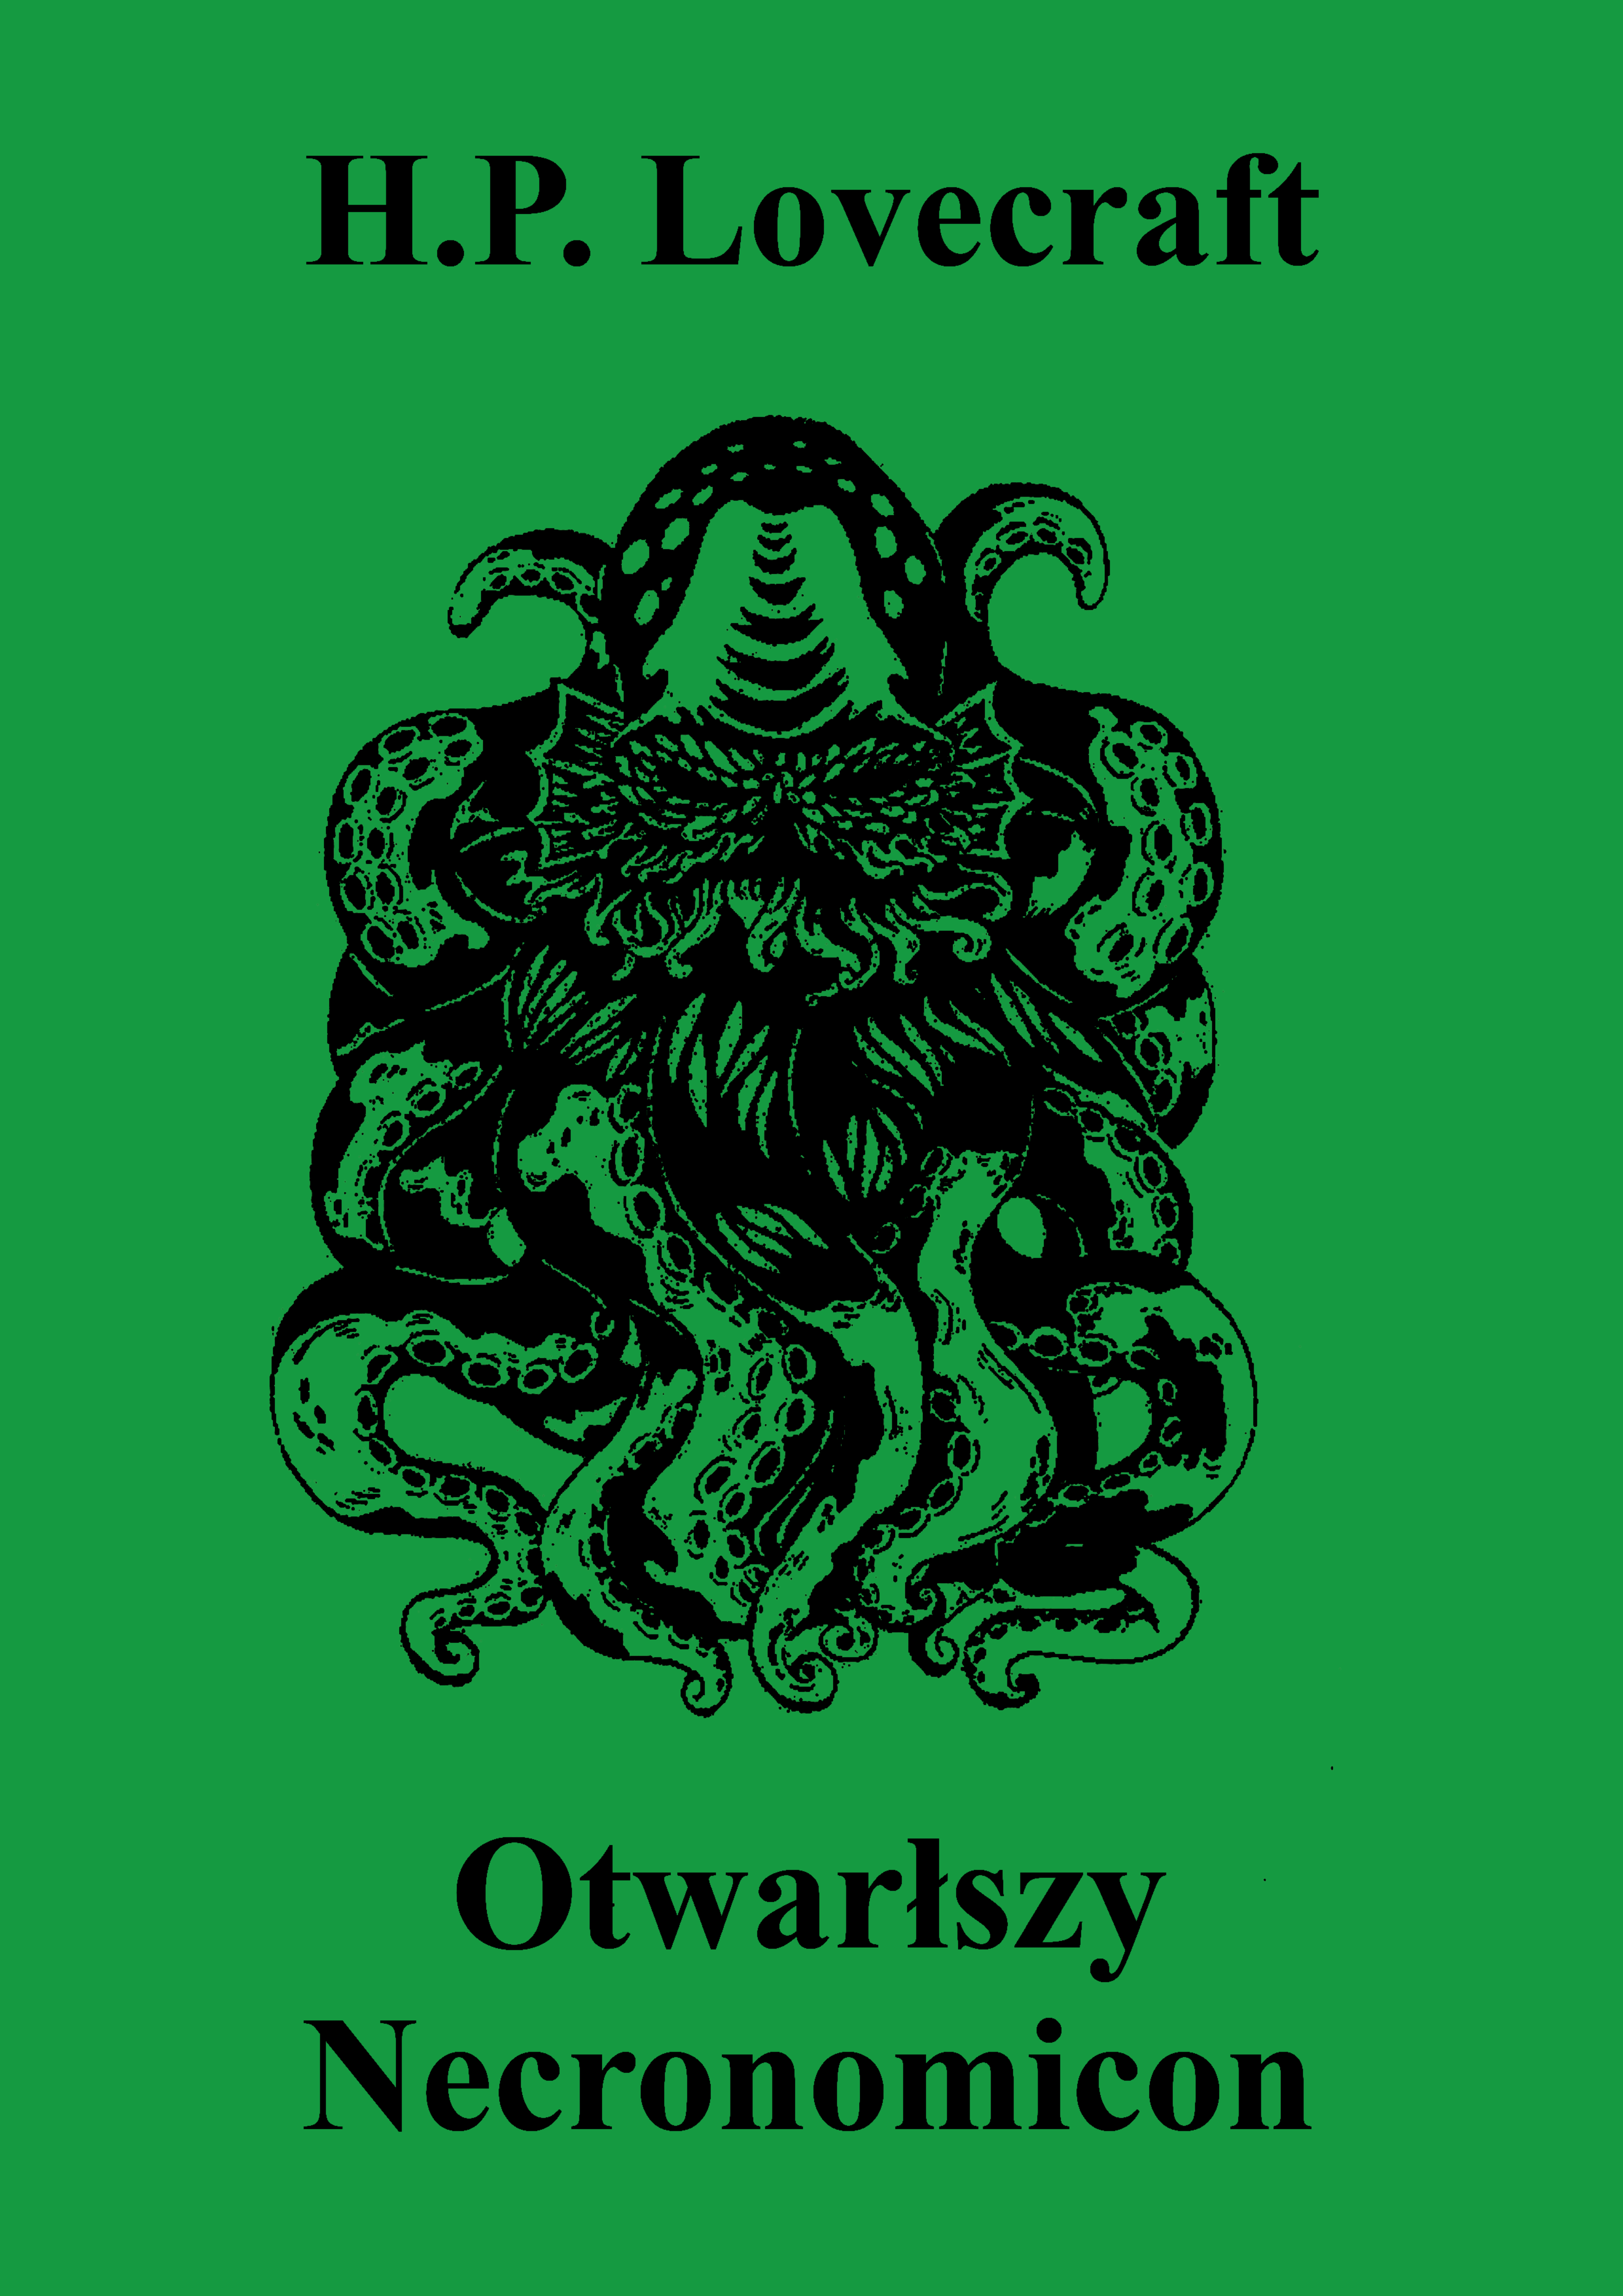
\includepdf[pages=1, noautoscale=true, width=\paperwidth]{Cthulhu-all-black.pdf}

\begin{titlepage}
	\centering
	{\Huge \bfseries \title _Otwarłszy Necronomicon \par}
	\vspace{1cm}
	{\large \itshape Zbiór tekstów H.P. Lovecrafta \par}
	{\large \itshape  w tłumaczeniu na licencji \textbf{CC-BY-SA 4.0} \par}
	\vspace{1cm}
	{\large \textbf{Teksty}: Copyright © H.P. Lovecraft \par}
	{\large \textbf{Tłumaczenie}: Copyright © \Year{\the\year} Szymon Brycki \par}
	\vspace{1cm}
	{\large \textbf{Obrazek na okładce}: \break Copyright © 2013 Marianna Rojas.  \break Licencja:  CC BY-NC-SA 2.0 \par}
	\vspace{1cm}
	{\large Stworzono w technologii \LaTeX \par}
	\vspace{1cm}
	{\large \today \par}
\end{titlepage}

\tableofcontents

% Teraz literówki, zacznij od rozdziału 4 !!!

\part{Powieść}

\chapter{Przypadek Charlesa Dextera Warda}
\index{Dzieła!Przypadek Charlesa Dextera Warda}
\index{Osoby!Charles Dexter Ward}
\index{Osoby!Dr. Willett}
\index{Osoby!Dr. Waite}
\index{Osoby! Dr. Lyman}
\index{Osoby!Joseph Curwen}
\index{Osoby!Jabez Bowen}
\index{Osoby!Dr. Checkley}
\index{Osoby!John Merritt}
\index{Osoby!Dutie Tillinghast}
\index{Osoby!Eliza Tillinghast}
\index{Osoby!Ezra Weeden}
\index{Osoby!Samuel Winson}
\index{Osoby!John Graves}
\index{Osoby!Cosmo Alexander}
\index{Osoby!Stephen Hopkins}
\index{Osoby!Joseph Brown}
\index{Osoby!Benjamin West}
\index{Osoby!Daniel Jenckes}
\index{Osoby!Eleazar Smith}
\index{Osoby!Manuel Arruda}
\index{Osoby!Harry Leshe}
\index{Osoby!Admiral Wallace}
\index{Osoby!Kolektor Robinson}
\index{Osoby!Kapitan James Mathewson}
\index{Osoby!Dr. Benjamin West}
\index{Osoby!Wielebny James Manning}
\index{Osoby!Stephen Hopkins}
\index{Osoby!John Carter}
\index{Osoby!John Brown}
\index{Osoby!Joseph Brown}
\index{Osoby!Nicholas Brown}
\index{Osoby!Moses Brown}
\index{Osoby!Dr. Jabez Bowen}
\index{Osoby!Kapitan Abraham Whipple}
\index{Osoby!Joseph Wanton}
\index{Osoby!Daniel Green}
\index{Osoby!Jedediah Orne}
\index{Osoby!Edward Hutchinson}
\index{Osoby!Luke Fenne}
\index{Osoby!Arthur Fenner}
\index{Osoby!Charles Slocum}
\index{Osoby!Simon Orne}
\index{Osoby!Wielebny Thomas Bernard}
\index{Osoby!Hepzibah Lawson}
\index{Osoby!Sędzia Hathorne}
\index{Osoby!Amity How}
\index{Osoby!Sędzia Gedney}
\index{Osoby!George Burroughs}
\index{Osoby!Sam Carew}
\index{Osoby!Mr. Parson}
\index{Osoby!Walter Dwight}
\index{Osoby!Naphthali Field}
\index{Osoby!Robert Hart}
\index{Osoby!Sierżant Riley}
\index{Osoby!Theodore Howland Ward}
\index{Osoby!Fred Lemdin}
\index{Osoby!Dr. Allen}
\index{Osoby!Gomes}
\index{Osoby!Dr. Peck}

\section{Rozdział Pierwszy: Wynik i Prolog}

\begin{center}
1
\end{center}

Z prywatnego szpitala dla chorych psychicznie, położonego w pobliżu Providence, Rhode Island, ostatnio zaginęła pewna szczególna osoba. Nosiła ona imię Charles Dexter Ward, i została umieszczona w zakładzie z wielkim żalem przez rozpaczającego ojca, któremu przyszło patrzeć, jak aberracja wzrasta ze zwykłego ekscentryzmu w mroczną manię zawierającą w sobie zarówno możliwość morderczych tendencji, jak i specyficznej zmiany w zawartości umysłu Charlesa. Psychiatrzy byli dosyć zaskoczeni tym przypadkiem, gdyż prezentował on dziwactwa zarówno psychologicznej, jak i fizjologicznej natury

Po pierwsze, pacjent wydawał się dziwnie starszy niż swoje 26 lat. Psychiczne rany, jeśli są prawdziwe, mogą postarzyć znacząco, lecz twarz tego młodego człowieka zawierała subtelne cechy, które normalnie uzyskują tylko ludzie wskutek starości. Po drugie, jego organiczne procesy wykazywały pewne dziwne właściwości, bez porównania z doświadczeniem medycznym doktorów. Oddychanie i praca serca wykazywały zaskakujący brak symetrii, głos jego został utracony, tak, że mógł on jedynie szeptać, trawienie trwało zaskakująco długo, w dodatku odbywało się w stopniu minimalnym, a reakcje neuronów na standardowe bodźce były nieporównywalne z wcześniejszą wiedzą medyczną, o organizmach zdrowych czy też chorych. Skóra Charlesa była sucha i o szarawym, nieświeżym odcieniu, a struktura komórkowa jego tkanek wydawała się być bardzo uszkodzona i ledwo się trzymająca razem. Nawet wielkie znamię w kształcie oliwki na jego prawym biodrze zaniknęło. W tym samym czasie, na jego klatce piersiowej uformował się wielki pieprzyk lub czarny punkt, którego tam wcześniej nie było. Ogólnie rzecz ujmując, wszyscy doktorzy zgadzali się ze sobą, że Ward posiadał metabolizm, który został uszkodzony w stopniu wykraczającym poza wcześniejsze precedensy.

Psychologicznie Charles Ward także był wyjątkowy. Jego szaleństwo nie miało sobie równych w zapiskach nawet najnowszych i najdokładniejszych rozpraw naukowych i encyklopedii medycznych, i towarzyszyła mu moc mentalna która mogłaby z niego uczynić geniusza lub przywódcę, gdyby nie wykrzywiono jej w dziwną i groteskową formę. Dr. Willett, który był lekarzem rodzinnym Wardów, potwierdza, że czyste zdolności psychiczne pacjenta, mierzalne poprzez jego reakcje na świat poza sferą jego szaleństwa, w zasadzie wzrosły od momentu pierwszego ataku. Ward, jest to prawdą, był zawsze uczonym i bibliofilem, ale nawet jego najgenialniejsze z wczesnych prac nie pokazywały jego jasności intelektu i przenikliwości, którymi się wykazywał podczas swoich rozmów z alienistami. Zaiste, było trudną rzeczą pozyskanie prawniczej zgody na przyjęcie go do szpitala, tak potężny i jasny zdawał się umysł tego młodego człowieka - tylko przy pomocy silnych dowodów i wielu anormalnym dziurom w jego zasobie informacji w kontraście do jego inteligencji, został on ostatecznie przyjęty do ośrodka. Aż do momentu jego zniknięcia był omni-czytelnikiem i tak dobrym rozmówcą, jak jego biedny głos tylko zezwolił. Uważni obserwatorzy, nie mogąc przewidzieć jego ucieczki, przewidzieli jednak, że nie minie dużo czasu, nim zostanie zwolniony ze szpitala.

\begin{center}
2
\end{center}

Tylko Dr. Willett, który odebrał poród Charlesa Warda i opiekował się wzrostem jego ciała i umysłu od tamtego czasu, wydawał się być przerażony na myśl o jego potencjalnej wolności. Miał on okropne doświadczenie i dokonał straszliwego odkrycia, którego nie ważył się wyjawić swym kolegom-sceptykom. Willett, zaiste, jest pomniejszą tajemnicą na swoich własnych zasadach w połączeniu z tym przypadkiem. Był ostatnim, który widział swego pacjenta przed jego ucieczką, i wyszedł z owej ostatniej konwersacji w stanie będącym mieszanką przerażenia i ulgi, co niektórzy wspominali, gdy ucieczka Warda stała się znana 3 godziny później. Ta ucieczka jest jedną z nierozwiązanych tajemnic szpitala Dr. Waite'a. Okno otwarte wysoko, na wysokości sześciu stóp raczej nie oferowało wyjaśnienia, lecz dalej, po tamtej rozmowie z Willettem młodzieniec niewątpliwie zniknął. Willett nie miał żadnego oficjalnego wyjaśnienia do zaoferowania, choć wydawał się być dziwnie zrelaksowany w stosunku do czasu sprzed ucieczki. Wielu, owszem, czuło, że chciałby powiedzieć coś więcej, lecz milczał z obawy przed niewiarą. Odnalazł on Warda w jego pokoju, lecz krótko po jego odejściu pielęgniarze pukali na nic. Kiedy otworzyli drzwi, pacjenta już tam nie było, a wszystko, co odkryli, to otwarte okno, przez które wiał chłodny, kwietniowy wietrzyk, rozsiewając wokół chmurę błękitno-szarawego pyłu, który prawie ich zadusił. Owszem, psy wyły jakiś czas wcześniej, ale to było wtedy, gdy Willett dalej rozmawiał z pacjentem, a nikt nie znalazł żadnego człowieka lub innej rzeczy, która wyjaśniałaby zniknięcie. Ojciec Warda został poinformowany natychmiastowo za pomocą telefonu, ale wydawało się, że jest on bardziej zasmucony niż zaskoczony. Do czasu, gdy Dr. Waite zadzwonił osobiście, Dr. Willet już z nim zdążył porozmawiać i obydwoje nie wiedzieli nic o ucieczce lub pomocy w niej. Tylko od pewnych bardzo sekretnych przyjaciół Willetta i starszego Warda pozyskano pewne wskazówki, a nawet one były zbyt fantastyczne, by brać je poważnie. Jedyny fakt który nam pozostaje to to, że na czas obecny nie ma żadnego śladu uciekającego szaleńca.

Charles Ward był antykwariuszem od swoich lat dziecięcych, niewątpliwie pozyskując swój gust ze starego miasta wokół niego i z reliktów przeszłości, które wypełniały każdy kąt starej willi jego rodziców przy Prospect Street na wzgórzu. Wraz z latami, jego oddanie antycznym przedmiotom tylko się zwiększyło, tak, że historia, genealogia i studiowanie kolonialnej architektury, mebli i rzemiosła wyrzuciły z jego umysłu wszelkie inne zajęcia. Te gusta są ważne do zapamiętania, rozważając jego szaleństwo, gdyż choć nie stanowią jego całkowitego centrum, odgrywają w nim znaczącą rolę. Luki w wiedzy, które alieniści dostrzegli były wszystkie powiązane z współczesnymi sprawami i były zakryte przez znaczącą wiedzę o sprawach dawno minionych, co wykazały przesłuchania: ktoś mógłby pomyśleć, że pacjent przeniósł się tutaj dosłownie z jednej ze starych epok poprzez jakaś osobliwą formę auto-hipnozy. Dziwną rzeczą było to, że Ward nie wydawał się już dłużej zainteresowany antykami, które znał tak dobrze. Miał, wynika, stracić wszelkie uznanie dla nich ze względu na dobrą znajomość, i jego ostatnie wysiłki było wszystkie poświęcone zdobyciu mistrzostwa w powszechnych faktach dnia codziennego, które kompletnie wyparowały z jego umysłu. To, że to kompletnie zaćmienie zdolności mentalnych nastąpiło, było czymś, co starał się on ukryć. Było to jednak oczywiste dla każdego, kto go obserwował, że jego cały program czytania i konwersacji był zdeterminowany przez życzenie pozyskania wiedzy o swoim własnym życiu i zwykłych praktycznych i kulturowych sprawach XX wieku, zgodnie z jego narodzinami w 1902 i edukacją w szkołach naszych czasów. Alieniści teraz się zastanawiają, jak z punktu widzenia jego uszkodzonej wiedzy, pacjent-uciekinier radzi sobie we współczesnym świecie; dominuje opinia, że ``zaszył się gdzieś'' do czasu, aż jego wiedza o świecie współczesnym powróci.

Początki szaleństwa Warda są kwestią dyskusyjną pośród alienistów. Dr. Lyman, eminentny autorytet z Bostonu, umieścił ją gdzieś w 1919 lub 1920, podczas ostatniego roku chłopaka w Moses Brown School, gdy nagle zwrócił się od studiów nad historią w stronę studiów okultystycznych, i odmówił wysłaniu dokumentów na uniwersytet na bazie indywidualnych badań o znacznie większym znaczeniu dla niego. To z pewnością jest powiązane z jego zmienionymi nawykami w tamtym czasie, zwłaszcza jego ciągłemu przeczesywaniu zapisków historii miejskiej i starych miejsc pochówku szukając pewnego konkretnego grobu z 1771 - grobu jego przodka imieniem Joseph Curwen, którego niektóre dokumenty znalazł ukryte w starym domu na Olnej Court, na wzgórzu Stempers, o którym jest wiadome, że Curwen go zamieszkiwał. 

Jest niewątpliwie oczywiste, że zima 1919-1920 przyniosła wielką zmianę w Wardzie, gdyż zaprzestał swoich badań antykwariusza i skupił się wyłącznie na desperackich badaniach nauk okultystycznych zarówno w domu jak i za granicą, przetykane tylko jego dziwnie stałym poszukiwaniem grobu swego przodka.

Jednakże, w tym momencie pojawia się sprzeciw Dr. Willetta, bazując swoją opinię na bliskim i ciągłym kontakcie z pacjentem, i na pewnych przerażających badaniach i odkryciach, których sam dokonał. Te badania i odkrycia odcisnęły na nim swoje piętno - jego głos się załamuje, gdy o nich opowiada, takoż jego dłoń drży, gdy próbuje o nich pisać. Willett przyznaje, że zmiana z 1919-1920 normalnie oznaczałaby początek postępującej dekadencji, która zakończyła się okropnie smutną i niespotykaną alienację z 1928, ale wierzy osobiście, że bardziej jasny rozdział powinien zostać poczyniony. Zgadza się on, że temperament młodzieńca zawsze był podatny na choroby psychiczne, i że był nadmiernie chętny w swoich odpowiedziach na zjawiska wokół niego, odmawia on przyznania, że te wczesna zmiana oznaczała przejście od poczytalności do szaleństwa, powołując się na słowa samego Warda, że odkrył coś, co najpewniej było wspaniałe i kluczowe dla historii myśli ludzkiej.

Prawdziwe szaleństwo, doktor jest pewien, nastąpiło wraz z późniejszą zmianą - po tym jak portret Curwena i jego antyczne dokumenty ujrzały światło dzienne, po tym, jak wykonano podróże do dziwnych, zagranicznych lokacji, i pewne straszliwe inwokacje zostały wyrecytowane w dziwnych i sekretnych okolicznościach, po tym, jak pewne \textit{odpowiedzi} na te inwokacje zostały jawnie wskazane, a pośpieszny list napisany w kondycji niewyjaśnionej agonii został napisany, po fali wampiryzmu i tajemniczej plotce o Pawtuxet, i po tym, jak z pamięci pacjenta usunięte zostały wszelkie wspomnienia współczesnych czasów  przy jednoczesnym osłabieniu jego głosu i jego fizyczności subtelnie zmienionej, co już wykazano wyżej.

Dopiero w tamtym czasie, Willett wskazuje z dokładnością, koszmarne cechy stały się stalą częścią Warda, i doktor jest przerażająco pewny, że istnieje dostatecznie dużo twardych dowodów, by potwierdzić twierdzenie młodzieńca o ważnym odkryciu. Po pierwsze, dwóch pracowników wysokiej inteligencji widziało antyczne dokumenty Josepha Curwena. Po drugie, sam chłopak kiedyś pokazał mu owe dokumenty i stronę z pamiętnika Curwena, i każdy z tych dokumentów posiadał autentyczny wygląd. Znana jest lokacja dziury, w której Ward znalazł owe zapiski, a sam Willett miał bardzo przekonujący ostatni rzut oka na nie w okolicznościach, którym ciężko jest dać wiarę i których być może nigdy nie udowodnimy. Dalej, są tajemnice i zbiegi okoliczności listów Orne'a i Hutchinsona, i problem pisma odręcznego Curwena i to, co detektywi odkryli o Dr. Allenie - te rzeczy i okropna wiadomość w średniowiecznych zapiskach odnalezionych w kieszeni Willetta po tym, jak odzyskał świadomość po swoim szokującym doświadczeniu.

Najważniejsze jednak są dwa okropne \textit{wyniki}, które doktor pozyskał z pewnej pary mistycznych formuł podczas swojego ostatecznego śledztwa - wyniki które udowodniły autentyczność dokumentów i ich potworne implikacje w tym samym czasie, jak i to, że te dokumenty zrodzone były z ludzkiej wiedzy.

\begin{center}
3
\end{center}

Należy spojrzeć na wcześniejsze życie Charlesa Warda jak na coś, co należy do przeszłości tak mocno, jak antyki, który sobie tam mocno ukochał. W jesieni 1918, i z pokazaniem wyraźnego zapału względem treningu wojskowego tamtego okresu, zaczął on swój pierwszy rok w Moses Brown School, która znajduje się nieopodal jego domu. Stary budynek główny, wzniesiony w 1819, zawsze był urokliwy dla oczu młodego antykwariusza - a rozległy park w którym mieści się Akademia oferował piękne widoki. Jego aktywności społeczne były mocno ograniczone, a swe godziny spędzał głównie w domu, na spacerach, w swoich klasach i w poszukiwaniu danych o antykach i genealogii w Urzędzie Miejskim, Domie Państwowym, bibliotece publicznej, Ateneum, Towarzystwie Historycznym, bibliotekach Uniwersytetu Brown, i nowo otwartej Bibliotece Shepley'a na Benefit Street. Można go sobie łatwo wyobrazić w tych dniach - wysokiego, chudego i o blond włosach, z uczonym okiem i lekko pochylonego, ubranego nieco niezgrabnie, i dającego wrażenie raczej niegroźnej niezdarności niż atrakcyjności. 

Jego spacery były zawsze przygodami powiązanymi z historią, podczas których był w stanie wyobrazić sobie miliony reliktów chwalebnej historii starego miasta i połączyć je z minionymi wiekami. Jego domem była okazała posiadłość w stylu georgiańskim, na szczycie stromego wzgórza, które wznosiło się na wschód przy rzece, a z jego tylnych okien mógł spojrzeć na ciasno upakowane wieżyce, stropy, dachy i drapacze chmur niższego miasta aż do purpurowych wzgórz poza miastem. To tutaj się urodził i z kochanego, klasycznego ganku fasady z podwójnie wypiekanych cegieł jego opiekunka prowadziła go w wózku, obok małej, białej farmy założonej 200 lat wcześniej i w kierunku budynków akademickich przy wystawnej ulicy, której stare, kwadratowe posiadłości z cegieł i mniejsze drewniane domy z wąskimi gankami opierającymi się na ciężkich kolumnach doryckich, były ustawione pośród przestronnych podwórek i ogrodów.

Był także prowadzony na wózku wzdłuż sennej uliczki Congdon Street, jeden poziom niżej na stromym wzgórzu, wraz z jej wschodnimi domami z wysokimi tarasami. Małe drewniane domki były najstarsze w tym miejscu, gdyż z tego właśnie wzgórza wzrastało rosnące miasteczko. To w tych podróżach przesiąkał on czymś w rodzaju koloru starej, kolonialnej wioski. Opiekunka miała w zwyczaju zatrzymać się i usiąść na ławkach Tarasu Prospekt, by porozmawiać z policjantami; jednym z pierwszym wspomnień tego dziecka był wielki, zachodni ocean dachów, kopuł i wież oraz odległe wzgórza które dostrzegł pewnego zimowego popołudnia z wielkiego wału z szynami, wszystkie fioletowe i mistyczne naprzeciwko rozgrzanego, apokaliptycznego zachodu słońca, malującego niebo czerwienią, złotem, purpurą i różnymi odcieniami zieleni. Szeroka, marmurowa kopuła Domu Stanowego wyróżniała się swoją masywną sylwetką, posąg będący jego ukoronowaniem otoczony fantastyczną aureolą poprzez szparę w jednej z stratusowych chmur, które lśniły na ognistych niebiosach. 

Gdy był starszy, rozpoczęły się jego słynne spacery; najpierw z jego niecierpliwie zaciągniętą opiekunką, a potem samotnie, w marzycielskiej medytacji. Głębiej i głębiej w ulice tego prawie pionowego wzgórza miał się zapuszczać, za każdym razem sięgając starszych poziomów tego antycznego miasta. Zatrzymywałby się niepewnie przy wejściu do Janckes Street z jej murami z tyłu i kolonialnymi szczytami sięgającymi aż do ciemnej Benefit Street, gdzie ukazywał mu się drewniany antyczny dom z parą drzwi w stylu jońskim, a obok niego był prehistoryczny dom z dachem mansardowym, gdzie zachowała się jeszcze resztka farmy, a także dom wielkiego sędziego Durfee z jego upadłymi pozostałościami stylu Georgiańskiego. To tutaj miały powstać slumsy, ale wielkie drzewa wiązów rzucały odżywczy cień na to miejsce, a chłopiec zwykł udawać się stąd na południe, wzdłuż długiej linii domów sprzed czasów Rewolucji Amerykańskiej, z wielkimi strychami i klasycznymi portalami. Po wschodniej stronie budynki te były osadzone wysoko ponad piwnicami, z podwójnymi schodami z kamiennymi stopniami i młody Charles mógł z wielką łatwością wyobrazić je sobie takie, jakie musiały być, gdy ulica ta była jeszcze młoda, gdy frontony były świeżo pomalowane, a nie widocznie zużyte, jak w dniu obecnym. 

Od strony zachodniej, wzgórze schodziło w dół prawie tak stromo jak wyżej, aż do starej Town Street, którą założyciele miasta umieścili przy krawędzi rzeki w 1636 r. To tutaj mieściły się niezliczone małe pasy z pochylonymi małymi domkami wielkiej antyczności; i, choć był wielce zafascynowany, minęło wiele czasu, nim odważył się spenetrować ich archaiczny wzrost z lęku przed wejściemf w sen lub wrota do nieznanych horrorów. Odkrył on, iż jest znacznie mniej straszliwe spacerowanie dalej wzdłuż Benefit Street aż do żelaznych wrót ukrytego kościółka Św. Johna i tyłu Domu Kolonialnego z 1761 r. i do zbutwiałego cielska karczmy Golden Ball, gdzie niegdyś zatrzymał się Waszyngton. Na Meeting Street  - zwanej Gaol Lane i King Street w innych czasach - szukałby na wschodzie i dostrzegłby łuk schodów, wspinających się na wzgórze, a w dół, w kierunku zachodnim, dostrzegłby Szkołę Kolonialną ze starych cegieł,  śmiejącą się z antycznego znaku z głową Szekspira, gdzie \textit{Providence Gazette} i \textit{Country-Journal} były drukowane przed Rewolucją. Następnie pojawiał się przecudowny Kościół Pierwszych Baptystów z 1775 r., luksusowy widok z jego niepowtarzalną wieżą Gibbsa i Georgianskimi dachami i kopułami, unoszącymi się wysoko. Tutaj i w kierunku południowym sąsiedztwo stało się lepsze, w ostateczności wykwiłwszy w cudowną grupę wczesnych posiadłości; lecz dalej małe antyczne paski prowadziły w kierunku zachodnim, wydawawszy się duchami z ich wielo-spiczastymi archaizmami, i ociekającymi od błyszczącego rozkładu, gdzie stare nadbrzeża wspominają dumnie czasy Indii Wschodnich wśród poliglotów, rozkładających się sterów, sklepów żeglarskich z zamglonymi witrynami i nazwami ulic z dawna, które przetrwały aż po dziś dzień, takimi jak Packet, Bullion, Gold, Silver, Coin, Doubloon, Sovereign, Guilder, Dollar, Dime, i Cent.

Czasami, po tym, jak urósł wyższy i bardziej żądny przygód, młody Ward ruszał głębiej w dół, ku burzy chwiejnych domów, złamanych poprzecznic, schodów, wygiętych balustrad, ciemnych twarzy i nienazwanych zapachów, ciągnących się od South Main do South Water, szukając doków, gdzie zatoka i statki parowe się spotykały, i wracał w stronę północną niższymi poziomami magazynów z 1816 o stromych dachach i szeroką drogą Wielkiego Mostu. To tutaj rynek z 1773 dalej stoi na jego antycznych łukach. Na tej szerokiej drodze zwykł się zatrzymywać, by wypić z czary piękna starego miasta gdy to wznosiło się w stronę wschodnią, pełne Georgiańskich szczytów i ukoronowane nową kopułą Christian Science tak, jak Londyn jest koronowany kopułą katedry św. Paula. Najbardziej lubił docierać do tego punktu późnym popołudniem, gdy światło słoneczne dotykało rynku i antycznych dachów domów na wzgórzu i ich dzwonnic, malując je złotem, i rzuca swą magię pośród wyśnionych nadbrzeży, gdzie niegdyś indianie z Providence zwykli zarzucać kotwice. Po dłuższym przyjrzeniu się temu widokowi, zakręciłoby mu się w głowie z poetycką miłością, i wtedy zacząłby drogę powrotną do domu, mijając po drodze stary, biały kościół i wąskie, strome uliczki, gdzie złote błyski odbijałyby się w oknach i naświetlach umieszczonych wysoko ponad podwójnymi schodami z balustradami z kutego żelaza. 

Innymi razy, i w późniejszych latach, szukał on wyrazistych kontrastów: spędzając połowę swojego spaceru w rozpadających się kolonialnych regionach na północny wschód od swego domu, gdzie wzgórze opada na najniższy poziom do Stempers Hill z jego gettem murzyńskim\footnote{Ogólnie rzecz ujmując nie lubię ``słowa na M'' i wierzę, że nie powinno się z niego korzystać w języku polskim. Tutaj użyłem go, niejako wbrew sobie, gdyż (A) Lovecraft użył w oryginale słowa ``Negro'' i (B) wiem doskonale, że za życia posiadał on uprzedzenia rasowe. Pragnę jednak zaznaczyć, że właściwy język we współczesnej polszczyźnie to ``osoba czarnoskóra'' a nie słowo na M. (przyp. tłum.)}, gromadzącym się wokół miejsca, gdzie dyliżansy do Bostonu zwykły rozpoczynać swą podróż przed czasami Rewolucji. Drugą połowę swoich spacerów spędzał on na południowych ziemiach wokół ulic George'a, Benevolent, Power i Williamsa, gdzie stare wzgórze jest gruntem dla pięknych włości i odgrodzonych murami ogrodów oraz zielonych ścieżek, z którymi wiąże się tyle drogich wspomnień. Te podróże, razem z pilnymi studiami, które im towarzyszyły, z pewnością przyczyniły się do wielkiej wiedzy historycznej zamieszkującej umysł Charlesa Warda. Ilustruje to także mentalną podstawę, niejaki grunt, na który padłu nasiona tej pamiętnej zimy 1919-1920, która to poruszyła wydarzenia, które miały tak dziwny i straszliwy finał.

Dr. Willett jest pewien, że do tej okropnej zimy, zainteresowania historyczne Charlesa Warda były wolne od zaburzonej psychiki. Cmentarze były wtedy dla niego bez szczególnego znaczenia, poza ich wartością historyczną, a cokolwiek w stylu przemocy lub dzikiego instynktu było poza jego psyche. Wtedy, sunąc powoli, acz nieubłaganie, pojawił się ostateczny wynik jednego z jego badań genealogicznych z poprzedniego roku; wtedy, gdy odkrył wśród swoich przodków po stronie matki pewnego długowiecznego człowieka imieniem Joseph Curwen, który przybył z Salem w marcu 1692, i o którym krążyły plotki i historie, które trudno powtarzać w dobrym towarzystwie.

Pra-pra-pradziadek Warda, Welcome Potter, w 1785 wziął ślub z pewną ``Ann Tillinghast, córką Pani Elizy oraz Kapitana Jamesa Tallinghasta'', o której rodowodzie rodzina nie posiadała żadnych szczegółowych informacji. Pod koniec 1918, podczas szukania woluminu o pierwotnych danych historycznych, młody genealog natrafił na wpis opisujący legalną zmianę nazwiska, które w 1772 pani Eliza Curwen, wdowa po Josephcie Curwenie, przyjęła razem ze swoją siedmioletnią córką Ann, której nazwiskiem panieńskim było Tillinghast, uzasadniając ową zmianę ``iż imię jej Męża stało się publiczną Obrazą dla Rozumu, bazując na wiedzy o jego Chorobie, która potwierdza pewne powszechne, antyczne Plotki, tak więc nie pragnę być znana jako jego lojalna Żona, dopóki owe plotki nie okażą się Bzdurne ponad wszelką wątpliwość''. Ten wpis ujrzał światło dzienne po przypadkowej separacji dwóch kartek, które ostrożnie sklejono razem i które były wyłączone z skądinąd poprawnej numeracji stron.

Było od razu oczywiste dla Charlesa Warda, że odkrył nieznany wcześniej sekret swojego pra-pra-pra-pradziadka. Odkrycie podnieciło go szczególnie, gdyż już słyszał ogólne raporty i widział rozsiane pogłoski o tej osobie, odnośnie której pozostało tak mało weryfikowalnych danych, pomijając te nieliczne, które ujrzały światło dzienne dopiero we współczesnych czasach, tak, że prawie zdawało się to być spiskiem, mającym na celu usunięcie go z ludzkiej pamięci. To, co jednak wydawało się płynąć z tych danych, miało tak prowokacyjną naturę, że nie dało się wyobrazić sobie, co powodowało, że owi kolonialni kronikarze byli tak pełni lęku i chętni, by ukryć i zapomnieć, lub by podejrzewać, że powody owego wykasowania były aż zanadto właściwe. 

Przed tym, Ward był wielce kontent, mogąc wyobrażać sobie starego Josepha Curwena jako coś zawieszonego w powietrzu - ale odkrywszy swoją własną relację z ową ``wymazaną'' figurą, zaczął szukać o nim danych tak systematycznie, jak to tylko możliwe. W tym ekscytującym zadaniu, ostatecznie odniósł on sukces poza swoimi największymi spekulacjami, gdyż stare listy, pamiętniki i nieopublikowane wspomnienia znalezione w zakurzonych strychach Providence i innych miast i miasteczek były obfite w wiele oświecających zapisków, odnośnie których ich autorzy nie uznali za stosowne, by je zniszczyć. Jedna ważna informacja pochodziła ze źródła tak odległego jak Nowy York, gdzie pewne zapiski kolonizatora z Rhode Island przechowywane były w Muzeum Frances' Tavern. Najważniejszą rzeczą jednak, i było to coś, co zdaniem Doktora WIlleta stanowiło ostateczne źródło klęski Warda, było coś, co znalazł w sierpniu 1919 za panelami starego domu w Olney Court. To było to, ponad wszelką wątpliwość, co otworzyło przed nim owe ciemne wizje, które kończyły się daleko poza dnem piekielnym. 

% TUTAJ SKOŃCZONE

\newpage

\section{Rozdział Drugi: Przodek i Horror}

\begin{center}
1
\end{center}

Joseph Curwen, co wyjawiły szeptane legendy odkryte przez Warda, był niezwykłym, enigmatycznym, w tajemniczy sposób okrutnym indywiduum. Uciekł z Salem do Providence - ostatecznego schronienia dla dziwnych, wolnych i niezgadzających się z powszechnie przyjętym konsensusem - na początku wielkiej paniki wiedźm. Bał się on prześladowań ze względu na samotniczy tryb życia i dziwne chemiczne czy też alchemiczne eksperymenty. Był on osobą o szarej skórze około trzydziestki, i szybko został obywatelem Providence, zakupiwszy później dom na północ od włości Gregory'ego Dextera na wysokości Olney Street. Jego dom był wybudowany na Stempers Hill na zachód od Town Street, w miejscu, które później zostało Olney Court. W 1761 zamienił ten dom na większy, przy tej samej ulicy, który dalej stoi w tamtym miejscu.

Warto zaznaczyć, że pierwszą dziwną rzeczą odnośnie Josepha Curwena było to, że zdawał się nie starzeć. Był zaangażowany w handel, zakupił miejsce na łódkę przy Mile-End Cove, pomógł odbudować Wielki Most w 1713 i Kościół Kongregacji na wzgórzu, ale zawsze posiadał wygląd mężczyzny, który nie miał więcej niż trzydzieści, może trzydzieści pięć lat. W miarę, jak dekady upływały jedna za drugą, ta cecha zaczęła przyciągać uwagę ludu. Curwen zawsze wyjaśniał, że pochodzi z długoletniego rodu, a za pośrednictwem prostego żywota uzyskał świetne zdrowie. Jak ową prostotę można pogodzić z niewyjaśnionymi zakupami sekretnego kupca i z dziwnymi światłami w oknach jego domu przez całą noc, nie było zbyt oczywiste dla mieszkańców miasta. Zamiast tego, postulowali one inne wyjaśnienie jego ciągłej młodości i długoletności. Istniał powszechny konsensus, że mieszanie przez Curwena tajemniczych chemikaliów było odpowiedzialne za jego stan. Plotki głosiły o dziwnych substancjach, które kupował z Londynu i Indii, transportowanych na jego statkach lub zakupionych w Newport, Bostonie lub Nowym Yorku, a gdy stary doktor Jabez Bowen przybył z Rehoboth i otworzył swoją aptekę po drugiej stronie Wielkiego Mostu, zwaną Pod Jednorożcem i Moździerzem, gorące szepty nie mogły zamilknąć o lekach, kwasach i metalach, które długowieczny odludek zakupił lub zamówił u niego. Działając w przekonaniu, iż Curwen posiadał cudowne i tajemnicze medyczne zdolności, wielu chorych ciągnęło do niego z prośbami o pomoc, lecz choć zdawał się on zachęcać ich wierzenia odnośnie samego siebie w luźny sposób, i zawsze dawał im mikstury w dziwnych kolorach w odpowiedzi na ich prośby, zauważono, że jego dary dla innych rzadko kiedy przynosiły im korzyści. Po upływie lat pięćdziesięciu, i bez większej zmiany niż 5 lat na jego licu, szepty ludzi stały się znacznie mroczniejsze. W efekcie, stał się jeszcze większym odludkiem.

Prywatne listy i pamiętnik z tego okresu ujawniają znacznie więcej powodów dla których Joseph Curwen był obiektem zdumienia, strachu, a w końcu potępiany niczym jakaś plaga. Posiadał pasję do cmentarzy, na których można go było dostrzec o każdej porze dnia i w każdych warunkach. Był z niej znany, choć nikt nie dostrzegł go nigdy czyniącego cokolwiek, co mogłoby być uznane za upiorne. Posiadał on farmę na Pawtuxet Road, na której spędzał czas w lecie, i na której często można było go dojrzeć, jeżdżącego konno o dziwnych godzinach dnia i nocy. Jego jedynymi znanymi sługami, farmerami i dozorcami była smutna para Indian z plemiona Narragansett - mąż głupi i pokryty bliznami, a żona z bardzo obrzydliwą twarzą, najpewniej ze względu na to, iż posiadała w sobie domieszkę czarnej krwi. W dobudówce do tego domu znajdowało się laboratorium, gdzie dokonywano większości chemicznych eksperymentów. Ciekawscy kurierzy, którzy dostarczali butelki, torby lub pudełka poprzez małe drzwi z tyłu rozsiewali plotki o fantastycznych flaszkach, tyglach, alembikach i piecach, które widzieli w niskim pomieszczeniu pełnym półek. Przepowiadali oni szeptem, że cichy ``chymik'' - przez co mieli na myśli \textit{alchemika} - wkrótce odkryje Kamień Filozoficzny. Najbliższe sąsiedzi tej farmy - Fennersowie, którzy znajdowali się o 1/4 mili dalej - mieli jeszcze dziwniejsze opowieści o pewnych dźwiękach, które, byli pewni, dochodziły z domu Curwena w środku nocy. Były to krzyki, mówili oni, i przeciągłe ryki. Nie lubili oni także wielkiej ilości zwierząt, które tłoczyły się na pastwiskach, gdyż tak wielka ich liczba nie była potrzebna by zapewnić staremu człowiekowi i paru sługom mięso, mleko i wełnę. Poszczególne zwierzęta w stadzie zdawały się zmieniać z tygodnia na tydzień, gdy nowe zwierzęta były zakupywane od rolników z Kingstown. Coś dziwnego było także odnośnie pewnego wielkiego, kamiennego budynku na uboczu, którego wysokie, wąskie szczeliny robiły za okna. 

Ludzie spotykani w pobliżu Wielkiego Mostu mieli dużo do powiedzenia o domu Curwena na Olney Court - nie o tym nowym wybudowanym w 1761, kiedy ten mężczyzna liczył sobie prawie wiek, lecz pierwszym - o niskim strychu pozbawionym okien i ścianami krytymi gontem, które spalił do cna po jego zdemolowaniu. Tutaj było mniej tajemnic, to prawda, ale godziny, o których widziano światła, sekretność dwóch obcokrajowców, którzy byli jedynymi sługami, ohydne szepty i dźwięki wydawane przez niesamowicie starego Francuza na usługach Curwena, wielkie ilości posiłków wchodzące przez drzwi, za którymi żyło tylko 4 ludzi, i ogólny \textit{wydźwięk} pewnych głosów często słyszanych w szeptanych rozmowach w dziwnych czasach - wszystko to razem połączone z tym, co było wiadome o farmie w Pawtuxet dało jej złowróżebną sławę.
 
W lepszych kręgach dom Curwena również był tematem rozmów. Nowoprzybyły,  naturalnie czynił znajomości w kościele i życiu społecznym miasta, znajomości lepszego sortu, których towarzystwo i konwersacje w oczywisty sposób sprawiały mu przyjemność. Jego urodzenie było wiadomie dobre, gdyż Curwenowie lub Carwenowie z Salem nie wymagali przedstawienia nikomu w Nowej Anglii. Było ewidentne, że Joseph Curwen podróżował dużo za młodu, żyjąc przez pewien czas w Anglii i pokonując co najmniej dwie podróże do Orientu. Jego mowa, gdy tylko miał taką potrzebę, była językiem wykształconego, kulturalnego Anglika. Ale z pewnego powodu Curwen nie dbał o swoją pozycję społeczną. Choć nigdy nie odmawiał otwarcie gościom, zawsze posiadał wokół siebie ścianę rezerwy, tak, że mało kto mógł pomyśleć o czymkolwiek do powiedzenia do niego, by nie zabrzmieć niczym szaleniec. 

Wydawało się, że sposób, w jaki Curwen się nosi, zawiera w sobie jakąś sekretną, sardoniczną arogancję, jak gdyby odkrył, że wszystkie istoty ludzkie są nużące po tym, jak bywał wśród dziwniejszych i bardziej potężnych istot. Kiedy Dr. Checkley, słynny w swym fachu, przybył do Bostonu w 1738, by zostać proboszczem w King's Church, nie omieszkał on wezwać tego, o którym słyszał tak wiele, ale odszedł po krótkiej chwili, której potrzebował, by wyczuć nutę zła w słowach jego gospodarza. Charles Ward powiedział swemu ojcu, że kiedy dyskutowali o Curwenie pewnego zimowego wieczora, że dałby wiele, by dowiedzieć się, co tajemniczy starszy mężczyzna powiedział młodemu kapłanowi, ale wszelcy autorzy pamiętników byli zgodni, że Dr. Checkley nie powtórzył niczego, co usłyszał. Ten dobry człowiek był naprawdę zaszokowany, i nigdy nie wspominał Josepha Curwena bez pewnej widocznej straty radości, z której był znany.

Istnieje jednak bardziej określony powód, dla którego inny człowiek wielkiego smaku i urodzenia unikał uczonego odludka. W 1746 pan John Merritt, starszy angielski dżentelmen o wykształceniu naukowym i literackim, przybył z Newport do miasta, które tak szybko się rozwijało i zaczął się budować w miejscu w Neck, które obecnie jest sercem najlepszej dzielnicy rezydenckiej. Żył on w wielkim stylu i komforcie, posiadając pierwszy dyliżans w mieście i zatrudniając dużo sług, i będać bardzo dumnym ze swojego teleskopu, mikroskopu i bardzo selektywnej biblioteki pełnej angielskich i łacińskich książek. Usłyszawszy, że Curwen jest posiadaczem najlepszej biblioteki w Providence, pan Merritt chętnie złożył mu wizytę, i został przyjęty grzeczniej niż większość innych gości w jego domu. Jego zachwyt półkami gospodarza wypełnionymi klasyką w angielskim, łacinie i grece z dodatkiem tekstów filozoficznych, matematycznych i naukowych, w których wliczał się Paracelsus, Agricola, Van Helmont, Salvius, Glauber, Boyle, Boerhaave, Becher i Stahl, sprawił, że Curwen zaproponował wizytę do swojej farmy i laboratorium, do których nigdy wcześniej nie zaprosił nikogo. Obydwoje ruszyli natychmiast w dyliżansie pana Merritta.

Pan Merritt zawsze twierdził, że nie dostrzegł niczego w oczywisty sposób bluźnierczego na farmie, ale utrzymywał, że tytuły książek w specjalnej bibliotece taumaturgicznej, alchemicznej i teologicznej, którą Curwen trzymał w przednim pokoju, były same w sobie dostateczne, by wywołać w nim uczucie głębokiego dyskomfortu. Być może jednak, to wyraz twarzy właściciela księgozbioru przyczynił się bardzo mocno do tego uprzedzenia. Niecna kolekcja, poza zbiorem standardowych dzieł, które nie zaalarmowały pana Merritta, posiadała w sobie niemal wszystkie dzieła kabalistyczne, demonologiczne i magiczne znane człowiekowi, i była prawdziwa skarbnicą wiedzy odnośnie wiedzy w wątpliwej domenie alchemii i astrologii. Hermes Trismogistus w edycji Mesnarda, \textit{Turba Philosopharum}, \textit{Liber Investigationis} Gabera i \textit{Klucz do Mądrości} Artephousa - wszystkie tutaj były, razem z kabalistycznym \textit{Zoharem}, zestawem \textit{Albertus Magnus} Petera Jamma, \textit{Ars Magna et Ultima} Raymonda Lully'ego w edycji Zetznera, \textit{Thesaurus Chemicus} Rogera Bacona, \textit{Clavis Alchimiae} Fludda, \textit{De Lapide Philosophico Trithemusa}. Średniowieczni Żydzi i Arabowie byli obecni w księgozbiorze aż zanadto, i pan Merritt był wstrząśnięty, gdy chwyciwszy z półki wolumin podejrzenie nazwany \textit{Qanooon-e-Islam}, odkrył, iż był to w istocie zakazany \textit{Necronomicon} szalonego Araba Abdula Alhazreda, o którym słyszał takie potworne rzeczy szeptane parę lat wcześniej po kontakcie z nienazwanymi rytuałami w dziwnej, małej wiosce Kingsport w zatoce Massachusetts.

Lecz co najdziwniejsze, szlachetny dżentelmen poczuł się najbardziej zniesmaczony przez malutki detalik. Na wielkim stole z z mahoniu leżała odkładką w dół znoszona kopia Borellusa, nosząca wiele tajemniczych, odręcznych zapisków stworzonych ręką Curwena. Książka była otwarta mniej-więcej w połowie, i jeden z paragrafów był podkreślony tak wyraźnymi liniami, że gość nie mógł się powstrzymać i zaczął go czytać. Niezależnie od tego, czy była to natura podkreślonego akapitu, czy gorączkowa natura linii tworzących podkreślenie - pan Merritt sam nie wiedział - ale coś w tej kombinacji wpłynęło na niego w sposób znaczący i złowieszczy. Mógł przywołać ten akapit z pamięci do końca swoich dni, zapisawszy go w swoim pamiętniku i raz spróbowawszy wyrecytować go swojemu bliskiemu przyjacielowi, Dr. Checkley'owi, choć przestał, zauważywszy, jak bardzo proboszcz czuł się poruszony owym cytatem .Stanowił on, iż:

\begin{displayquote}

Esencjalne Sole Zwierzęce mogą być tak przygotowane i przechowane, by inteligentny Człowiek posiadał całą Arkę Noego w swoim Studium, i wskrzesił Kształt Zwierzęcia z jego Popiołów dla swojej własnej Przyjemności, i podobną Metodą, z esencjalnych Soli ludzkiego Pyłu, Filozof może, bez zbrodni Nekromancji, wezwać Kształt dowolnego martwego Przodka z Pyłu w który jego Ciało się obróciło.

\end{displayquote}

To jednak doki w południowej części Town Street były miejscem, gdzie krążyły najgorsze pogłoski o Josephie Curwenie. Marynarze są bardzo przesądni i doświadczeni żeglarze, którzy przywozili nieskończone ilości rumu, niewolników i słupy melasy, szelmowscy korsarze i wielkie brygi Brownsów, Crawforsów i Tilliinghastów, wszyscy czynili znaki ochronne, kiedy widzieli chudego, podejrzenie młodo wyglądającego człowieka o żółtych włosach, lekko pochylonego, gdy wchodził do magazynu na Doubloon Street lub rozmawiającego z kapitanami na długim nabrzeżu, na którym statki Curwena płynęły bez ustanku. Księgowi i kapitanowie pracujący dla Curwena nienawidzili i bali się go, a wszyscy jego marynarze byli wzięci z Martinique, St. Eustatius, Havany lub Port Rolay. W pewien sposób, to częstotliwość, z jaką ci marynarze byli zmieniani, była powodem, który prowokował najbardziej materialną część lęku, który towarzyszył staremu człowiekowi. Jego załoga mogłaby się rozejść po mieście lub wybrzeżu, niektórzy z jej członków musieliby zrobić to czy tamto, a gdy ponownie by się spotkali, z całą pewnością brakowałoby im mężczyzny lub dwóch. Wiele owych rzeczy, które musieliby zrobić, dotyczyłoby farmy na Pawtuxet Road, i tak mało marynarzy kiedykolwiek wróciło z tego miejsca. Ten fakt tkwił wyraźnie w pamięci żeglarzy. W pewnym momencie przyczyniło się to do znacznego utrudnienia zamorskich biznesów Curwena. Ostatecznie paru z nich zostawiłoby statki za swoimi plecami, po usłyszeniu plotki o nabrzeżach Providence, i ich zastępcy musieli pochodzić aż z Indii Zachodnich, co stało się dużym problemem dla kupca.

W 1760 Joseph Curwen był ostatecznym wyrzutkiem, podejrzewanym o nieokreślone zbrodnie i demoniczne przymierza, które wydawały się tym straszniejsze, że nie mogły być nazwane, zrozumiane, lub choćby udowodnione, jakoby istniały. Ostatni gwóźdź do trumny był problem z zaginionymi żołnierzami z 1758, gdyż w marcu i kwietniu tego roku  dwa królewskie regimenty stacjonowały w Providence, na trasie do Nowej Francji. Żołnierze ci znikali bez śladu ponad spodziewaną liczbę dezercji. Od razu podniosły się plotki o częstotliwości, z jaką Curwen był widziany, rozmawiając z obcymi w czerwonych płaszczach, a gdy paru z nich zostało uznanych za zaginionych, ludzie wrócili myślami do dziwnych przypadłości jego własnych marynarzy Co by się stało, gdyby regimenty nie ruszyły dalej, tego nikt nie jest w stanie powiedzieć. 

W międzyczasie, materialne sprawy kupca prosperowały. Posiadał w praktyce monopol na handel saletry potasowej, czarnym pieprzem i cynamonem, i z łatwością przewodził handlowi innymi dobrami, z pierwszeństwem być może Brownsów w jego imporcie indygo, wyrobów mosiężnych, bawełnianych i wełnianych, soli, żelaza, papieru i wszelkich dóbr korony brytyjskiej. Tacy sklepikarze jak James Green z Słonia w Cheapside, Russelowie z Złotego Orła po drugiej stronie Mostu, lub Clark i Nightingale z Ryby i Patelni w pobliżu New Coffee-House, polegali prawie całkowicie na nim, by zaopatrywać się w towary, i jego biznesy z lokalnymi warzelniami alkoholu, mleczarzami i hodowcami konii z plemienia Narragansett i twórcami świec z Newport, uczyniły z niego jednego z głównych eksporterów w całej Kolonii.

Choć był on niewątpliwie ofiarą ostracyzmu społecznego, potrafił być miły, w pewien sposób. Kiedy Dom Kolonialny spalił się do fundamentów, pomógł wtedy skrzywdzonym pokaźną sumą, która pozwoliła wybudować nowy budynek, z cegieł - ciągle stojący niczym przewodniczący paradzie na starej głównej ulicy. Działo się to w 1761 r. W tym samym roku, pomógł on odbudować Wielki Most po załamaniu chmury w październiku. Odbudował on wielką część księgozbioru biblioteki publicznej, którą pochłonął pożar Domu Kolonialnego. Wsparł także loterię, która dała błotnistemu Market Parade i Town Street chodniki z wielkich, obłych kamieni, aby można było się komfortowo poruszać na piechotę. Mniej-więcej w tym samym czasie, wybudował on prosty lecz piękny nowy dom, którego drzwi były tak wielką zdobyczą sztuki płaskorzeźby. Kiedy wierni z Whitefield odseparowali się od kościoła na wzgórzu Dr. Cottona w 1743 i założyli kościół w Deacon Snow po drugiej stronie Mostu, Curwen wyruszył z nimi, choć jego wiara religijna szybko nie okazała się zbyt żarliwa. Teraz, jednak, stał się wierzący po raz kolejny, jakby próbując odrzucić cień, który wymusił na nim izolację i który wkrótce miał zacząć niszczyć jego biznesy, gdyby czegoś z tym nie zrobił. 

Widok tego dziwnego, bladego mężczyzny, wyglądającego na będącego ledwie w wieku średnim, lecz z pewnością nie młodszym niż stulecie, który zapragnął wreszcie wyłonić się z chmury lęku i zohydzenia zbyt uogólnionych, by je dookreślić lub zanalizować, był zarówno żałosny, dramatyczny i ohydny. Jednakże, taka jest moc bogactwa i powierzchownych gestów, że zaiste, objawiło się niskie obniżenie w widocznej awersji pokazywanej mu przez gmin - zwłaszcza po tym, jak nagłe zaginięcia jego żeglarzy przeminęły jak z bicza strzelił. Musiał on także zacząć stosować ekstremalną ostrożność i sekretność odnośnie swoich wypraw na cmentarz, gdyż nigdy później już go nie przyłapano na krążeniu po nim. Podobnie, pogłoski o dziwnych dźwiękach i światłach w jego posiadłości w Pawtuxet także stały się mniej częste. Jego zapotrzebowanie na żywność i bydło pozostało niewytłumaczalnie wysokie. Dopiero w czasach Charlesa Warda, którzy prześwietlił jego rachunki i dokumenty w Shepley Library, uderzyło go, jako jedynego, że można porównać wielką liczbę Czarnych z Guinei, których importował aż do 1766 z bardzo małą ich liczbą, która była oddawana handlarzom niewolników w Wielkim Moście lub do plantacji w Narragansett Country. Z pewnością, bystrość i geniusz tej okropnej, nieludzkiej osoby były oczywiste, gdy już uświadomiło się ich ogrom.

Ale oczywiście, efekt tych wszystkich zabiegów naprawczych był raczej znikomy. Curwen dalej był unikany przez swoich pobratymców - zaiste, wszyscy zazdrościli mu długowieczności. Mógł on dostrzec, że w efekcie jego bogactwa z pewnością musiały na tym ucierpieć. Jego skomplikowane studia i eksperymenty, niezależnie od tego, czego dotyczyły, najwyraźniej wymagały wielu pieniędzy, aby móc je kontynuować. Gdyby plotki wreszcie wpłynęły na jego zarobki - gdyby pozbawić go przychodu z handlu, które pozyskał, nie pomogłoby mu zaczęcia od nowa w innym miejscu. Osąd sytuacyjny wymagał, że powinien naprawić swoje relacje z mieszkańcami miasta Providence, tak, aby jego obecność już nie była powodem szeptanych konwersacji, wybitnie oczywistych wymówek nagłych obowiązków i ogólnej atmosfery powstrzymania się i niezręczności. Jego pracownicy, zredukowani obecnie do bezczynnych i zmęczonych cieni, których nikt inny by nie zatrudnił, przysparzali mu wielu problemów. Co zaś do jego kapitanów i marynarzy, trzymał ich przy sobie dzięki przebiegłości i przewagom, które pozyskał nad nimi - takiej jak weksle, hipotekę lub posiadanie informacji potrzebnych, by ich szantażować. W wielu przypadkach, twórcy pamiętników odnotowywali z niejakim zdziwieniem, że Curwen posiadał prawie magiczną moc śledzenia rodzinnych sekretów, które następnie wykorzystywał w wątpliwych celach. Podczas ostatnich 5 lat jego życia, wydawało się, że tylko bezpośrednie rozmowy z dawno zmarłymi ludźmi mogły mu zapewnić ogrom informacji, które trzymał na końcu swego języka. 

Mniej-więcej w tym samym czasie, zręczny uczony wykonał ostatnią próbę, by wrócić do łask lokalnej społeczności. Do tego momentu kompletny pustelnik, teraz zapragnął zawrzeć korzystny związek małżeński, biorąc za żonę kobietę, której wysoka pozycja społeczna uczyniłaby wszelkie próby ostracyzmu względem niego niemożliwymi. Mozliwe, że miał również inne, ważniejsze powody, by zawrzeć takie małżeństwo - powody na tyle oddalone od normalnej logiki, że tylko zapiski znalezione półtora wieku później, po jego śmierci, sprawiły, że ktokolwiek mógł ich podejrzewać. O tym jednak nic pewnego nie może zostać w pełni poznane. Naturalnie, był on świadom horrorów i upokorzeń związanych z uwodzeniem, które spotkałyby jego osobę, tak więc szukał odpowiedniej kandydatki, na której rodzicach mógłby wywrzeć stosowną presję. Takie kandydatki, odkrył, nie były tak proste do odnalezienia, gdyż miał on swoje bardzo konkretne wymagania odnośnie ich piękna, osiągnięć i poważania w społeczeństwie. Jego wymagania zawęziły możliwy wybór do domu jednego z jego najlepszych i najstarszych kapitanów, wdowca wysokiego urodzenia i nieposzlakowanej opinii imieniem Dutie Tillinghast, którego jedyna córka Eliza posiadała wszelkie możliwe przewagi, z wyjatkiem zostania dziedziczką rodu. Kapitan Tillinghast był kompletnie zdominowany przez Curwena - i zgodził się, po koszmarnym wypytywaniu w swoim kopulastym domu na wzgórzu Power's Lane, pobłogosławić ten bluźnierczy mezalians. 

Eliza Tillinghast miała w tamtym czasie 18 lat i została wychowana tak łagodnie, jak pozwoliły na to warunki w skromnym domu jej ojca. Chodziła do szkoły Stephena Jacksona po drugiej stronie Court House Parade i była uczona przez swoją matkę, zanim ta umarła na ospę w 1757 r., odnośnie wszelkich sztuk domowego żywota. Przykład jej kunsztu, stworzony w 1753 r. można dalej znaleźć w pomieszczeniach Towarzystwa Historycznego Rhode Island. Po śmierci jej matki zajmowała się ona domem, wspierana tylko przez jedną starą, czarnoskórą kobietę. Jej kłótnie z jej ojcem odnośnie propozycji malżeńskiej Curwena musiały być zaiste burzliwe, lecz nie mamy o nich żadnych świadectw. Jest jednak pewne, że jej narzeczeństwo względem młodego Ezry Weedena, drugiego oficera na statku Enterprise pod dowództwem Crawforda, zostało odwołane, a jej związek z Josephem Curwenem wszedł w życie siódmego marca 1763 r. Miało to miejsce w kościele Baptystów, w obecności najznamienitszych gości, jakich tylko miasto mogło zgromadzić, ceremonii zaś przewodził młody Samuel Winson. The Gazette wspomniała o zawarciu małżeństwa w paru zdaniach, a w większości kopii, które przetrwały, ta krótka wzmianka była wycięta lub wyrwana. Ward odnalazł jedną jedyną kompletną kopię po wielu godzinach poszukiwań w archiwach prywatnego kolekcjonera, rozbawiony bezsensownym miejskim językiem wzmianki:

\begin{displayquote}

W poniedziałek wieczorem, Pan Joseph Curwen, z naszego Miasta, Kupiec, ożenił się z Panną Elizą Tillinghast, Córką Kapitana Dutie'go Tillinghasta, młodą panienką prawdziwej Wartości, dodanej do Piękna jej Osoby, co uświętni Stan Małżeński i pomnoży jego Szczęście.

\end{displayquote}

Kolekcja listów Durfee-Arnolda, odkryta przez Charlesa Warda tuż przed jego pierwszym załamaniem nerwowym w prywatnej kolekcji Melville'a F. Petersa z George Street, i obejmująca tamten i poniekąd wcześniejszy okres, rzuca wyraźne światło na publiczne oburzenie na ten źle dobrany związek małżeński. Społeczne wpływy Tillinghastów, jednakże, były niezaprzeczalne, i po raz kolejny Joseph Curwen odkrył, że jego dom stał się odwiedzany przez osoby, których w innych okolicznościach w ogóle nie przepuściłby przez swój próg.  Jego akceptacja tego faktu nie była wszak kompletna, a jego żona cierpiała społecznie ze względu na wymuszone przedsięwzięcie, ale poprzez kolejne wydarzenia udało im się uniknąć ostracyzmu społecznego. W jego traktowaniu swojej żony, dziwny pan młody zaskoczył zarówno nią, jak i szerszą społeczność, poprzez ukazywanie ekstremalnego taktu i wdzięczności. Nowy dom w Olney Court był teraz zupełnie wolny od dziwnych manifestacji, a choć Curwen w dużej mierze porzucił farmę w Pawtuxet, której jego żona nigdy nie odwiedzała, wyglądał teraz bardziej jak normalny człowiek niż w jakimkolwiek innym momencie swojego wcześniejszego, długiego życia. Tylko jedna osoba pozostała z nim w otwartej wrogości - wspomniany młody oficer, z którym zaręczyny Eliza Tillinghast zerwała. Ezra Weeden całkiem otwarcie poprzysiągł zemstę Curwenowi i, choć zazwyczaj był łagodnego usposobienia i manier, nabierał teraz nienawistnego poczucia celu, które nie wróżyło dobrze mężowi-uzurpatorowi.

Siódmego dnia maja 1765 roku, urodziło się jedyne dziecko Curwena, Ann, ochrzczona przez Wielebnego Johna Gravesa z King's Church, do którego zarówno mąż, jak i żona zapisali się wkrótce po ślubie, jako kompromis pomiędzy ich dwoma wcześniejszymi wspólnotami religijnymi - Congregationalnej i Baptystów. Zapisy tych narodzin, jak i ślubu 2 lata wcześniej, zostały usunięte z większości kopii kościelnych i dokumentów miejskich, gdzie powinny były się pojawić. Charles Ward zdołał odnaleźć obydwa z wielką trudnością po jego odkryciu, iż wdowa zmieniła swe imię, co poinformowało go o jego własnej relacji z nim, i zagroziło gorączkowymi poszukiwaniami, które miały swoją kulminację w jego szaleństwie. Zapiski o porodzie, zaiste, zostały odkryte bardzo ciekawe poprzez korespondencję ze spadkobiercami lojalisty Dr. Gravesa, który zabrał ze sobą duplikaty zapisków kiedy opuścił miasto na początku Rewolucji. Ward spróbował zasięgnąć informacji u tego źródła, będąc w pełni świadomym, że jego pra-pra-babka, Ann Tillinghast Potter, należała do wspólnoty Episkopalnej.

Wkrótce po narodzinach swojej córki, wydarzeniu, które świętował z przytupem odmiennym od swojej zwykłej oziębłości, Curwen postanowił zapozować do portretu. Został on namalowany przez bardzo utalentowanego Szkota imieniem Cosmo Alexander, które w tamtym czasie zamieszkiwał Newport, słynny od tamtego czasu jako nauczyciel Gilberta Stuarta. Podobiezna, mówili ludzie, została wykonana na drewnianym panelu ściennym w bibliotece domu w Olney Court, lecz żaden z dwóch pamiętników, które o nim wspominały, nie informował o jego ostatecznym losie. W tamtym okresie nasz kapryśny uczony wykazywał oznaki nienaturalnej abstrakcji, i spędzał tak wiele czasu, jak to tylko możliwe na swojej farmie przy Pawtuxet Road. Zdawał się on, było mówione, być w stanie ukrywanego podniecenia lub oczekiwania; tak jakby spodziewał się jakiejś fenomenalnej rzeczy lub był w przededniu ważnego odkrycia. Zdawało się, że chemia lub alchemia odgrywa w tym wielką rolę, gdyż zabierał on ze swojego domu do farmy wielką liczbę woluminów w tych właśnie tematach.

Jego zainteresowanie sprawami miasta się nie zmniejszyło, i nie tracił żadnej okazji, by pomóc liderom pokroju Stephena Hopkinsa, Josepha Browna lub Benjamina Westa w ich wysiłkach, by ubogacić kulturowo miasto, które w tamtych czasach było znacznie poniżej Newport jeśli chodzi o patronat nad sztukami wyzwolonymi. Pomógł on Danielowi Jenckesowi otworzyć jego księgarnię w 1763, i był później jej najlepszym klientem - pomógł także Gazette w kłopotach, ukazującej się każdej środy w Pod Głową Szekspira. W polityce, żarliwie wspierał gubernatora Hopkinsa przeciwko Wardom, którzy głównie siedzieli w Newport, a jego naprawdę elokwentna przemowa w Hacher's Hall w 1765 przeciwko separacji Północnego Prowidence jako osobnego miasta, stanowiła główny z powodów, dla których spadły w  mieście uprzedzenia względem niego. Ale Ezra Weeden, który obserwował go z bliska i uważnie, prychał cynicznie pod nosem na jego wszelkie aktywności życia publicznego, i jawnie przysięgał, że było to nic więcej jak ledwie maska, skrywająca pod sobą najczarniejszą z istot Tartaru. Mściwy młodzianin rozpoczął systematyczne studium mężczyzny i jego działań, kiedykolwiek był w porcie, spędzając godziny w nocy razem z łowcami wielorybów, w oczekiwaniu na światła z posiadłości Curwena, i podążając za małą łódeczką, która czasami usuwała się po cichu z zatoki. Trzymał on też rękę na pulsie jeśli chodzi o farmę Pawtuxet, co kiedyś zakończyło się poważnym pogryzieniem przez psy, które stara para Indian puściła na niego. 

\begin{center}
2
\end{center}

Do jesieni roku 1770 Weeden zadecydował, że należy działać nagle i zwrócił na siebie uwagę ciekawskich mieszczan, gdyż w powietrzu unosił się aromat niespodziewanych, nagłych wydarzeń, zrzucony niczym stary płaszcz, dając miejsce trudno ukrywanemu wyniesieniu perfekcyjnego triumfu. Curwen wydawał się mieć problem z powstrzymaniem siebie samego przed publicznymi przemówieniami o tym, co on odkrył lub czego się dowiedział, lecz najwyraźniej, potrzeba utrzymanie owej rzeczy w tajemnicy była większa niż jego pragnienie, ażeby się pochwalić odkryciem, gdyż nigdy nie zaoferował on żadnego wyjaśnienia. To po tych wydarzeniach, które najpewniej miały miejsce we wczesnym lipcu, złowróżebny badacz zaczął zaskakiwać ludzi posiadaniem informacji, które tylko ich dawno zmarli przodkowie mogli posiadać.

Lecz sekretne aktywności Curwena w żadnym wypadku nie zostały wstrzymane wraz z tą zmianą. Wprost przeciwnie, raczej się one zwiększyły, tak, że więcej i więcej jego biznesów pozostawało w rękach kapitanów statków, którzy byli teraz z nim związani zarówno więzami strachu, równie potężnymi jak i wizją bankructwa. Porzucił on w zupełności handel niewolnikami, twierdząc, że przychody z niego ciągle się zmniejszały. Każdą wolną chwilę spędzał on na farmie w Pawtuxet, choć tu i ówdzie pojawiały się pogłoski o jego obecności w miejscach, które, choć nie były technicznie w pobliżu cmentarzy, to były z nimi powiązane na tyle mocno, iż ludzie zaczęli się dziwić, czy aby stary kupiec nie powrócił do swoich starych nawyków - a może po prostu nigdy z nimi nie zerwał? Ezra Weeden, choć szpiegował go w krótkich okresach, ze względu na swoje morskie podróże, śledził go z mściwą wytrzymałością, której większość mieszczan i rolników nie posiadało, i badał sprawy Curwena z dokładnością, z którą nigdy wcześniej nie były one badane. 

Wiele dziwacznych manewrów statków kupca można było wytłumaczyć niespokojnością owych czasów, w których każdy kolonista starał się oprzeć założeniom Sugar Act, co skutkowało problemami w transporcie. Smuglowanie i unikanie zadomowiły się dobrze w Narragansett Bay, a nocne cumowania nielegalnych ładunków były bardzo upowszechnione. Ale Weeden, noc po nocy, podążał za światłami statków i małych łodzi, które wracały od magazynów Curwena przy docu Town Street, wkrótce też zdał sobie sprawę z tego, że nie tylko statki Jego Królewskiej Mości były tym, czego chciał uniknąć Curwen. Przed zmianą z 1766, te łodzie najczęściej zbierały skutych Murzynów, którzy byli transportowani poprzez zatokę i lądowali w mało znanym miejscu tuż na północ od Pawtuxet, skąd przemieszczali się do farmy Curwena, gdzie ich zamykano w ogromnym kamiennym budynku, który posiadał wąskie szczeliny zamiast okien. Potem jednak, cały program zmieniono. Zaprzestano importu niewolników, i przez pewien czas Curwen osierocił swe transporty o północy. Wtedy, około wiosny 1767, nowa polityka weszła w życie. Po raz kolejny jego statki opuściły ciche, ciemne doki, i tym razem opuściły zatokę, unosząc się na morzu w pewnym dystansie, może nawet na wysokości Nanquit Point, gdzie miały się spotkać z dziwnymi statki wielkiego rozmiaru i różnorodnego wyglądu, ażeby odebrać od nich ładunki. Następnie, marynarze Curwena mieli zdeponować te ładunki w zwykłym miejscu na wybrzeżu, i przetransportować je lądem do jego farmy, zamykając je w tym samym tajemniczym budynku z kamienia, w którym wcześniej przebywali Murzyni. Ładunki te prawie w całości składały się z pudeł i pudełek, z których duża część była wielka i ciężka, oraz zaskakująco przypominająca wyglądem trumny.

Weeden zawsze obserwował farmę z nieustanną pilnością, odwiedzając ją każdej nocy przez dłuższy czas, i rzadko kiedy pozwalając, by minął tydzień bez jego obserwacji, z wyjątkiem dni, gdy grunt był pokryty śniegiem ukazującym ślady piechura. Nawet wtedy jednak, często podchodził tak blisko, jak to tylko możliwe, korzystając z dobrze uczęszczanych dróg lub lodu na pobliskiej rzece, by patrzeć na ślady, które inni mogli zostawić. Odkrywszy, że jego własne śledztwo staje na drodze jego morskich obowiązków, zatrudnił on lokalnego bywalca karczmy, imieniem Eleazar Smith, aby kontynuował badania, gdy zleceniodawca przebywał daleko. Obydwoje mogliby puścić w głos pewne niezwykle dzikie pogłoski. Nie zrobili tego tylko i wyłącznie dlatego, że znali efekt, jaki rozgłos mógłby wywołać na ich ofierze i uczynić dalszy postęp śledztwa niemożliwym. Zamiast tego, chcieli się dowiedzieć czegoś konkretnego zanim by zaczęli działać. To, czego się dowiedzieli, musiało zaiste być przerażające, i Charles Ward mówił wiele razy swoim rodzicom o swoim żalu z powodu tego, że Weeden później spalił swoje notatniki. Wszystko, co można powiedzieć o ich odkryciach to to, co Eleazar Smith zanotował w swoim niezbyt rozsądnym dzienniku,  i co inni pisarze pamiętników i listów skromnie powtarzali, gdy już pewne słowa się rozniosły - i zgodnie z którymi farma była tylko zewnętrzną skorupą jakiejś szeroko rozpowszechnionej i obrzydliwej okropności, której zasięg i głębia była zbyt ważna i nieuchwytna, by pozyskać coś więcej niż iluzję zrozumienia. 

Udało się potwierdzić, że Weeden i Smith byli przekonani, że obszerna sieć tuneli i katakumb znajdowała się pod farmą, i była zamieszkana przez rozlicznych ludzi, poza starą parą Indian. Dom ten był starym reliktem środka XVII wieku z pokaźnym kominem i oknami z kratami w kształcie diamentów, a laboratorium wysuwało się ku północy, w miejscu, gdzie grunt prawie stykał się z dachem. Ten budynek zdawał się przypominać każdy inny, lecz zważywszy na różne głosy słyszana czasami w jego wnętrzu, z pewnością musiał do niego prowadzić sekretny, podziemny korytarz. Te głosy, przed 1766, były ledwie szeptami i majakami Murzynów, niekiedy przechodzącymi w paniczne wrzaski, przemieszane z intrygującymi inwokacjami i modłami. Po tej dacie, jednakże, przyjęły one formę bardzo dziwnego i okropnego dźwięku, mieszaniny tępego przyzwolenia i wybuchów szaleńczej furii, wraz z konwersacjami i sapaniami oraz okrzykami protestu. Wydawało się, że mówione były różne języki, wszystkie znane Curwenowi, których akcenty były często nierozróżnialne - odpowiedzi, potwierdzenia czy groźby?

Czasami zdawało się, że parę osób musi być w domu: Curwen, pewni pojmani i strażnicy owych pojmanych. Były to głosy, których ani Weeden, ani Smith nigdy wcześniej nie słyszeli pomimo ich rozległej wiedzy o obcych portach, i wielu zdawało się należeć do tej czy innej narodowości. Natura tych konwersacji zawsze zdawała się być rodzajem katechizmu, tak jakby Curwen odzyskiwał pewne informacje od przerażonych lub buntowniczych więźniów. 

Weeden posiadał wiele dosłownych raportów z podsłuchanych fragmentów wypowiedzi w swoich notatkach, mówionych po angielsku, francusku i hiszpańsku, które to języki znał i które były często używane - lecz z owych notatek nic się nie ostało. Jednakże, powiedział on, że poza paroma grobowymi dialogami dotyczącymi przeszłych wydarzeń w życiach rodzin z Providence, większość pytań i odpowiedzi, które mógł zrozumieć, było historycznych lub naukowych; czasami dotyczyły one bardzo odległych miejsc lub czasów. Przy jednej okazji, przykładowo, na zmianę wściekła i pokorna osoba były przesłuchiwana po francusku o masakrę Czarnego Księcia w Limoges w 1370, zupełnie jakby był w tej historii jakiś sekret, który powinna ona znać. Curwen zapytał więźnia - jeśli był on więźniem - o to, czy rozkaz zabicia był wydany ze względu na Znak Kozy znaleziony na ołtarzu w antycznej rzymskiej krypcie pod katedrą, lub czy Czarny Człowiek z kowenu Haute w Wiedniu wymówił Trzy Słowa. Nie mogąc uzyskać odpowiedzi, inkwizytor najwyraźniej posunął się do ekstremalnych środków, gdyż rozległ się przerażający wrzask, a następnie cisza, szeptanie i odgłosy uderzania.

Żadne z tych rozmów nie zostały nigdy wizualnie potwierdzone, gdyż zasłony w oknach były zawsze ciężko zasunięte. Jednak raz, podczas rozmowy w nieznanym języku, można było dostrzec zza zasłon cień w oknie, który przeraził Weedera znacząco. Przypominał mu on o marionetkach w teatrzyku dla lalek, który zaobserwował na jesień 1764 w Hacher's Hall, kiedy mężczyzna z Germantown w Pensylwanii zaprezentował sprytny mechaniczny spektakl reklamowany jako ``Widok na Słynne Miasto Jerozolimę,, w którym można dostrzec Jerozolimę, Świątynię Salomona, Królewski Tron, ważne Wieże i Wzgórza, jak i Cierpienie Naszego Zbawcy z Ogrodu w Gethsemane na Krzyżu na wzgórzu Golgota, prawdziwie artystyczny Pomnik. Warte zobaczenia przez Ciekawych Świata''. To przy tamtej sposobności podsłuchiwacz, który zakradł się blisko okna z przodu, gdzie miała miejsce rozmowa, został przerażony przez parę starych Indian, którzy puścili na niego swoje psy. Po tym wydarzeniu nie było już słychać bluźnierczych konwersacji w domu, a Weeden i Smith uznali, że Curwen musiał przenieść swoje operacje w podziemne regiony domostwa.

To, że takie regiony musiały po prawdzie istnieć, wydawało się oczywiste z wielu powodów. Odległe krzyki i jęki dochodziły tu i ówdzie ze, zdawałoby się, solidniej ziemi pod stopami, w miejscach odległych od jakichkolwiek budowli. Jednocześnie, ukryta pośród krzaków przy rzece z tyłu, gdzie wysoki grunt przechodził w dolinę Pawtuxet, znajdowała się drewniana brama, którą, w momencie odkrycia, uznano za będącą wejściem do jaskiń pod wzgórzem. Kiedy i jak owe katakumby zostały wzniesione, Weeden nie mógł powiedzieć, ale często wskazywał na to, jak łatwo owe miejsce mogłoby zostać dosięgnięte przez bandy niewidzialnych pracowników rzecznych. Joseph Curwen pokierował swoich morskich przyjaciół do różnych celów, zaiste! Podczas ciężkich deszczy roku 1769 dwójka obserwatorów trzymała oko na rzece by sprawdzić, czy jakiekolwiek podziemne sekrety ujrzą światło dzienne, i nagrodzono ich, gdy zobaczyli zarówno kości zwierzęce, jak i ludzkie na brzegu rzeki. Oczywiście, mogło to mieć wiele wyjaśnień, w pobliżu farmy i starego cmentarza Indiańskiego, ale Weeden i Smith doszli do swoich własnych konkluzji. 

Był styczeń 1770, gdy Weeden i Smith dalej próżno debatowali co, jeśli cokolwiek, myśleć lub zrobić odnośnie całej tej zastanawiającej sprawy, kiedy nastąpił wypadek z Fortalezą. Rozczarowani z powodu utraty swojego zysku ze statku Liberty w Newport poprzedniego lata, flota celna dowodzona przez Admirała Wallaca zaadoptowała politykę uważniejszej kontroli odnośnie dziwnych statków, i z tej okazji uzbrojony szkuner Jego Wysokości, nazwany Cygnet, pod dowództwem kapitana Harry'ego Leshe'a, pochwycił, po krótkim pościgu pewnego poranka, statek Fortaleza z Barcelony w Hiszpanii, którym dowodził kapitan Manuel Arruda, a który przewoził ładunek z Cairu w Egipcie do Providence. Kiedy przeszukano go w celu znalezienia kontrabandy, statek ten okazał się przewozić wyłącznie egipskie mumie, do odbioru przez ``Marynarza A. B. C.'', który miał się pojawić i opróżnić ładownię w Nanquit Point, a którego tożsamość Kapitan Arruda czuł się związany honorem, by utrzymać w tajemnicy. Sąd Vice-Admiralski w Newport, nie wiedząc co zrobić w obliczu legalności całego transportu z jednej strony, a niepraworządną tajemniczością odbiorcy z drugiej, dokonał kompromisu i z rekomendacji Kolektora Robinsona pozwolił statkowi na wypłynięcie, ale zabronił mu dokować w wodach Rhode Island. Później niosły się plotki, że widziano go w przystani bostońskiej, choć nigdy oficjalnie nie wstąpił do portu bostońskiego.  

Ten niezwykły incydent był na językach w Providence i niewielu wątpiło w istnienie jakiegoś połączenia między transportem mumii a złowieszczym Josephem Curwenem. Jego egzotyczne badania i intrygujące eksperymenty chemiczne były wiedzą powszechną, a jego uwielbienie cmentarzy wywoływało w tym kontekście podejrzenia - nie wymagało wielkiej wyobraźni połączenie tego z wydarzeniem, które nie miało innego wyjaśnienia w mieście. Jakby świadom tego oczywistego faktu, Curwen dbał o to, by wypowiedzieć się niby mimochodem przy paru okazjach o chemicznej wartości balsamów znajdowanych w mumiach, być może sądząc, że mógłby on uczynić całe wydarzenie bardziej naturalnym i nieszkodliwym, jednakże zostało to przez wielu odebrane jako przyznanie się do winy. Weeden i Smith, oczywiście, byli przekonani o ważkości tego wydarzenia, i snuli najdziksze teorie o Curwenie i jego straszliwych sprawkach.

Następnej wiosny, jak w roku wcześniejszym, nastąpiły ciężkie ulewy, a obserwatorzy ostrożnie patrzyli na poziom wody w rzece za farmą Curwena. Wielkie sekcje ziemi zostały zmyte, i odkryto przy okazji pewną liczbę kości, ale nie istniało żadne wejrzenie w podziemnie komnaty lub kryjówki. Jednakże, jak głosiła plotka,  coś się wydarzyło w wiosce Pawtuxet, milę dalej, gdzie rzeka wpływa i spada ze skalistego tarasu, łącząc się ze spokojną, zamkniętą w lądzie pokrywą. W tym miejscu, pełnym starych domków wiejskich wspinających się na wzgórze ze staro-szkolnym mostkiem, i z rybackimi kutrami czekającymi w sennych dokach, pewien raport głosił, że pewne rzeczy płynęły w dół rzeki i ukazywały się oczom ludzi przez minutkę, gdy spadały wraz z wodospadem. Oczywiście, Pawtuxet to długa rzeka która płynie przez wiele osiedli ludzkich, gdzie istnieją także cmentarze, i oczywiście, wiosenne ulewy były bardzo intensywne, ale rybacy przy moście nie lubili dzikiego spojrzenia, którym jedno z ciał wpatrywało się w nich, gdy ginęło w wodzie poniżej, lub krzyku drugiego, choć jego stan zdawał się nie pozwalać na żadne krzyki. Ta plotka sprawiła, że Smith - Weeden był wtedy na morzu - ruszył szybko do brzegu rzeki za farmą, gdzie owszem, znalazł dowody zaawansowanego zapadnięcia się. Jednakże, nie było śladu dostępu do brzegu rzeki, gdyż miniaturowe lawiny zostawiły za sobą solidną ścianę mieszanki ziemi z krzakami z góry. Smith zdecydował się na eksperymentalne wykopki, ale zniechęcił go brak sukcesu - a może był to lęk przed możliwym sukcesem? Ciekawie jest zastanowić się, co wytrwały w swych dążeniach Weeden zrobiłby na jego miejscu, gdyby nie znajdował się na statku.

\begin{center}
3
\end{center}

W momencie, gdy jesień 1770 się rozpoczęła, Weeden zadecydował, że nadszedł czas, by poinformować innych o swoich odkryciach, gdyż zgromadził sporą liczbę faktów, a także posiadał drugiego świadka, gdyby pojawiły się oskarżenia, że wszystko wymyślił, kierowany zwykłą zazdrością. Jako pierwszą osobę, do której poszedł, wybrał Kapitana Jamesa Mathewsona, ze statku Enterprise, który z jednej strony znał go dostatecznie dobrze, by nie wątpić w jego słowa, a z drugiej był dostatecznie wpływowy w mieście, by zostać wysłuchanym z szacunkiem. Spotkanie odbyło się w górnym pokoju tawerny Sabina w pobliżu doków, z obecnym Smithem by potwierdzić każdą z opowieści - i można było dostrzec, że Kapitan Matthewson był pod wielkim wrażeniem. Jak prawie każda inna osoba w mieście, posiadał własne przemyślenia w temacie Josepha Curwena; tak więc potrzebował tylko tego potwierdzenia i większego zasobu informacji, by przekonać go absolutnie. Na końcu konferencji, był bardzo poważny, i poprosił resztę mężczyzn o zachowanie milczenia. Miał on, wyjaśnił, przekazać te informacje osobno około 10 najbardziej uczonym i ważnym osobom w Providence, zaznać ich porady i poznać ich poglądy, a następnie posłuchać ich zdania. Sekretność była tutaj kluczowa, gdyż nie były to problemy, z którymi lokalne siły porządkowe lub sądy mogłyby sobie poradzić. Także podekscytowany tłum powinien być trzymany w ignorancji, albowiem inaczej mogło dojść do drugich wydarzeń z Salem, co miało miejsce mniej niz wiek temu, a co sprowadziło Curwena do Providence.

Odpowiednio osoby, wyjaśnił, byłyby następujące: Dr. Benjamin West, którego traktat o późnym tranzycie Wenus udowodnił, że jest on uczonym i krytycznym myślicielem; Wielebny James Manning, Prezydent Kolledżu który właśnie się przeprowadził z Warren i chwilowo zamieszkiwał przy nowym budynku szkoły na King Street, czekając, aż zakończy się budowa na wzgórzu powyżej Presbyterian Lane; ex-Gubernator Stephen Hopkins, który był członkiem Towarzystwa Filozoficznego w Newport i był mężczyzną bardzo szerokich horyzontów; John Carter, wydawcą lokalnej Gazety; wszyscy 4 z braci Brown, John, Joseph, Nicholas i Moses, którzy stanowili uznanych lokalnych możnowładców, dodatkowo, Joseph był naukowcem-amatorem; stary Dr. Jabez Bowen, którego erudycja była sporych rozmiarów, i który posiadał wiedzę z pierwszej ręki o starych zakupach Curwena; i Kapitan Abraham Whipple, żeglarz fenomenalnej odwagi i energii, który mógłby przewodzić czynnościom, jeśli zajdzie potrzeba. Ci mężczyźni, jeśli by zapragnęli, mogliby zostać wezwani razem dla kolektywnych decyzji, i na nich spoczywałaby odpowiedzialność zadecydowania, czy poinformować lub nie Gubernatora Kolonii, Josepha Wantona z Newport, przed podjęciem akcji. 

Misja Kapitana Mathewsona odniosła sukces poza jego najdzikszymi oczekiwaniami, gdyż choć jeden albo dwóch z uczonych mężów pozostało sceptycznymi odnoście opowieści Weedena, nie było ani jednego, który nie uznał za stosowne podjęcie jakiegoś rodzaju sekretnej i skoordynowanej akcji. Curwen, co było jasne, stanowił zagrożenia dla dobra miasta i Kolonii, i powinno się go wyeliminować za wszelką cenę. Późno w grudniu 1770, grupa eminentnych mieszczan spotkała się w domu Stephena Hopkinsa i dabatowała o środkach, które należało podjąć. Notatki Weedena, które ten wręczył Kapitanowi Mathewsonowi, były ostrożnie i uważnie czytane, a sam Weeden i Smith zostali wezwani, ażeby odpowiedzieć na dodatkowe pytania. Coś podobnego do strachu zaczęło kiełkować w sercach zebranych nim spotkanie się skończyło, lecz także i poważna determinacja, najlepiej wyrażona przez Kapitana Whipple'a i jego twardą osobowość. Nie zamierzali oni poinformować Gubernatora, gdyż coś innego niż akcja natury prawnej jawiła im się jako rozwiązanie problemu. Z ukrytymi mocami niejasnej potęgi do swojej dyspozycji, Curwen nie był mężczyzną, któremu można było po prostu nakazać opuszczenie miasta. Co więcej, nawet, gydby kreatura opuściła miasto, byłoby to po prostu przesunięcie problemu w inne regiony geograficzne. Żyli oni w bezprawnych czasach, a ludzie, którzy przemycali przez lata ładunki poza percepcją Jego Królewskiej Mości, raczej nie robiliby sobie problemów z prawa. Curwen musiał zostać zaskoczony na swojej farmie w Pawtuxet przez dużą grupę doświadczonych korsarzy, i dostać ostatnią szansę, ażeby się obronił od oskarżeń. Gdyby okazał się szaleńcem, zabawiającym się w wykrzykiwane, wymyślone konwersacje różnymi głosami, należało znaleźć mu miejsce w odpowiednim przybytku. Jeśli cos mroczniejszego miało miejsce, a podziemne horrory miałyby okazać się prawdziwe, on i wszyscy u jego boku powinni umrzeć. Gdyby można było to zrobić cicho, należałoby tak uczynić, tak, by nawet wdowa i jej ojciec nie znali wszystkich szczegółów. 

Kiedy debatowano o tych poważnych krokach, koniecznych do podjęcia, nastąpił w mieście incydent tak straszliwy i niewyjaśnialny, że przez pewien czas nic innego nie było wspominane w obszarze wielu mili. W środku bezksieżycowej, styczniowej nocy z ciężkimi opadami śniegu, nad rzeką i wzgórzami rozległa się seria krzyków, która sprawiły, że śpiący pojawili się przy swoich oknach, a ludzie w okolicach Waybosset Point dostrzegli wielką białą rzecz, poruszającą się gorączkowo w źle oczyszczonej przestrzeni z przodu Turk's Head. W tle rozległo się szczekanie psów, lecz szybko się zakończyło, gdy dźwięki obudzonego miasta stały się głośniejsze. Grupy mężczyzn z muszkietami i latarniami ruszyły zobaczyć, co się wydarzyło, lecz ich poszukiwania niczego nie przyniosły. Następnego poranka, jednakże, wielkie, umięśnione i nagie ciało zostało znalezione na lodzie w południowej części Wielkiego Mostu, gdzie Długi Dok rozciągał się obok destylarni Abbotta, a tożsamość zmarłego stała się tematem niekończących się spekulacji i szeptów.Co ciekawe, to starsi mieszkańcy, a nie młodsi, szeptali między sobą, gdyż tylko pośród starszyzny ta zesztywniała twarz z oczami otwartymi w przerażeniu odwoływaa się do ich pamięci. Tak więc starsi, drżąc na ciele, wymieniali zaskoczone szepty zdziwienia i przerażenia, gdyż w tych okropnych rysach znaleźli zadziwiające podobieństwo, ba, wręcz identyczność z pewną osobą - osobą, która umarła całe 50 lat wcześniej.

Ezra Weeden był obecny podczas tego znaleziska, i pamiętając ujadanie psów poprzedniej nocy, ruszył wzdłuż Weybosset Street i w kierunku mostu Muddy Dock, skąd dochodził dźwięk. Miał ciekawe przeświadczenie, i nie był zaskoczony, kiedy dotarłszy na skraj dzielnicy mieszkaniowej, gdzie ulica zmieniała się w Pawtuxet Road, natrafił na intrygujące ślady w śniegu. Nagi gigant był śledzony przez psy i wielu mężczyzn w butach, a ślady powracających psów i ich panów mogły być łatwo wyśledzone. Poddali się oni dopiero, gdy dotarli zbyt blisko miasta. Weeden uśmiechnął się ponuro, i wyśledził ślady z powrotem do ich źródła - była to farma w Pawtuxet Josepha Curwena, zupełnie, jak się tego spodziewał. Oddałby on wiele, by podwórze nie było tak konfundująco zadeptane. Zważywszy na wszystko, nie chciał być zbyt zainteresowany w świetle dnia. Dr. Bowen, do którego Weeden zaraz się udał ze swoim raportem, dokonał autopsji dziwnego ciała, i odkrył pewne dziwności, które go kompletnie skołowały. Układ trawienny wielkiego człowieka zdawał się nigdy nie być w użyciu, a cała skóra była szorstka i luźno zwisała z ciała, czego nie dało się wyjaśnić w żaden sposób. Zaintrygowany tym, co starzy ludzi szeptali o podobieństwie ciała do dawno martwego kowala imieniem Daniel Green, którego prawnuk Aaron Hoppin służył na statku Curwena, Weeden zadawał pobieżne pytania, aż nie dowiedział się, gdzie Green został pochowany. Tej nocy grupa 10 mężczyzn odwiedziła North Burying Ground po drugiej stronie Herrenden's Lane i otworzyli ten grób. Znaleźli go pustym, dokładnie tak, jak się spodziewali.

W międzyczasie, poczyniono przygotowania i przechwycono korespondencją Josepha Curwena. Tuż przed inducentem z nagim ciałem, odnaleziono list od pewnego człowieka imieniem Jedediah Orne z Salem, który zmusił cooperujących obywateli do głębokiej zadumy. Część tego listu, skopiowana i przechowana w prywatnych archiwach rodziny, gdzie został znaleziony przez Charlesa Warda, brzmiał następująco: 

\begin{displayquote}

``Cieszy mnie, że kontynuujesz Swoje zainteresowanie Starymi Sprawami, lecz nie myśl, że inaczej było z Panem Hutchinsonem w wiosce Salem. Z pewnością, nie było tam Nic tylko najgorsze Okropności w tym, jak H. zebrał to, czego tylko część zebraliśmy my. To, co zrobiłeś nie Zadziałało, albo ponieważ Jakaś Rzecz zawiodła, albo ponieważ Twe Słowa nie były Dobrze Wymówione lub skopiowane. Sam nie Wiem. Nie posiadam Chemicznej wiedzy, by podążać za Borelliusem, i sam jestem skonfundowany przez Tę Księgę Nekronomiconu, którą polecasz. Ale proszę, Zauważ, że zwróciliśmy Ci Uwagę, żebyś Uważał kogo wzywasz, pamiętaj, co Pan Mather napisał w swych Uwagach ———, i zważ na to, jak ta Okropna rzecz jest raportowana. Mówię Ci ponownie, nie wzywaj Niczego, czego nie możesz odesłać, przez co mam na Myśli, Każdego, Kto może z Powrotem powstać przeciwko Tobie, gdy Twoje Potężne Urządzenie nie mogą być użyte. Pytaj o Pomniejszych, gdyż Wielcy nie będą chcieli Odpowiedzieć, i mogą mieć władzę większą od Twojej. Byłem przerażony, gdy przeczytałem, że wiesz co Ben Zaristnatmik zostawił w swym Hebanowym Podle, gdyż wiedziałem, kto musiał Ci to powiedzieć. I ponownie proszę, byś pisał do mnie per ``Jadediah'' a nie ``Simon''. W tej społeczności mężczyzna nie może żyć zbyt długo, a Ty znasz mój Plan, zgodnie z którym wróciłem jako mój Syn. Nie mogę się doczekać, aż mi Powiesz co ten Czarny Mężczyzna powiedział Ci o Sylvanusie Cocodiciusie w Twojej krypcie, pod Rzymskim murem, i będę zobligowanym, jeśli mi Pożyczysz tego MS. o którym tyle mówiłeś.''

\end{displayquote}

Inny list, niepodpisany, wysłany z Filadelfii, wywołał podobne zamieszania, zwłaszcza następujący fragment:

\begin{displayquote}

``Będę słuchał tego, co masz do Powiedzenia, ale tylko przez Twoich Posłańców, ale nie zawsze jestem pewien, kiedy się ich spodziewać. W Kwestii o której już mówiliśmy, proszę o tylko jedną rzecz więcej, lecz chcę do Ciebie podejść odpowiednio. Mówisz mi, że żadna Część nie może być zgubiona jeśli najlepszy Efekt ma się wydarzyć, ale nie możesz wiedzieć, jak ciężko być pewnym. Wydaje się to być wielkim Ryzykiem i Ciężarem, wziąć całe Pudło, a w Mieście (np: St. Peter's, St. Paul's, St. Mary, lub Christ Church) ciężko to zrobić w ogóle. Lecz znam wszystkie imperfekcje, które podniosłeś w ostatnim październiku, i jak wiele żywych Osobników musiałeś wykorzystać, by wejść w odpowiedni Stan w 1766, więc będę Cię słuchał we wszelkich Kwestiach. Nie mogę się doczekać Twojego Statku, i pytam oń co dzień w Mr. Biddle's Wharf''

\end{displayquote}

Trzeci podejrzany list był napisany w nieznanym języku, a nawet nieznanym alfabecie. W pamiętniku Smitha znalezionym przez Charlesa Warde, jedna często powtarzana kombinacja znaków została niezdarnie skopiowana; naukowcy w Brown University określili ten alfabet jako amharski lub abisyński, ale nawet oni nie rozpoznają tego słowa. Żadna z tych wiadomości nie została nigdy dostarczona do Curwena, lecz zaginięcie Jedediaha Orne'a z Salem została zanotowano jako nieco późniejsze wydarzenie, co pokazuje, że mężczyźni z Providence podjęli pewne ciche kroki. Towarzystwo Historyczne Pensylwanii także posiada pewien ciekawy list otrzymany przez Dr. Shippena odnośnie obecności niebezpiecznej postaci w Filadelfii.
Lecz ważniejsze kroki dopiero miały zostać podjęte, przez zgromadzenie zaprzysiężonych i przetestowanych marynarzy i korsarzy z magazynu w Bostonie w środku nocy - to był główny skutek odkryć Weedena. Powoli, lecz stanowczo, plan kampanii powstawał w sekrecie, plan kampanii która miała zostawić brak jakiegokolwiek śladu po tajemnicach Josepha Curwena. 

Curwen, pomimo wszystkich obostrzeń, najwyraźniej czuł, że coś się szykuje, gdyż wyglądał teraz na wielce zmartwionego. Jego powóz był widziany o wszelkich godzinach w mieście i na Pawtuxet Road, i trochę po trochu utracił swoją aurę wymuszonej dobrotliwości, którą starał się zwalczyć uprzedzenia mieszczan. Najbliżsi sąsiedzi jego farmy, Fannersowie, pewnej nocy zauważyli wielkie światło strzelające ku niebu z jakieś aparatury na szczycie tego tajemniczego kamiennego budynku z wysokimi, bardzo wąskimi oknami - wydarzenie to szybko zakomunikowali Johnemu Brownowi z Providence. Pan Brown był liderem wyselekcjonowanej grupy ludzi chętnych, by pokonać Curwena, i poinformował Fennerów, że jakaś akcja zostanie podjęta. Uznał to za konieczne, ze względu na niemożliwość, by nie dostrzegli ostatecznego napadu; i uzasadnił to tym, iż Curwen miał być rzekomo szpiegiem celników z Newport, przeciwko którym ręka każdego marynarza w Providence, handlarza i rolnika była otwarcie lub skrycie wzniesiona. Nie wiadomo, czy sąsiedzi Curwena w pełni uwierzyli w zapewnienia, gdyż widzieli wiele dziwnych rzeczy, ale w każdym wypadku Fennerowie byli chętni połączyć koncept zła z mężczyzną o tak wielu dziwnych przypadłościach. To im Pan Brown powierzył obowiązek obserwacji domostwa Curwena na farmie, i regularnego raportowania wszelkich dziwnych incydentów, które miały mieć miejsce. 

\begin{center}

4

\end{center}

Możliwość, że Curwen miał się na baczność i próbował swoich sztuczek, jak sugerował dziwny promień światła, przyspieszyła akcję tak ostrożnie przygotowywaną przez grupę zaniepokojonych obywateli. Zgodnie z pamiętnikiem Smitha, grupa około 100 osób spotkała się o 10 wieczorem w piątek, 20 kwietnia 1771 r. w wielkiej sali Tawerny Thurstona Pod Szyldem Złotego Lwa w Weybosset Point za mostem. Jeśli chodzi o prominentnych mieszkańców Providence, poza ich liderem Johnem Brownem, zgromadzeni byli Dr. Bowen, z jego teczką instrumentów chirurgicznych, Prezydent Manning bez swojej wielkiej peruki (największej w Koloniach) z której był znany, Gubernator Hopkins, z założonym czarnym płaszczem i w towarzystwie podróżującego po morzach brata Eseha, którego włączył do spiskowców w ostatniej chwili, przy zgodzie reszty, John Carter, Kapitan Mathewson i Kapitan Whipple, który miał przewodzić sile zbrojnej. Ci liderzy naradzali się w odosobnionym pomieszczeniu na tyłach karczmy, po czym kapitan Whipple przemieścił się do dużej komnaty i dał zgromadzonym marynarzom ostatnie instrukcje i porady. Eleazar Smith był z liderami, gdy Ci siedzieli w tylnym pomieszczeniu czekając na przybycie Erzry Weedena, którego obowiązkiem było śledzenie Curwena i poinformowanie, gdy jego dyliżans miał opuścić farmę. 

Około 10:30 ciężki stukot kopyt i kół rozległ się na Wielkim Moście, i o tej godzinie nie trzeba było czekać na Weedena, by wiedzieć, że przeklęty mąż rozpoczął ostatnią noc swego bluźnierczego czarnoksięstwa. W chwilę potem, w miarę, jak dyliżans przedostawał się przez Most Muddy Rock, Weeden się pojawił - konspiratorzy zamilkli w bojowym nastroju, po czym wyszli na ulicę, przygotowując swoje harpuny i broń palną. Weeden i Smith byli z grupą, a wraz z nimi Kapitan Whipple, który był liderem, jak i Eseh Hopkins, John Carter, Prizydent Manning, Kapitan Mathewson, i Dr. Bowen, razem z Mosesem Brownem, który przyszedł o 11 wieczór, choć nie był obecny w karczmie. Wszyscy ci ludzie, wraz z setką marynarzy, zaczęli maszerować bez opóźnień, poważni i przerażeni w głębi swym serc, gdy opuścili Muddy Rock i zaczęli się kierować poprzez Broad Street w kierunku Pawtuxet Road. Tuż za kościołem Eldera Snowa niektórzy z mężczyzn odwrócili się, by spojrzeć na Providence za ich plecami, oświetlane gwiazdami wczesnej wiosny. Wieże i szczyty miasta wzrastały ciemnokształtne w półmroku, a słona bryza wiała z zatoczki na północ od Mostu. Vega powoli się wspinała na niebie powyżej wielkiego wzgórza przy wodzie, a herb drzewny był załamany na linii dachu przez niedokończony budynek Koledżu. Przy podstawie owego wzgórza i wzdłuż wąskich uliczek stare miasto śniło - Stare Providence, dla którego bezpieczeństwa i poczytalności tak wielkie i bluźniercze zło miało zostać wymazane raz na zawsze.

Około godziny i kwadransa później, zbrojna grupa, jak wcześniej ustalono, przybyła do farmy Fennerów, gdzie wysłuchali ostatniego raportu o swojej ofierze. Dotarł on do swojej farmy ponad pół godziny wcześniej, a dziwne światło wkrótce potem znów wystrzeliło ku niebiosom, ale nie było świateł w żadnych oknach. Ostatnio często to się powtarzało. Gdy te wiadomości zostały przekazane, kolejny wielki błysk rozległ się na południu, i grupa zdała sobie sprawę, że zaiste, znaleźli się bliżej sceny nienaturalnych, wspaniałych cudów. Kapitan Whipple wydał rozkaz, aby jego siły podzieliły się na trzy dywizje: jedna z 20 mężczyznami pod dowództwem Eleazera Smitha miała baczyć na wybrzeże i chronić wszystkich przed możliwymi morskimi posiłkami dla Curwena, chyba, że przybyłby posłaniec w chwili wielkiej trwogi; druga grupa 20 ludzi pod dowództwem Kapitana Eseha Hopkinsa miała wejść do doliny rzecznej za domem Curwena i zdemolować siekierami i prochem strzelniczym dębowe wrota tuż przy rzece; trzecie grupa zaś miała zaatakować dom i poboczne budynki. Z tej dywizji, 1/3 była dowodzona przez Kapitana Mathewsona (ci mieli spenetrować tajemniczy kamienny dom z wysokimi, wąskimi oknami), kolejna 1/3 pod dowództwem samego Kapitana Whipple'a miała uderzyć w główną farmę, zaś ostatnie 1/3 miała utworzyć krąg wokół wszystkich budynków dopóki nie zostałby im wysłany ostateczny sygnał. 

Grupa przy rzece miała za zadanie przebić się przez drzwi we wzgórzu na dźwięk pojedynczego gwizdnięcia, czekając i przechwytując wszystko, co mogło się poruszyć z głębszych rejonów. Na dźwięk dwóch gwizdnięć. grupa ta miała ruszyć wgłąb otworu, by przeciwstawić się wrogowi lub połączyć z resztą kontyngentu. Grupa przy kamiennym budynku miała działać na te sygnały w analogiczny sposób - najpierw wyważając drzwi, a potem wchodząc do środka jakimkolwiek przejściem, które zamierzali odkryć i dołączając do rozproszonej lub skupionej walki wewnątrz podziemi. Trzeci sygnał trzech gwizdnięć miał za zadanie wezwać na pomoc rezerwę otaczającą miejsce pierścieniem - jej 20 ludzi miała się podzielić po równo i ruszyć obydwoma wejściami wgłąb farmy i kamiennego budynku. Wiara kapitana Whipple'a w istnienie katakumb była absolutna i nie rozważał żadnej innej opcji, gdy obmyślał swój plan. Miał ze sobą gwizdek wielkiej mocy i nie bał się pomyłki co do jego dźwięku. Ostateczna rezerwa była, oczywiście, prawie poza zasięgiem gwizdka, tak więc korzystanie z niego wymagałoby specjalnego posłańca, Moses Brown i John Carter dołączyli do Kapitana Hopkinsa przy brzegu rzeki, a Prezydent Manning czekał przy kamiennej budowli z Kapitanem Mathewsonem. Dr Bowen, z Erzą Weedenem, pozostał w grupie Kapitana Whipple'a, która miała za zadanie wejść w głąb głównego budynku farmy. Atak miał się rozpocząć tak szybko, jak posłaniec od Kapitana Hopkinsa miał dołączyć do Kapitana Whipple'a, by poinformować go o gotowości grupy przy rzece. Wtedy to lider miał wydać jeden pojedynczy dźwięk, a poszczególne grupy miały zaatakować z wielu stron jednocześnie, w trzech punktach. Tuż przed 1 w nocy, trzy dywizje opuściły farmę Fennerów, jedna by czekać przy rzece, druga przy drzwiach ze wzgórza wychodzących na rzekę, trzecia zaś by się podzielić i wejść w główne budynki farmy Curwena. 

Eleazer Smith, który towarzyszył grupie pilnującej brzegu, zanotował w swoim pamiętniku marsz bez żadnych niespodzianek i długie czekanie potem, w końcu przełamane czymś, co zdawało się być odległym dźwiękiem gwizdka, a potem przez zastanawiające pomieszanie ryczenia i płakania, przytłumione z oddali i dźwięk eksplozji prochu z, zdawało się, tego samego kierunku. Później jeden z mężczyzn wierzył, że usłyszał odległą strzelaninę, a jeszcze później Smith poczuł w sobie tytaniczne, dźwięczące słowa, unoszące się ponad nim w powietrzu. Tuż przed nastaniem poranka pojedynczy posłaniec z dzikim wzrokiem i okropnych, ciężkim do nazwania odorem własnych ubrań pojawił się i powiedział, by wszyscy się rozeszli i nigdy więcej nie myśleli lub mówili o wydarzeniach tej nocy lub o tym, kto był Josephem Curwenem. Coś odnośnie wyglądu i zachowania posłańca nosiło w sobie przekonanie, którego słowa nie dały rady wyrazić, ponieważ choć był on człowiekiem morza znanym wielu z nich, było odnośnie jego osoby coś zgubionego lub też, być może, pozyskanego, co od tej pory miało na zawsze zmienić jego psyche. Tak samo było z resztą kompanów, którzy udali się do tej strefy horroru. Większość z nich zyskała lub utraciła coś nienazwanego i nieokreślonego. Ujrzeli, usłyszeli lub poczuli coś, co nie było stworzone z myślą o ludzkich istotach, i nie mogli tego zapomnieć. Od tego momentu już nie plotkowano, gdyż nawet najzwyklejszy ze śmiertelnych instynktów wyczuwał tutaj pewną piekielną granicę. I od tego pojedynczego posłańca, gruba na brzegu rzeki odczuła nienazwany lęk, który praktycznie zamknął mu usta. Bardzo mało plotek pochodziło od tych ludzi, a pamiętnik Eleazera Smitha jest jedynym zapiskiem, który przetrwał tą ekspedycję, która wyruszyła z karczmy Pod Złotym Lwem pod Gwiazdami. 

Charles Ward, jednakże, odkrył inną ogólnikową relację, w korespondencji Fennerów, którą znalazł w Nowym Londynie, gdzie żyła pewna odnoga jago rodziny. Wyglądało na to, że Fennerowie, ze swojego domu, z którego było widać w oddali farmę Curwena, oglądali wyruszające kolumny spiskowców i słyszeli wyraźnie wściekłe ujadanie psów Curwena, po czym nastąpił dźwięk oznaczający atak. Po pierwszym znaku do ataku pojawiło się ponownie dziwne światło z kamiennego budynku, a w następnej chwili, po szybkim wydaniu drugiego znaku do ataku, nastąpiły przytłumione odgłosy strzelania z muszkietów , po których nastąpił ryk płaczu, który korespondent, Luke Fenner, określił onomatopeją ``Waaaaaahhhhrrrr-R'waaaahrrrr''. Ten krzyk, jednakże, posiadał pewną właściwość, której nie dało się przekazać na piśmie, i korespondent wspomina, że jego matka straciła przytomność, usłyszawszy go. Później go powtórzono, ciszej tym razem, i dalej, stłumiony przez odgłosy zapalanego prochu i strzelaniny - a także dźwięku głośnej eksplozji z kierunku rzeki. Około godziny później, wszystkie psy zaczęły jęczeć bojaźliwie, i spod ziemi zaczęły się rozpościerać dźwięki i wibracje, tak potężne, że zaczęły gasnąć świecie w świecznikach. Odnotowano potężny aromat siarki, a ojciec Luke Fennera powiedział, że usłyszał trzeci sygnał gwizdka, ale inni nic nie słyszeli. Przytłumione odgłosy wystrzałów nastąpiły ponownie, a później głęboki krzyk, mniej penetrujący uszy, lecz przez to bardziej przerażający niż poprzednie dźwięki - rodzaj gardłowego, niedającego się pokonać kaszlu lub gulgotania, którego kwalifikacji jako krzyk bardziej wynikała z ciągłości i psychologicznej ważkości, niż z zasadniczej wartości akustycznej.

Wtedy, ognista rzecz słupem powołała się do życia w miejscu, gdzie znajdowała się farma Curwena, a ludzkie krzyki desperacji i strachu poniosły się w powietrzu. Muszkiety błyskały i pękały, a ognista rzecz spadła na ziemię. Druga płomienista rzecz pojawiła się, i krzyki ludzkiego płaczu były jasno dostrzegalne. Fenner napisał, że mógł nawet rozróżnić parę panicznych słów: ``Boże Wszechmocny, chroń owcę!''. Pojawiło się więcej wystrzałów, i druga płonąca rzecz upadła. Po tym nastąpiła cisza przez około 3/4 godziny, na końcu której mały Arthur Fenner, brak Luke'a, stwierdził, że ujrzał ``czerwoną mgłę'' wspinającą się do gwiazd z przeklętej farmy w dystansie. Nikt poza dzieckiem nie może tego potwierdzić, ale Luke przyznaje, że miał miejsce znaczący zbieg okoliczności, zasugerowany przez panikę kompulsywnego strachu, który w tym samym momencie postawił włos na głowie trzem kocurom w pomieszczeniu. 

Pięć minut później zawiał chłodny wiatr, a powietrze wypełniło się tak nieznośnym smrodem, iż tylko silna świeżość napływająca ze strony morza mogłaby sprawić, iż nie zostałby dostrzeżony przez atakujących ludzi lub potencjalnie obudzonych ludzi w wiosce Pawtuxet. Ten odór był kompletnie nowym doświadczeniem dla Fennerów, i wywołał drapiący w gardło, amorficzny strach przypominający grób lub grabarza. Tuż po nim rozległ się okropny głos, którego żaden nieszczęśliwy świadek nie będzie w stanie nigdy zapomnieć.  Grzmiał on z niebios niczym posłaniec zagłady, a okna trzęsły się w ramach, gdy jego echo ginęło. Był on głęboki i muzykalny, potężny jak organy kościelne, lecz złowróżebny niczym zakazane arabskie księgi. Zaden z ludzi nie wie, co ów głos mówił, gdyż przemawiał on w nieznanym języku. Jest to zapis, który Luke Fenner spisał, odnośnie brzmienia demonicznych inkantacji: ``DEESMEES—JESHET—BONEDOSEFEDUVEMA—ENTTEMOSS''. Dopiero w roku 1919 ludzka dusza połączyła ten zapis z czymkolwiek w wiedzy śmiertelników, gdyż wtedy Charles Ward, blady na licu, rozpoznał w tym to, co Mirandola zapisał, drżącą dłonią, o ostatecznym horrorze posród inkantacji czarnej magii.

Krzyk, z pewnościa ludzki, odpowiedział na bluźnierczy cud nad farmą Curwena, po czym nieznany odór stał się bardziej zlożony, przy czym dodatkowe wonie były równie ohydne. Płacz, wyraźnie odmienny od krzyku, rozległ się w tamtym momencie, raz się wnosząc, to znów upadając. Czasami był prawie rozpoznawalny, lecz żaden ze słuchaczy nie mógł określić żadnych słów, w pewnym momencie zaś zaczął przypominać on diaboliczny, histeryczny śmiech. Następnie rozległ się krzyk ostatecznego, pierwotnego strachu, i szaleństwo rozległo się, głoszone przez ludzkie gardła, krzyk silny i czysty pomimo głębi, z którą musiał wybrzmieć, po czym ciemność i cisza rządziły resztą nocy. Spirale czarnego dymu zasnuły niebo, blokując gwiazdy, choć nikt nie dostrzegł żadnego ognia, a budynki wydawały się być bez żadnego szwanku lub krzywdy w świetle następnego dnia.

Blisko świtu, dwóch przerażonych posłańców z potwornymi, nienazwanymi odorami, które przeniknęły głęboko w ich ubrania, zapukało do Fennerów i poprosili o rum, za którzy zapłacili zaiste hojnie. Jeden z nich powiedział rodzinie, że sprawa z Josephem Curwenem była definitywnie skończona, i by nie wspominali więcej o wydarzeniach minionej nocy. Choć rozkaz wydawał sią arogancki, osoba, która go wydała, zdawała się wyglądać na przerażającą, i wydała go z niewątpliwym autorytetem, tak, że te listy Luke'a Fennera, które przetrwały, zawierały prośbę do jego krewnego w Connecticut, aby zostały zniszczone, jednakże, tak się nie stało. Nieposłuszeństwo krewnego, dzięki któremu te listy przetrwały do czasów współczesnych, uchowały je od litościwego zapomnienia. Charles Ward miał jeden detal, który pragnął dodać, jako efekt swoich długich poszukiwań. Stary Charles Slocum z tej wioski powiedział, że była znana jego dziadkowi pewna dziwna plotka o spalonym, zmaltretowanym ciele znalezionym na polach w tydzień po śmierci Josepha Curwena. To, co sprawiało, że plotka była głoszona, to to, że ciało, na tyle, na ile można było je dostrzec w jego spalonej, wykrzywionej formie, nie było ani w pełni ludzkie, ani nie należało do żadnego zwierzęcia, o którym ludzie z Pawtuxet kiedykolwiek słyszeli lub czytali.

\begin{center}
5
\end{center}

Żaden z mężczyzn, którzy brali udział w tej okropnej napaści, nigdy nie wypowiedział o niej ani słowa, a wszelkie fragmenty szczątkowych zeznań, które przetrwały, pochodzą od tych, którzy nie spenetrowali farmy Curwena. Jest coś przerażającego w dbałości, którą napastnicy wykazali się, niszcząc wszelkie zapiski, które choćby luźno wspominały o tej wyprawie. 

Ośmiu marynarzy zostało zabitych, ale choć ich ciała nie zostały zwrócone ich rodzinom, były one zadowolone informacjami, iż nastąpiły pewne problemy przy odprawie celnej. Te same wyjaśnienia padały, by wyjaśnić różnorodne rany, wszystkie szczelnie zabandażowane i leczone tylko przez Dr. Jabeza Bowena, który towarzyszył najeźdźcom. Trudniejsze do wyjaśnienia były nienazwane odory, które przyległy do wszystkich spiskowców, rzecz, o której debatowano tygodniami. Jeśli chodzi o liderów najazdu, Kapitan Whipple i Moses Brown byli najbardziej ranni, a listy ich żon wyjawiają, iż zaiste, bardzo dbali o swoją prywatność i sekretność odnośnie tego, jak wyglądały odniesione przez nich rany. Psychologicznie, wszyscy członkowie ekspedycji byli postarzeni, wstrząśnięci i bolejący. Na szczęście, wszyscy byli silnymi mężczyznami i prostymi, ortodoksyjnymi wyznawcami, gdyż z większą skłonnością do subtelnej introspekcji i mentalną zlożonością mogliby wyjść z tego w znacznie gorszym stanie. Prezydent Manning był najbardziej dotknięty - ale nawet on dał sobie radę z najciemniejszym cieniem i ukoił wspomnienia modlitwami. Każdy członek liderów miał swoją rolę do odegrania, w późniejszych latach, i jest to być może szczęśliwe. Nie dłużej niż 12 miesięcy później Kapitan Whipple przewodził tłumowi, który spalił statek Gaspee, i tym odważnym aktem poczynił kok w kierunku wymazania z pamięci i historii niepokojących obrazów. 

Do wdowy po Josephie Curwenie dostarczono zapieczętowaną ołowianą trumnę zagadkowego wyglądu, oczywiście znalezioną na miejscu w momencie potrzeby, w której, jak jej powiedziano, znajdowało się ciało jej męża. Miał on, zostało jej wyjaśnione, zostać zabitym podczas bitwy celnej, o której ze względów politycznych nie można było powiedzieć czegoś konkretniejszego. Ponadto, żaden język nie głosił plotek o końcu Josepha Curwena, a Charles Ward miał tylko jedną poszlakę, na której skonstruował swoją teorię. Tą poszlaką był najmniejszy ze śladów - drżące podkreślenie w skonfiskowanym liście Jedediaha Orne'a do Curwena, częściowo skopiowany odręcznym pismem Ezry Weedena. Tą kopię posiadali potomkowie Smitha, i zostaje nam zadecydować, czy Ezra dał ją swemu kompanowi po końcu, jako niemą wskazówkę co do abnormalności tego, co miało miejsce, czy może, co bardziej prawdopodobne, Smith miał ją już wcześniej, i dodał podkreślenie sam, z tego, co zdołał wydusić od swojego przyjaciela poprzez zgadywanie i zręczne przepytywanie. Podkreślenie głosiło: 

\begin{displayquote}

Przemawiam do Ciebie po Wtóre, nie Wzywaj niczego, czego nie możesz odesłać, przez co mam na myśli, Żadnego, co może wezwać coś przeciwko Tobie, gdzie Twoje najpoteżniejsze Urządzenia nie mogą być w użyciu. Pytaj o Pomniejszych, gdyż Najwięksi nie będą pragnęli Odpowiedzieć, I będą rządzili większymi od Ciebie.

\end{displayquote}

W świetle tej informacji, i rozważając, co za utraconych, niewspominanych sprzymierzeńców mógłby spróbować przywołać potępiony człowiek  w jego bezpośredniej akcji, Charles Ward mógł się zacząć zastanawiać, czy jakiś obywatel Providence nie zabił Josepha Curwena. 

Ostożne, metodyczne usunięcie każdego fragmentu pamięci o martwym człowieku z życia i notatek Providence było znacząco wspierane przez wpływowych spiskowców. Początkowo nie pragnęli być aż tak drobiazgowi, i pozwolili wdowie, jej ojcu i dziecku pozostać w ignorancji o prawdziwych wydarzeniach, ale Kapitan Tillinghast był bystrym czlowiekiem, i szybko odkrył dostatecznie dużo plotek, by horror jawił mu się wyraziście w jego oczach, i by zażądał, by jego córka i wnuczka zmieniły swe nazwisko, spalił bibliotekę i wszystkie pozostałe papierzyska, i wymazał inskrypcję na kamieniu nagrobkowym Josepha Curwena. Znał on Kapitana Whipple dobrze, i najpewniej pozyskał o niego pewne wskazówki, więcej niż ktokolwiek inny, kto przyczynił się do śmierci przeklętego czarnoksiężnika. 

Od tamtego czasu, usuwanie pamięci o Curwenie statło się znacznie poważniejsze, dotyczywszy również zapisków miejskich i plików w Gazecie. Można to porównać w duchu tylko do tego, co stało się z imieniem Oscara Wilde'a w dekadę po jego upokorzeniu, a w absolutności tylko do losu grzesznego Króla Runagura w opowieści Lorda Dunsany'ego, odnośnie którego bogowie zadecydowali, iż musi nie tylko przestać być, ale w ogóle istnieć w jakimkolwiek z czasów, wliczywszy przeszły. 

Pani Tillinghast, jak wdowę nazywano po roku 1772, sprzedała dom przy Oldney Court i zamieszkała ze swoim ojcem w Power's Lane do swojej śmierci w 1817 r. Farma w Pawtuxet, przeklęta przez wszelką żywą duszę, rozpadała się przez lata, i zdawała się czynić to z nienaturalną szybkością. Do roku 1780 tylko kamienie i cegły pozostały na swoim miejscu, a do 1800 nawet one się rozpadły. Nikt nie badał skręconych krzaków na brzegu rzeki gdzie kiedyś miały znajdować się wrota we wzgórzu, i nikt również nie próbował określić miejsca, gdzie Joseph Curwen rozstał się z horrorami, które wydobył na ten świat.

Tylko stary Kapitan Whipple był słyszany, szepcząc raz na jakiś czas do siebie ``A cholerę z tym ———, ale nie miał interesu w śmianiu się, gdy krzyczał. To tak, jakby ten piekielny ——— miał coś w swoim rękawie. Za pół szylinga spaliłbym cały jego ——— dom''.

\section{Rozdział Trzeci: Poszukiwania i Ewokacja}

Charles Ward, jak widzieliśmy, po raz pierwszy dowiedział się w 1918 r. o swoim pochodzeniu w prostej linii od Josepha Curwena. Nie jest dziwne, że od razu zaczął się interesować tą antyczną tajemnicą, gdyż wszelka dostępna plotka o której słyszał o Curwenie, teraz stała się czymś, co dotyczyło także i jego, w którego żyłach płynęła jego krew. Żaden genealog  nie zrobiłby niczego innego, jak zaczął czynne i systematyczne zbieranie danych o Curwenie. 

W jego pierwszych poszukiwaniach nie było najmniejszego ślady sekretności, tak więc nawet Dr. Lyman nie chce określić daty szaleństwa młodzieńca na wcześniej niż koniec 1919 r. Rozmawiał on wtedy swobodnie ze swoją rodziną - choć jego matka nie była szczególnie szczęśliwa, posiadając takiego przodka jak Curwen - i z pracownikami wielu muzeów i bibliotek, które odwiedzał. W poszukiwaniach wśród obcych rodzin starych zapisków nie ukrywał niczego, i podzielał humorystyczny skeptycyzm, z którym podchodzono do rewelacji starych pamiętników i listów. Często wyrażał szczere zainteresowanie tym, co naprawdę miało miejsce półtora wieku temu na farmie w Pawtuxet, której lokalizację próbował ustalić, i co naprawdę wydarzyło się w życiu Josepha Curwena.  

Kiedy dostał on w swoje ręce pamiętnik Smitha i natknął się na list od Jedediaha Orne'a, zdecydował się on odwiedzić Salem i poszukać śladów wczesnej aktywności Curwena, jak i jego powiązań z innymi ludźmi. Wyprawę tę odbył podczas wiosennych ferii w 1919 r. W Essex Institute, znanym mu z poprzednich wypraw do wspaniałego starego miasta rozsypujących się, purytańskich szczytów i ciasno położonych dachów, został bardzo mile ugoszczony, i uzyskał tutaj dużo danych o Curwenie. Odkrył on, że jego przodek urodził się w wiosce Salem, obecnie znanej jako Danvers, 7 mil od miasta, 18-tego lutego 1662-3, i że uciekł on nad morze w wieku lat 15, nie zwracając na siebie niczyjej uwagi przez następne 9 lat, kiedy powrócił z mową, ubiorem i manierami prawdziwego Anglika i osiadł w mieście Salem. W tamtym czasie nie dbał zbytnio o swoją rodzinę, ale spędzał większość swych godzin z ciekawymi książkami, które przywiózł z Europy, i dziwnymi chemikaliami, które docierały do niego statkami z Anglii, Francji i Holandii. Pewne jego wycieczki w głąb kraju były obiektami wielkiej lokalnej ciekawości, i w szeptach łączono je z niejasnymi plotkami o ogniach nocami na wzgórzach. 

Jedynymi bliskimi przyjaciółmi Curwena byli Edward Hutchinson z wioski Salem i Simon Orne z miasta Salem. Z tymi to ludźmi często widywano go publicznie, a i wizyty między nimi nie należały do rzadkich. Hutchinson miał dom w pobliżu lasu, i nie był on lubiany wśród ludzi ze względu na odgłosy, które dochodziły z niego w środku nocy. Mówiło się, że gościł dziwnych gości, a światła widziane z jego okien nie były zawsze tego samego koloru. Wiedza, którą się wykazywał odnośnie dawno martwych ludzi i historycznych wydarzeń, była uważana za niepokojącą. Zniknął on również z miasta mniej-więcej w momencie, gdy zaczęła się panika związana z wiedźmami, i nikt nigdy więcej o nim już nie słyszał. W tamtym czasie Joseph Curwen także zniknął, ale szybko dowiedziano się o jego pobycie w Providence. Simon Orne żył w Salem do roku 1720, gdy jego niezdolność do wyraźnego starzenia się zwróciła powszechną uwagę. Następnie i on zniknął, choć 30 lat później jego syn, wyglądający kropka w kropkę jak jego ojciec, pojawił się, by odzyskać swoje włościa. Było to możliwe na mocy dokumentu, napisanego ręką Simona Orne'a, i w ten oto sposób Jedediah Orne żył w Salem do roku 1771, gdy pewne listy od mieszkańców Providence trawiły do Wielebnego Thomasa Barnarda i innych osobistości sprawiły, że zniknął po cichu, odchodząc w nieznanym kierunku.  

Pewne dokumenty, napisane przez lub o tych dziwnych sprawach, były dostępne w Essex Institute, Courth House i Registrze Czynów, i zawierały zarówno nieszkodliwe, powszechne dokumenty, takie jak akty własności ziemi i rachunki wystawione za sprzedaż, jak i fragmenty znacznie bardziej prowokacyjnej natury. Istniało 4 lub 5 bezpośrednich aluzji do nich podczas procesu o czary, np: gdy mężczyzna imieniem Hepzibah Lawson przysiągł 10 lipca 1692 przed sądem w Oyer i Terminem przed sędzią Hathorne, że ``cztery Wiedźmy i Czarny Pan mieli się spotykać w Lesie za domem pana Hutchinsona'' a Amity How zadeklarował podczas sesji ósmego sierpnia przed sędzią Gedneyem, że ``Pan C. B. (George Burroughs) podczas tamtej Nocy umieścił Znak Diabła na imionach Bridget S., Jonathana A., Simona O., Deliverance W., Josepha C., Susan P., Mehitable C., i Deborah B''.' Co więcej, istniał katalog dziwacznej biblioteki Hutchinsona, co odkryto po jego zaginięciu, a także niedokończony manuskrypt napisany jego ręką, zapisany w szyfrze, którego nikt nie był w stanie złamać. Ward posiadał fotostatyczną kopię tego manuskryptu i zaczął pracować nad jego zdeszyfrowaniem w wolnych chwilach, gdy tylko został mu on dostarczony. Po przyjściu sierpnia, jego praca nad nim stała się bardziej intensywna i gorączkowa, i istnieją powody, by wierzyć, bazując na jego mowie i sposobie bycia, że natrafił na klucz do deszyfracji przed październikiem lub listopadem. Nigdy jednakże nie powiedział na głos, czy jego próby okazały się sukcesem czy też nie. 

Jednak jego największe zainteresowanie wzbudziły materiały Orne'a. Zajęło Wardowi tylko krótką chwilę udowodnienie odnośnie jego pisma rzeczy, które wiedział, że są prawdziwe z listów Curwena - to znaczy, że Simon Orne i jego podobno syn to jedna i ta sama osoba. Jak Orne powiedział swojemu korespondentowi, było bardzo niebezpiecznie żyć zbyt długo w Salem, tak więc udał się na 30-letnią podroż w odległe strony, a swoje ziemie pragnął odzyskać pod przykrywką bycia przedstawicielem nowej generacji. Orne najwyraźniej był ostrożny i zniszczył większość swojej korespondencji, ale obywatele, którzy podjęli akcję w 1771 r. odnaleźli i przechowali parę z tych listów i papierów, których treść ich zastanowiła. Była tam tajemne formuły i diagramy spisane ręką jego i innych, które Ward ani nie skopiował, ani nie sfotografował, i jeden wyjątkowo tajemniczy list spisany odręcznym pismem, które poszukiwacz rozpoznał, porównując z księgami Registru Czynów, jako z pewnością należącym do Josepha Curwena. 

List od Curwena, choć nie zawierał roku napisania, był ewidentnie nie tym, na który odpisał kiedyś Orne, a który przechwycili spiskowcy z Providence, i z wewnętrznych dowodów Ward umiejscowił go na niewiele później niż 1750. Nie zaszkodzi umieścić ten tekst w pełni, jako przykład stylu jednego z tych, których historia była tak mroczna i okropna. Odbiorca jest określony jako ``Simon'', ale linia (stworzona ręką Curwena lub Orne'a, ciężko było to stwierdzić) biegła przez to słowo.

\begin{displayquote}

\begin{flushright}
Providence, 1 maja
\end{flushright}

Bracie:—

Mój szlachetny Antyczny przyjacielu, niech będzie Błogosławiony Ten, którego wiecznej Mocy Służymy. Przyszło mi na myśl, że powinieneś wiedzieć o pewnych kwestiach Ostatnich Ostatecznych Środków, i tym, co się z Nimi wiąże. Nie mogę podążyć za Tobą i odejść, gdyż w Providence jeszcze nie szuka się Podejrzliwie i nie poluje się na Wiedźmy, jak w innych Miastach. Jestem Zajęty Statkami i Dobrami,  i nie mogę ruszyć Twoim szlakiem. Poza tym, jak dobrze Wiesz, moja farma w Pawtuxet nie czekałaby na mój Powrót.

Ale nie jestem nieprzygotowany na ciężkie czasu, jak już Tobie powiedziałem, i od dawna pracuję nad tym, jak Powrócić, gdybym został Zgubiony. Późno w nocy uderzyły we mnie Słowa, które przywołają YOGGE-SOTHOTHE, i ujrzałem po raz Pierwszy tę twarz, o której wspominał   Ibn Schacabac w swoim ——————. I tam wspomniano, że III Psalm w Liber-Damnatus trzyma w sobie Klucz. Ze Słońcem w V Domu, Saturnem w Trzecim, narysuj Pentagram Ognia i powtórz 9-ty Wers po trzykroć. Powtarzaj to w każde Podwyższenie Krzyża Świętego i Wigilię Wszystkich Świętych, i te rzeczy będą się Pomnażać w Zewnętrznych Sferach.

I Nasienie Starszych się Narodzi, a ten, kto spojrzy Wstecz, nie odnajdzie tego, czego Szuka.

Lecz, Nic się nie stanie, jeśli nie będzie Dziedzica, i jeśli Sole, lub Sposób, by Je przyrządzać, nie będą Gotowe w jego Dłoniach. I tutaj muszę przyznać, że nie podjąłem stosownych Kroków lub odkryłem Dużo. Ten Proces jest trudny w zakończeniu, i wykorzystuje tyle Okazów, że ciężko mi sprowadzić odpowiednią ich Liczbę, może z wyjątkiem Marynarzy, których sprowadzam z Indii. Ludzie jednakże będą ciekawi, i nie mogę sobie z tym poradzić. Nobliwi są gorsi od ogólnej Populacji, bardziej Dociekliwi w swoich Czynach, i bardziej religijni, niż chcą pokazać. Ten Parson i Pan Merritt mają nieco posłuchu i są gadatliwi, obawiam się, lecz nie są zbyt Niebezpieczni. Te Chemiczne substancje są łatwe w pozyskaniu od dobrych Chemików z Miasta, jak Dr. Bowen lub Sam Carew. Podażam za tym co Borellus powiedział, i mam Pomoc w Abdulu Al-Hazredzie i jego Książce. Cokolwiek otrzymam, Ty mieć będziesz. A w międzyczasie, nie zapomnij korzystać ze Słów, które Ci dałem. Mam je w porządku, ale jeśli Pragniesz ujrzeć JEGO, skorzystaj z pism w  ——————, które zamieszczam w tej Przesyłce. Powtarzaj te wersety w każde Podwyższenie Krzyża Świętego i Wigilię Wszystkich Świętych, a jeśli Twa Linia nie wymrze, przeżyjesz w przyszłe Lata, spojrzysz wtedy wstecz i użyjesz Soli lub jej Substytutów, i powinieneś go zostawić. 

Cieszy mnie, że ponownie jesteś w Salem, i mam nadzieję, że niedługo znów Cię ujrzę. Mam dobrego Rumaka, i myślę o zakupie Dyliżansu, już jedna osoba (Pan Merritt) w Providence ma swój, lecz Drogi są okropne. Jeśli jesteś w stanie podróżować, wstąp do mnie. Z Bostonu pójdź drogą Poste, poprzez Dedham, Wrentham i Attleborough, wszystkie te Miasta posiadają dobre Tawerny. Zatrzymaj się u pana Bolcoma w Wrentham, gdzie Łóżka są lepsze niż u pana Hatcha, lecz posilaj się w drugim z Przybytków, gdyż ich kuchnia jest lepsza. Zwróć się ku Providence przy wodospadach Patucket, i idź drogą, przy której leży Tawerna pana Saylesa. Mój dom znajduje się po przeciwnej stronie Tawerny Olneya przy Towne Street, pierwszy po północnej stronie Olney's Court. Odległość od Bostonu to około XLIV mili. 

Panie, jestem Twoim starym i prawdziwym przyjacielem i sługą Almonsin-Metratona.

\begin{flushright}
Josephus C.
\end{flushright}

Do Pana Simona Orne'a

William's-Lane, Salem

\end{displayquote}

Ten list, dosyć zaskakująco, był tym, co dało Wardowi dokładną lokalizację domu Curwena w Providence; gdyż żaden inny zapisek wcześniej nie był na tyle konkretny. To odkrycie było zaiste szokujące, gdyż wskazało, iż istniał więcej niż nowszy dom Curwena, wybudowany w 1761 r. na miejscu starego, rozpadającego się budynku przy Olney Court i dobrze znany Wardowi z jego antykwariuszowych poszukiwań na Stempers Hill. To miejsce było o ledwie parę kroków od jego własnego domu na wyższym poziomie dużego wzgórza, w którym teraz mieszkała murzyńska rodzina znana z okazjonalnego mycia, odkurzania domów i dbania o kominki. Odkrycie, w dalekim Salem, takich nagłych dowodów na znaczenie tego dobrze znanego domu, i powiązanie go z historią rodziny Warda, była dla niego bardzo ważne. Postanowił on zbadać to miejsce natychmiast po powrocie. Bardziej mistyczne frazy tego listu, które uznał za jakiś ekstrawagancki symbolizm, nie przemówiły do niego, lecz odnotował, z pewnym podnieceniem, że fragment z Biblii, do którego się odnosił - Hi 14-14 - był już mu znany. ``Ale czy zmarły ożyje? Czekałbym przez wszystkie dni mojej walki, aż taka chwila nadejdzie.''\footnote{Cytat za Biblią Tysiąclecia.}

\begin{center}
2
\end{center}

Młody Ward wrócił do domu w stanie przyjemnego podekscytowania, i spędził następną sobotę na długim i wyczerpującym badaniu domu przy Olney Court. To miejsce, teraz rozpadające się od upływu czasu, nigdy nie było posiadłością, ale było skromnym, dwu-i-pół poziomowym drewnianym domem w znajomym typie kolonialnym Providence, z prostym, spiczastym dachem, dużym centralnym kominem i artystycznie wyrzeźbionymi wrotami z promienistym świetlikiem, trójkątnym frontem, i ozdobnymi, doryckimi pilastrami. Mało rzeczy w nim zmieniono z zewnątrz, i Ward mógł poczuć, że patrzy na coś bardzo bliskiego złowróżebnym celom jego zadania.

Obecni murzyńscy mieszkańcy byli mu znani, i bardzo serdecznie został oprowadzony po wnętrzu przez starego Asę i jego żonę, grubą Hannę. W środku zaistniało więcej zmian, niż wskazywałby na to wygląd zewnętrzny, i Ward dostrzegł z żalem, że cała połowa pięknych kominków w kształcie znojów i urn oraz wyściółek szafek zdobionych rzeźbieniami w muszlach zniknęła na zawsze, a większość pięknych boazerii i sztukaterii nosiła teraz rysy, były pocięte lub wyżłobione, lub też całkowicie zakryte tanią tapetą. Ogólnie rzecz ujmując, przebadanie domostwa nie powiedziało Wardowi tak dużo, jak spodziewał się zrozumieć, ale i tak było ekscytujące stać wewnątrz ścian swego przodka, które gościły kiedyś takiego mężczyznę horroru jak Joseph Curwen. Ward zauważył z drżeniem, że monogram został ostrożnie zatarty ze starej, mosiężnej kołatki.   

Od tamtego momentu, aż do czasu po zamknięciu szkoły Ward spędzał swój czas na fotostatycznej kopii szyfru Huntchinsona i na gromadzeniu lokalnych danych o Curwenie. To pierwsze zadanie póki co nie wydało owoców, ale w tym drugim uzyskał tak wiele, i wskazówki do innych danych w innych miejscach, że był gotów by odbyć podróż do Nowego Londynu i Nowego Jorku, by skonsultować się ze starymi listami, których obecność w tych miejscach wskazywały jego własne badania. Ta podroż była zaiste wielce owocna, gdyż dała mu ona listy Fennerów z okropnym opisem rajdu na farmę w Pawtuxet i listy Nightningale'a-Talbora, z których dowiedział się o portrecie namalowanym na panelu w bibliotece Curwena. Zwłaszcza ów portret interesował go wielce, gdyż oddałby wiele, za wiedzę o tym, jak Joseph Curwen wyglądał. Wykonał on także powtórne badania domu przy Olney Court, by sprawdzić, czy nie ma tam jakiś śladów antycznych pozostałości pod farbą lub warstwami spleśniałej tapety. 

Te poszukiwania odbyły się we wczesnym sierpniu, i Ward ostrożnie przebadał ściany każdego pomieszczenia na tyle dużego, by być biblioteką złego budowniczego. Szczególną uwagę poświęcił dużym panelom w miejscach nad kominkami, które ciągle jeszcze zostały nietknięte, i był bardzo podekscytowany, gdyż po około godzinie, kiedy, na szerokiej przestrzeni nad kominkiem w dużym pokoju na poziomie gruntu, zyskał pewność, iż powierzchnia ukazana poprzez zdejmowanie paru warstw farby była znacznie ciemniejsza niż jakakolwiek farba lub drewno miały prawo być. Parę innych ostrożnych testów przy pomocy cienkiego noża, i wiedział już, że natrafił na portret olejny wielkiego rozmiaru. Z prawdziwie naukowym zacięciem, młodzieniec powstrzymał się przed ryzykowaniem uszkodzenia, który natychmiastowa próba wyrwania ukrytego obrazu przy pomocy noża mogłaby uczynić, lecz zamiast tego udał się w poszukiwaniu eksperckiej pomocy. Po trzech dniach wrócił on, z artystą wielkiego doświadczenia, panem Walterem Dwightem,  którego pracownia znajdowała się niedaleko College Hill, i ten sprawny odnowiciel obrazów ruszył do pracy od razu z odpowiednią metodologią i chemicznymi substancjami. Stary Asa i jego żona byli prawdziwie podekscytowani swoimi dziwnymi gośćmi, i zwrócono im pieniądze za tę inwazję ich domowego ogniska.

W miarę, jak z dnia na dzień prace restauracyjne postępowały, Charles Ward patrzył z rosnącym zainteresowaniem na linie i odcienie powolutku odkrywane po ich długoletnim zapomnieniu. Dwight zaczął od dołu; ponieważ obraz miał proporcje 3/4, twarz nie wynurzyła się przez pewien czas. W międzyczasie można było dostrzec, że sportretowany człowiek był dobrze ukształtowany, w czarno-niebieskim płaszczu, haftowanej kamizelce, chusteczce z czarnej satyny, i skarpetkach z białego jedwabiu, posadzony w rzeźbionym krześle, z oknem jako tłem, za którym widać było statki. Kiedy głowa postaci wyłoniła się spod farby, nosiła ona biała brytyjską perukę i posiadała cienką, spokojną, nijaką twarz, która wydawała się zaskakująco znajoma zarówno dla Warda, jak i artysty, z którym pracował. Dopiero na samym końcu, jednakże, restaurator i jego klient zaczęły krzyczeć z zaskoczenia, gdy detale tej szczupłej, bladej twarzy zostały przez nich rozpoznane jako dramatyczny trik dziedzictwa. Gdyż wraz z ostatnim usunięciem farby i ostatnim zadrapaniem skrobaka wyłoniła się w pełni twarz ukryta przed setkami lat, i wtedy to też Charles Dexter Ward, badacz przeszłości, spojrzał na swe własne lico, oblicze jego okropnego pra-pra-pra-dziadka. 

Ward sprowadził swoich rodziców, by ujrzeli cud, który odkrył, i jego ojciec natychmiast postanowił zakupić obraz, pomimo jego wykonania na nieruchomej ścianie. Podobieństwo do chłopaka, pomimo wyglądu raczej starszego wieku, było niezwykłe - i można było uznać za jakiś trik atawizmu, że fizyczne cechy Josepha Curwena odnalazły swój dokładny duplikat po półtora wieku. Podobieństwo pani Ward do jej przodka nie było wielkie w ogóle, choć mogła ona przywołać w pamięci krewnych, którzy mieli pewne cechy twarzy podobne do zarówno jej syna, jak i starego Curwena. Nie cieszyła się ona na to odkrycie, i powiedziała swemu mężowi, że najlepiej byłoby, gdyby spalił obraz, zamiast snuć plany wzięcia go do domu. Było coś niezwykle niepokojącego odnośnie całego tego obrazu, podsumowała ona, nawet jeśli czuła to tylko podskórnie, w jego podobieństwie do Charlesa. Pan Ward, jednakże, był praktycznym mężczyzną mocy i układów - hodowca bawełniany z obszernymi włościami w Riverpoint w Dolinie Pawtuxet - i nie leżało w jego zwyczaju słuchać kobiecych narzekań. Obraz zaimponował mu bardzo podobieństwem do jego syna, i wierzył, że chłopak zasłużył na niego jako prezent w jego opinii - było zbyteczne, by to mówić, że Charles się zgodził. Parę dni później pan Ward zlokalizował właściciela domu - małą osobę podobną w wyglądzie do szczura, mówiącą gardłowym akcentem - i zakupił zarówno kominek, jak i panele ponad nim, z obrazem, kupując go za ustaloną z góry cenę, co oszczędziło wszystkim męki targowania się. 

Wszystko, co pozostało, to zdjęcie paneli z obrazem ze ściany i przeniesienie ich do domu Warda, gdzie postanowiono o kompletnej restauracji obrazu i umieszczeniu go nad elektrycznym kominkiem w bibliotece Charlesa na trzecim piętrze. Zadanie nadzoru przenoszenie obrazu zlecono Charlesowi i 28 sierpnia towarzyszył on dwóm pracownikom-ekspertom z firmy dekoracyjnej Crookera w wyprawie do domu przy Olney Court, gdzie kominek i obraz nad kominkiem odłączono od ściany z wielką ostrożnością, by przetransportować je firmową ciężarówką. Pod spodem zostały gołe cegły, pokrywające komin, a w nich młody Ward  dostrzegł pustą przestrzeń, mniej więcej wymiarów stopy sześciennej, która musiała się znajdować bezpośrednio za głową portretu. Ciekawy odnośnie tego, co mogło się weń znajdować, młodzieniec zbliżył się i spojrzał wgłąb, znajdując pod przykryciem kurzu i pyłu jakieś zażółcone papiery, gruby notes i pewne stare tekstylia, które ongiś mogły być wstążką, która wszystko to razem wiązała. Zdmuchnąwszy kurz, wziął książkę i spojrzał na grubą inskrypcję na jej okładce. Była ona spisana ręką, którą rozpoznał z Essex Institute, i inskrypcja głosiła, iż był to ``Dziennik i Notatki Jos. Curwena, Zamieszkałego na Plantacjach w Providence, Wcześniej Zaś Salem''.

Podekscytowany poza wszelką miarą swoim odkryciem, Ward pokazał książkę dwóm ciekawskim pracownikom obok siebie. Ich zeznania są absolutne co do natury i szczerości tego odkrycia, i Dr. Wilett polega na nich w swojej teorii, że młodzieniec nie był szalony kiedy zaczęły się jego ekscentryczne zachowania. 

Reszta papierów także została spisana ręką Curwena, a jeden z nich wydawał się szczególnie ważny, uwzględniwszy inskrypcję: ``Do Tego, Który Przyjdzie Potem, I Jak On Może się Dostać Poza Czas i Sfery''. Inny był zapisany szyfrem, tym samym, Ward miał nadzieję, co szyfr Hutchinsona, którego znaczenie dalej mu umykało. Trzeci, i tutaj poszukiwacz krzyknął z radości, zdawał się być kluczem do szyfru. Czwarty i piąty, z kolei, były zaadresowane do ``Edw: Hitchinsona, Szlachcica'' i ``Jedediaha Orne'a, Wielmożnego Pana'' lub ``Do Ich Spadkobierców, Lub Tych, Którzy Ich Reprezentują''. Szósty i ostatni był zatytułowany jako ``Josepp Curwen - jego Życie i Podróże, Lata 1678-1687 lub to, gdzie Podróżował, gdzie Nocował, co Widział i czego się Nauczył''. 

\begin{center}
3
\end{center}

Osiągamy teraz punkt, w którym bardziej akademickie szkoły alienistów datują szaleństwo Charlesa Warda. Po swoim odkryciu, młodzieniec sprawdził natychmiast parę stron w książce i manuskryptach, i najwyraźniej dostrzegł w nich coś, co wywarło na nim wielkie wrażenie. Zaiste, pokazując owe znaleziska robotnikom, zdawał się stróżować tekstu z wielką ostrożnością, czego nie wyjaśniały w pełni nawet jego zainteresowania genealoga i antykwariusza. Po powrocie do domu, podzielił się nowiną, prawie będąc zawstydzonym, jakby próbował przekazać wiadomości o wielkiej ważności, bez pokazywania dowodów nań. Nawet nie pokazał znalezisk swoim rodzicom, lecz tylko powiedział im, że odnalazł parę dokumentów spisanych ręką Curwena, ``głównie zaszyfrowane'', które należałoby przestudiować bardzo ostrożnie, zanim okażą one swe prawdziwe znaczenie. Jest wątpliwe, by pokazał swoje znalezisko pracownikom, z wyłączeniem okoliczności ich szczerego zainteresowania. I nie pozostawiało wątpliwości, że pragnął on uniknąć jakiegokolwiek pokazu rezerwy, który mógłby zapoczątkować dyskusję w tym temacie. 

Tamtej nocy Charles Ward siedział w swoim pokoju, czytając nowo-odkrytą książkę i papiery, a gdy dzień nadszedł, nie miał zamiaru przestać. Jego posiłki, na jego rozpaczliwą prośbę, kiedy jego matka przyszła sprawdzić, co się dzieje, były zostawiane pod jego drzwiami, a popołudniu wyszedł z pokoju ledwie na chwilę, gdy przyszło do montowania obrazu Curwena w jego gabinecie. Następnej nocy Ward przespał się nieco w swoich ubraniach, w międzyczasie męcząc się gorączkowo ze znaczeniem zaszyfrowanego manuskryptu. Rankiem, jego matka widziała, że zajmował się fotostatyczną kopią szyfru  Hutchisona, którą często jej pokazywał, ale w odpowiedzi na jej pytania powiedział, że klucz Curwena nie mógł być do niej zastosowany. Tamtego popołudnia porzucił swoją pracę i patrzył zafascynowany, jak pracownicy zakończyli instalację obrazu wraz z jego drewnianymi panelami powyżej realistycznego elektrycznego kominka, umieściwszy go przy północnej ścianie, jakby istniał w tym miejscu kominek i otoczywszy go panelami, które pasowały do koloru pokoju. Przedni panel obrazu zmodyfikowano w taki sposób, ażeby się otwierał, stworzywszy przestrzeń pod nim. Po tym, jak pracownicy sobie poszli, Ward wrócił z powrotem do swoich badań, w połowie koncentrując się na szyfrze a w połowie na obrazie, który patrzył na niego ze ściany, niczym lustro, które dodawało mu lat i patrzyło na niego spoza stuleci. Jego rodzice, wróciwszy dzisiaj pamięcią do tego okresu, podają interesujące detale o jego polityce sekretności, którą praktykował. Rzadko kiedy chował swoje pisma przed służącymi, gdyż słusznie założył, że archaiczne pismo Curwena byłoby dla nich zbyt trudne do odczytania. Jeśli jednak chodzi o jego rodziców, był bardziej ostrożny - i jeśli dany manuskrypt nie był pisany szyfrem, lub inną masą tajemniczych symboli i ideogramów (manuskrypt zatytułowany ``Do Tego, Który Nadejdzie Potem itp.'' zdawał się takim być), przykrywał go jakimś innym papierem dopóki jego rozmówca nie opuścił pomieszczenia. W nocy trzymał swoje papiery pod kluczem w jego gabinecie antykwariusza, gdzie także było ich miejsce, gdy opuszczał pokój. Wkrótce rozwinął bardzo regularne godziny i nawyki, poza tym, jego długie spacery i inne zainteresowania najwyraźniej zostały przez niego porzucone. Otwarcie szkoły, gdzie teraz rozpoczął swój ostatni rok, wydawało się bardzo go nużyć, i często powtarzał, iż nie zamierza po szkole udać się do koledżu. Miał on, mówił, ważne specjalne badania do wykonania, które miały dać mu większy dostęp do wiedzy i nauk humanistycznych, niż jakikolwiek uniwersytet w świecie mógłby mu zapewnić. 

Naturalnie, tylko ktoś, kto zawsze był mniej lub bardziej poświęcony nauce, ekscentryczny i żyjący w samotności mógł zachowywać się w taki sposób przez wiele dni bez ściągana na siebie uwagi. Ward, jednakże, był zawsze uczonym i odludkiem - tak więc jego rodzice byli mniej zaskoczeni, a bardziej smutni ze względu na osamotnienie i sekretność, którą przyjął. W tym samym czasie, zarówno jego ojciec, jak i matka uznawali za dziwne, że nie pokazał im choćby skrawka skarbu, którego szukał, ani nie dzielił się z nimi informacjami, które zdobył. Było to wyjaśnione w ten sposób, iż Ward pragnął zaczekać, aż będzie w stanie ogłosić swoje całościowe odkrycie, ale jak tygodnie przemijały bez żadnych ogłoszeń, pomiędzy młodzieńcem a jego rodzicami zaczęła się pojawiać pewna wyrwa, zwiększona przez matkę, która manifestowała swe niezadowolenie na wszelkie rzeczy związane z Curwenem.

W październiku, Ward zaczął odwiedzać ponownie biblioteki, ale już nie jako antykwariusz. Czarodziejstwo, magia, okultyzm i demonologia były tym, czym się teraz zajmował, a kiedy źródła w Providence okazały się niewystarczające, miał zwyczaj brać pociąg do Bostonu i przeszukiwać bogate zasoby biblioteki w Copley Squeare, Widener Library na Harvardzie, lub Zion Research Library na Brooklinie, gdzie pewne rzadkie tomy o tematyce biblijnej były dostępne. Kupował on ochoczo, i zapełnił całe dodatkowe półki na książki w swoim studiowaniu nowo nabytych dzieł na niezwykłe tematy - podczas przerwy Świątecznej wykonał wiele podróży poza miasto, w tym jedną do Salem, by skonsultować pewne zapiski przechowywane w Essex Institute.

Mniej-więcej w środku stycznia 1920 r. Ward zaczął się zachowywać, jakby odniósł jakieś wielkie zwycięstwo, którego nie chciał wyjaśnić, i już go nie znajdywano nad szyfrem Hutchinsona. Zamiast tego, zajął się on badaniami chemicznymi i przeszukiwaniem zapisków, stworzywszy sobie odpowiednie laboratorium w nieużywanym strychu swego domu, jak i szukając źródeł odpowiednich statystyk w Providence. Lokalni sklepikarze leków i naukowych zasobów, później przesłuchani, dali zaiste dziwny katalog substancji i chemicznych instrumentów, najwyraźniej pozbawionych wszelkiego znaczenia, które Ward zakupił. Jednakże urzędnicy w State-House, Hali Miejskiej i różnych bibliotekach byli zgodni co do obiektu jego zainteresowań. Poszukiwał on intensywnie i gorączkowo grobu Josepha Curwena, tego samego, z którego nagrobka starsze pokolenie tak rozsądnie usunęło wszelkie informacje. 

Krok po kroku, rodzina Warda zdała sobie sprawę z tego, że coś było nie tak. Charles miał swoje dziwactwa i mniejsze zmiany zainteresowań wcześniej, ale ta rosnąca sekretność i zaabsorbowanie dziwnymi badaniami były dziwne nawet jak na niego. Jego wysiłek w szkole był ledwie udawany, i choć nie oblał żadnego egzaminu, z łatwością można było dostrzec, że jego dawne poświęcenie szkole zniknęło. Miał teraz inne zajęcia; a kiedy nie był w swoim nowym laboratorium ze stosem starych ksiąg alchemicznych, można go było znaleźć albo przeszukującego zapiski o pogrzebach, lub przeglądającego tomy wiedzy okultystycznej w bibliotece, gdzie portret Josepha Curwena z jego lustrzanym wyglądam spoglądał na niego tępo znak sztucznego kominka na północnej ścianie.

W późnym marcu Ward dodał do swojego zajęcia przeszukiwań archiwum serię odwiedzin w różnych antycznych cmentarzach w mieście. Powód ku temu został wyjawiony później, gdy urzędnicy City Hall przyznali, że najpewniej znalazł on bardzo ważną wskazówkę. Jego poszukiwania nagle się zmieniły i zamiast szukać grobu Josepha Curwena, zaczął on poszukiwania miejsca pochówku niejakiego Naphthali Field i ta zmiana została wyjaśniona później, gdy przejrzano plik dokumentów, który wcześniej przeglądał Ward. Znaleziono w nich fragmentaryczny zapis pogrzebu Curwena, który uniknął celowemu zniszczeniu, a który podał, że drewnianą trumnę umieszczono ``10 stóp na południe i 5 stóp na zachód od grobu Naphthali Field'a w ———``. Brak zachowanego cmentarza w tym dokumencie znacznie skomplikował poszukiwania, i grób Naphthali Field'a okazał się równie trudny do znalezienia co grób Curwena. Jednakże, nie został on systematycznie wymazany, i można było się spodziewać natknięcia na kamień nagrobny nawet, jeśli zapiski o nim zaniknęły. Stąd wypady na cmentarze - z których cmentarz Św. Jana (dawniejszy Królewski) i antyczny cmentarz Congregational pośrodku Swan Point Cemetery były wykluczone. Stało się tak ze względu na to, że Naphthali Field (zmarły w 1729 r.) był najpewniej Baptystą. 

\begin{center}
4
\end{center}

Był maj, kiedy Dr. Willett, na prośbę starszego Warda i uzbrojony we wszystkie dane, które rodzina uzyskała od Charlesa w dniach, gdy nie był na tyle tajemniczy, porozmawiał z młodym człowiekiem. Ten wywiad środowiskowy był bez większej wartości lub konkluzji, gdyż Willett czuł, że w każdym jego momencie Ward był panem samego siebie i panował nad swoim zachowaniem, a także, że dotykał on spraw wielkiej wagi. Ten wywiad zmusił jednak Warda, by zaoferował jakieś racjonalne wyjaśnienia dla swojego zachowania. Ponieważ był typem człowieka, który nie pokazywał zawstydzenia i był niewzruszony, Ward był gotów omówić swoje poszukiwania, ale nie ich ostateczny cel. Stwierdził, że papierzyska jego przodka zawierały pewne bardzo ważne sekrety wczesnej wiedzy naukowej. Większość z tego była zaszyfrowana, i można je było porównać tylko z odkryciami Friara Bacona, przy czym mogły być nawet większe niż tamte. Jednakże, były one pozbawione znaczenia, chyba, że zestawione z dziedziną wiedzy obecnie kompletnie zaginioną, tak więc ich natychmiastowe pokazanie światu, który posiadał tylko współczesną wiedzę naukową mogłoby je pozbawić wszelkiej wartości i dramatycznego znaczenia. Aby zajęły one właściwe miejsce w historii myśli ludzkiej, najpierw trzeba je zestawić przez kogoś świadomego podstaw, na których wyrosły, i do tego zadania teraz przymierzał się Ward. Poszukiwał on zdobycia wiedzy o tych zaginionych, starych sztukach, które musi posiąść prawdziwy interpretator danych Curwena, i miał nadzieję, że z czasem będzie mógł wydać ogłoszenie i prezentację nauki o bardzo wielkim znaczeniu dla ludzkości i świata myśli ludzkiej. Nawet Einstein, zadeklarował Charles, nie mógł w większy sposób zrewolucjonizować obecnego poglądu na rzeczywistość. 

Jeśli chodzi o jego poszukiwania na cmentarzach, przyznał się do nich otwarcie, ale nie zdał raportu ze swoich postępów - powiedział, że spodziewa się, że ocenzurowany nagrobek Josepha Curwena był nośnikiem pewnych mistycznych symboli - wyryte zgodnie z jego testamentem i ignorancko oszczędzone przez tych, który wymazali jego imię - które były absolutnie niezbędne jako ostateczne rozwiązanie jego systemu szyfrów. Curwen, wierzył Ward, życzył sobie strzec swego sekretu z wielką troską, i z tego względu rozsiał dane w bardzo ciekawy sposób. Kiedy Dr. Willett poprosił o zobaczenie tych mistycznych dokumentów, Ward był bardzo temu niechętny, i próbował go zbyt takimi dokumentami jak fotostatyczna kopia szyfru Hutchinsona i formuła i diagramy Orne'a, ale ostatecznie pokazał doktorowi pewne prawdziwe znaleziska - ``Dziennik i notatki'', szyfr (zaszyfrowany sam w sobie) i wiadomość z formułą ``Dla Tego, Którzy Ma Przyjść Potem''- i pozwolił mu na spojrzenie na jego tajemnicze znaki. 

Otworzył on także pamiętnik na ostrożnie wybranej stronie ze względu na swoją niewinność i dał Willettowi wzgląd w pismo odręczne Curwena i zapiski po angielsku. Doktor odnotował uważnie gęsto upakowane, skomplikowane litery, i ogólną aurę XVII wieku zarówno jeśli chodzi o pismo i styl wypowiedzi, pomimo tego, że pisarz żył w XVIII wieku, i szybko się przekonał, że dokument jest autentyczny. Tekst jako taki był relatywnie trywialny, i Willett pamiętał tylko fragment:

\begin{displayquote}

Śr. 16 Paź. 1754. Odbiorę dzisiaj przesyłkę z Londynu z XX nowymi Mężczyznami z Indii, Hiszpanów z Martineco i Holendrów z Surinamu. Holendrzy lubią Dezerterować ze względu na Plotki, które krążą o moich czynach, ale upilnuję, by zechcieli zostać. Dla pana Dextera Knighta w Zatoce - zamówił 120 sztuk kamlotu, 100 sztuk ciężkiego kamlotu, 20 sztuk niebieskich worków marynarskich, 50 sztuk kalimanco, po 300 sztuk każdego z shendsoy i humhums. Dla Pana Greena z Elefanta: 50 galonów czajników, 20 ogrzewaczy do łóżek, 15 czajników do gotowania, 10 języków dymnych. Dla pana Perrigo, 1 zestaw do szydełkowania, Dla pana Nightningale'a 50 kartek najlepszego papieru. Powiedziałem SABAOTH 3 razy wczorajszej nocy, lecz nikt nie przyszedł. Muszę usłyszeć co u pana H. w Transylwanii, lecz Ciężko do niego dotrzeć i jest dziwny -  nie może mi on dać do użycia tego, czego pragnę, od 100 lat. Simon nic nie napisał w ciągu 5 tygodni, ale spodziewam się szybko otrzymać od niego list. 

\end{displayquote}

Gdy Dr. Willett dotarł do końca strony i ją przewrócił, szybko zainterweniował Ward, który prawie wyrwał mu książkę z ręki. Tak więc doktor miał tylko krótki wzgląd na nowo otworzoną stronicę z parą zdań, lecz to one utkwiły mu w pamięci. Napisano tam ``Wers z Liber-Damnatus powinien być powtarzany w każde Święto Krzyża i Wigilię Wszystkich Świętych, mam Nadzieję, że ta Rzecz będzie Zrodzona poza Sferami. Przyciągnie ona To, co powinno Przyjść, jeśli się upewnię, że nastanie, i będzie on myślał o Dawnych rzeczach i spojrzy wstecz na wszystkie te lata, przeciwko którym muszę mieć gotowe Sole lub to, z czym je można przygotować''.

Willett nie widział nic więcej, lecz w pewien sposób ten mały wzgląd dał obrazowi Josepha Curwena jakiś nowy i nieokreślony terror, gdy ten patrzył pusto znak kominka. Po tym wydarzeniu zdawało mu się - i jego medyczne wykształcenie było w stanie go zapewnić, że to ledwie wyobrażenie - że oczy portretu mają w sobie jakieś życzenie, jeśli nie prawdziwą tendencję, by podążać za młodym Charlesem Wardem, gdy ten poruszał się po pokoju. Zatrzymał się od przed wyjściem z pomieszczenia i przyjrzał bliżej portretowi, zastanawiając się nad jego podobieństwem do Charlesa i zapamiętawszy każdy detal tej tajemniczej, pozbawionej koloru twarzy. Zapamiętał nawet malą bliznę lub wzgłębienie w brwi nad prawym okiem. Cosmo Aleksander, doszedł do wniosku, był malarzem godnym tej samej Szkocji, która wydała Raeburna, i nauczycielem godnym swojego znanego ucznia, Gilberta Stuarta. 

Zapewnieni przez doktora, że zdrowiu psychicznemu Charlesa nic nie zagraża, a tylko pracuje on nad badaniami naukowymi prawdziwej wartości, Wardowie byli skłonni pozwalać mu na jego dziwactwa. Kiedy w czerwcu powiedział im, że nie zamierza pójść do koledżu, byli wyrozumiali. Miał on, zadeklarował, poszukiwania znacznie ważniejszej natury do odbycia, i wyraził pragnienie zagranicznych podróży, aby zaznajomić się z pewnymi źródłami danych, które nie istnieją w Ameryce. Starszy Ward odmówił mu tego, uznając, że jest to życzenie absurdalne dla chłopaka, który ledwo co skończył 18 wiosen, ale zaakceptował jego decyzję odnośnie uniwersytetu, tak, że po niezbyt udanemu ukończeniu Moses Brown School, Charles miał okres 3 lat na intensywne studia okultystyczne i przeszukiwanie cmentarzy. Został on rozpoznany powszechnie jako ekscentryk, i jeszcze bardziej zniknął z widoku przyjaciół jego rodziny, niż miało to miejsce wcześniej. Zajmował się on swoją pracą i tylko okazjonalnie odbywał podróże do innych miast, by skonsultować się z rzadkimi źródłami danych. Jeden raz wyruszył na południe, by porozmawiać z dziwnym, starym mulatem, który żył na bagnie i o którym gazety wydrukowały ciekawy artykuł. Innym razem ruszył w kierunku starej wioski w Adirondacks, gdzie istniały doniesienia o pewnych dziwnych praktykach ceremonialnych. Lecz rodzice dalej odmawiali mu wycieczki do Starego Świata, której tak bardzo pragnął. 

Osiągnąwszy wiek męski w kwietniu 1923 r. i odziedziczywszy wcześniej małą sumkę od swojego dziadka ze strony matki, Ward postanowił w końcu odbyć europejską podróż, której do tej pory mu odmawiano. O jego podróży nie mówił zbyt wiele, z wyjątkiem tego, że jego badania zabrać go miały w wiele miejsc, ale obiecał swoim rodzicom, że będzie do nich pisał często i obficie. Kiedy ujrzeli oni, że nie mogą zmienić jego postanowienia, zaprzestali wszelkiej opozycji i pomagali, jak tylko byli w stanie. Tak więc w czerwcu młody człowiek wyruszył do Liverpoolu, z błogosławieństwem swego ojca i matki, którzy pożegnali się z nim w Bostonie, machając mu na molu White Star w Charlestown. Wkrótce jego listy potwierdziły jego bezpieczne przybycie, i o tym, że znalazł odpowiednią kwaterę na ulicy Great Russell w Londynie, gdzie postanowił zostać, nieczuły na wszelkich przyjaciół rodziny, do momentu, aż wyczerpał zasoby Muzeum Brytyjskiego w zakresie jego badań. Pisał mało o swoim życiu codziennym, gdyż nie było zbytnio o czym pisać. Nauka i eksperymenty zajmowały cały jego czas, i wspominał on o laboratorium, które zainstalował w jednym ze swoich pokoi. Fakt, że nie wspominał nić o poszukiwaniach antykwariusza w tym wspaniałym starym mieście, z jego zachęcającym horyzontem pełnym antycznych kopuł, wież i pełnym dróg i uliczek, których mistyczne zawijasy  i nagłe widoki na zmianę zaskakują i zachwycają, zostało wzięte przez jego rodziców za znak, jak bardzo jego nowe zainteresowania przejęły kontrolę nad jego umysłem.

W czerwcu 1924 r. krótka notka poinformowała o jego wyjeździe do Paryża, do którego wcześniej zrobił krótką wycieczkę lub dwie samolotem, ażeby skonsultować się z materiałem badawczym w Bibliothèque Nationale. Przez następne 3 miesiące, jedynym co Ward wysyłał były kartki pocztowe, z adresem zwrotnym na Rue St. Jacques i wspominające o specjalnym poszukiwaniu wśród rzadkich manuskryptów w bibliotece nienazwanego prywatnego kolekcjonera. Unikał on znajomych, i żaden turysta nie wrócił do swojego domu z wspomnieniem ujrzenia go. Wtedy nastała cisza, przerwana w październiku, gdy Wardowi otrzymali kartkę z Pragi, z której wynikało, że Charles był w tym antycznym mieście dla celów skonsultowania się z pewnym bardzo starym człowiekiem, który najwyraźniej był ostatnim żywym w posiadaniu pewnej bardzo ciekawej informacji o wiekach średnich. Charles podał adres w Neustadt, i nie informował o niczym aż do następnego stycznia, kiedy wysłał kilka kartek pocztowych z Wiednia, mówiąc o swoim przejeździe przez to miasto w drodze ku bardziej wschodnim regionom, gdzie jeden z jego korespondentów i współbadaczy okultyzmu go zaprosił.  

Następna kartka była z Klausenburgu w Transylwanii, i opisywała postęp Warda ku jego celowi podróży. Zamierzał od odwiedzić Barona Ferenczy'ego, którego włości znajdowały się w górach na wschód od Rakus, i miał zamieszkać w Rakus pod opieką owego szlachcica. Kolejna kartka z Rakus przybyła w tydzień później, opisując, jak powóz jego gospodarza przybył do niego i że opuszczał wioskę w kierunku gór - była to ostatnia wiadomość od Charlesa przez dłuższy czas. Zaiste, nie odpisywał on na częste lsty swoich rodziców aż do maja, gdzie wyrażał się negatywnie o planie swojej matki, ażeby spotkali się w Londynie, Paryżu lub Rzymie nadchodzącego lata, kiedy starsi Wardowie planowali podróż po Europie. Jego badania, pisał, były takiej natury, iż nie mógł obecnie opuścić swoich kwater, a sytuacja w zamku Barona Ferenczy'ego nie zezwalała na wizyty. Znajdował się on na urwisku w górach w środku ciemnego lasu, a ten region był tak bardzo nielubiany przez zwykłych ludzi, że unikali go ochoczo. Co więcej, Baron nie był osobą, która mogłaby zostać polubiona przez poprawnych, konserwatywnych ludzi z Nowej Anglii. Jego maniery i zachowanie były specyficzne, co więcej, jego wiek był bardzo zaawansowany. Byłoby lepiej, mówił Charles, gdyby jego rodzice poczekali na jego powrót do Providence, co miało nastąpić w najbliższej przyszłości. 

Jego powrót nie miał jednak miejsca aż do maja 1925 r., kiedy, po paru pocztówkach, młody podróżnik powrócił w ciszy do Nowego Yorku na pokładzie statku Homeric i przebył długie mile do Providence za pomocą wagonu silnikowego, z chęcią spoglądawszy na zielone wzgórza, kwitnące sady, i białawe miasteczka wiosennego Connecticut - był to jego pierwszy posmak antycznej Nowej Anglii w ciągu prawie 4 lat. Kiedy wagon przeciął Pawcatuck i wstąpił w Rhode Island pośród baśniowego złota późnego, wiosennego popołudnia, jego serca zabiło z mocą, a wstęp do Providence wzdłuż ulic Reservoir i Elmwood był rzeczą, która wydzierała powietrze z płuc, pomimo tego, jak głęboko jego umysł zbadał wiedzę tajemną i zakazaną. Na wysokim placu, gdzie ulice Broad, Weybosset i Empire się łączą, ujrzał przed nim i pod nim w ogniu zachodzącego słońca przyjemne domy, które tak dobrze wspominał i kopuły oraz iglice starego miasta, a jego głowa poruszała cię ciekawie, gdy jego pojazd zmierzał ku terminalowi za Biltmore, ukazawszy jego oczom wielkie kopuły i łagodną, przebijająca się przez dachy zieleń antycznego  wzgórza za rzeką, i wysokie, kolonialne wieżyce Pierwszego Kościoła Baptystów, pokolorowane na różowo w magicznym świetle wieczora, co kontrastowało ze świeżą, wiosenną zielenią stromego tła. 

Stare Providence! To właśnie to miejsce i jego tajemnicze siły jego długiej, antycznej historii, ył tymi, które sprawiły, że Charles został takim, jakim był, i zwróciły jego uwagę na cuda i sekrety, których granic nawet prorok nie mógłby przebić swą jaźnią. To tutaj znajdował się czar, wspaniały lub straszliwy, bez znaczenia, na który wszelkie jego lata podróży i badań miały go przygotować. Taksówka przeniosła go poprzez Plac Pocztowy, z jego widokiem na rzekę, stary Market House, i ruszył w stronę zatoki, w górę stromego wzgórza ulicy Watermana aż do ulicy Prospect, gdzie kopuła i skąpane w świetle zachodzącego słońca kolumny Christian Science Church wznosiły się ku północy. Następnie osiem placów wzdłuż starych, pięknych domostw, które jego oczy dziecka pamiętały, i ceglane chodniki tak często przez niego używane w dzieciństwie. W końcu, jego oczom ukazała się mała, biała farma po prawej stronie, a na lewo klasyczny ganek z majestatyczną fasadą wielkiego domu z cegieł, gdzie się urodził. Zmierzchało, i Charles Dexter Ward nareszcie wrócił do domu. 

\begin{center}
5
\end{center}

Szkoła alienistów nieco mniej uczonych niż Dr. Lyman wskazuje na europejską podróż Warda jako początek jego prawdziwego szaleństwa. Potwierdzają, że był zdrowy psychicznie, gdy ją rozpoczął, ale wierzą, że jej przebieg implikuje okropną przemianę. Ale nawet na te twierdzenia Dr. Willett odmawia zgody. Stwierdza on, że wydarzyło się coś poważnego później, a  dziwność młodzieńca w tym okresie dr. Willett przypisuje rytuałom nauczonym za granicą - zaiste, dziwne to rzeczy, z pewnością, ale nie sugerujące mentalnej aberracji. Ward, choć widocznie podstarzały i doświadczony, był dalej normalny, jeśli chodzi o jego ogólnikowe reakcje; i w paru rozmowach z Willettem wykazał jasność umysłu, której nie można przypisać szaleńcowi - nawet w początkowych stadiach szaleństwa - i której szaleniec nie mógłby udawać zbyt długo. To, co jest powodem oskarżeń o szaleństwo, to dźwięki słyszane z laboratorium na strychu Warda, w którym przebywał przez większość czasu. Były słyszalne śpiewy i powtórzenia, i grzmiące deklaracje w niezwykłych rytmach, i choć te dźwięki zawsze słyszano głosem Warda, było coś odnośnie dźwięku owego głosu, i w akcentach w których były one głoszone, coś, co mroziło krew w żyłach tych, którzy je słyszeli. Zauważono też, że Nig, stary i ukochany kot domostwa, jeżył się i wykrzywiał swój grzbiet, gdy pewne tony roznosiły się po mieszkaniu. 

Zapachy unoszące się z laboratorium także były bardzo dziwne. Niekiedy były one bardzo niemiłe, ale znacznie częściej były prawdziwie aromatyczne, z pewną nienazwaną cechą, która zdawała się wywoływać fantastyczne obrazy w umyśle. Ludzie, którym zdarzyło się je powąchać, mieli tendencję do chwilowych miraży wielkich wizji, z dziwnymi wzgórzami lub niekończącymi się ulicami pełnymi sfinksów i hipogryfów. Ward nie powtarzał swoich spacerów ze starych czasów, lecz przeglądał intensywnie dziwne książki, z którymi wrócił do domu, i równie dziwnie zajmował się badaniami nad treściami, które zapoczątkował w Europie. Twierdził on, że wycieczka po Europie znacznie rozszerzyła możliwości jego prac, i obiecywał wielkie objawienia w nadchodzących latach. Jego starszy wiek zwiększył jego zaskakujące podobieństwo do portretu Curwena w bibliotece i Dr. Willett często zatrzymywał się patrząc nań, zaskoczony podobieństwem i zauważywszy, że tylko mały dołek nad prawym okiem odróżniał martwego czarodzieja od żyjącego młodzieńca. Te wizyty Willetta, odbywające się na prośbę starszych Wardów, były bardzo interesujące. Ward w żadnej mierze nie gardził doktorem, ale doktor odkrył, że nie może sięgnąć pod powierzchnię osobowości Warda. Często notował on intrygujące szczegóły - małe obrazki z wosku o groteskowych liniach na półkach i stołach, w pół zmazane pozostałości po okręgach, trójkątach i pentagramach w kredzie lub węglu na oczyszczonej, centralnej przestrzeni pokoju. I zawsze w nocy te rytmy i inkantacje wibrowały w powietrzu, tak, że ciężko było powstrzymać plotki sług domu o tym, że Charles stracił swoją poczytalność. 

W styczniu 1927 r. nastąpił ciekawy incydent. Pewnej nocy, koło północy, gdy Charles śpiewał słowa rytuału, którego dziwna melodia odbijała się nieprzyjemnych echem po domu poniżej, nastąpił nagły powiew zimnego powietrza z zatoki i lekkie, cichutkie drgania w ziemi, które odnotowali wszyscy w sąsiedztwie. W tym samym momencie kot domu doświadczył wielkiego lęku, a psy zaczęły szczekać w promieniu całej mili. Był to wstęp do nagłej burzy z piorunami, niezwykłej o tej porze roku, która była tak głośna, że pan i pani Ward wierzyli, że ich dom został uderzony przez błyskawicę. Ruszyli oni na górę, aby zobaczyć, jakie zniszczenia powstały, ale Charles spotkał ich przy drzwiach strychu, blady, pewny siebie i poważny, z prawie przerażającą kombinacją triumfu i powagi na swej twarzy. Zapewnił on swych rodziców, że w ich dom nie uderzyła żadna błyskawica, i że burza wkrótce miała zniknąć. Zatrzymali się oni, i patrząc przez okno stwierdzili, że zaiste, ich syn miał rację, gdyż błyskawice zaczęły się oddalać od ich domostwa, a drzewa przestały się zginać na dziwnym wietrze pochodzącym od morza. Wkrótce grzmoty stały się jakimś pustym brzmieniem w tle, a w końcu i one przeminęło. Gwiazdy zaczęły lśnić na nocnym niebie, a wyraz triumfu na twarzy Charlesa Warda skrystalizował się w stały obraz. 

Przez dwa miesiące lub więcej po tym wydarzeniu, Ward spędzał mniej czasu niż zazwyczaj w swoim laboratorium. Wykazał się od dziwnym zainteresowaniem pogodą, i robił specyficzne zapytania o datę, gdy nadchodząca wiosna miała rozmrozić ziemię. Pewnej nocy późno w marcu, opuścił on dom po północy, i nie wrócił aż do wczesnego poranka, kiedy jego matka, nie mogąc zasnąć, usłyszała ryk silnika, gdy pojazd podjeżdżał do domu. Przytłumione głosy dochodziły z zewnątrz, i pani Ward, wstając z łóżka i podchodząc do okna, ujrzała 4 ciemne sylwetki przenoszące ciężkie, długie pudło z paki na polecenie Charlesa i wnoszące je do środka poprzez boczne drzwi. Słyszała ona oddechy robotników i odgłosy stąpania ich stóp w środku, na schodach, i ostatecznie, pusty odgłos ze strychu, po czym znowu rozległy się odgłosy stóp, i czwórka mężczyzn pojawiła się ponownie na zewnątrz i odjechała swoim pojazdem.  

Następnego dnia Charles wrócił do swojego odosobnienia na strychu,  zasunąwszy ciemne zasłony w oknach i najwyraźniej pracując nad jakimś metalem. Nie otwierał on drzwi nikomu, i stanowczo odmawiał wszelkiego oferowanego mu posiłku. około południa rozległ się okropny dźwięk, a następnie przeraźliwy płacz i odgłos upadku, ale kiedy pani Ward zakukała do drzwi, jej syn odpowiedział słabym głosem, i powiedział, że nic się takiego nie wydarzyło. Okropny i nieopisywalny smród, który teraz się rozlegał, miał być kompletnie nieszkodliwy i niestety konieczny. Samotność była mu teraz na rękę, ale miał się pojawić później w porze obiadu. Tego popołudnia, po tym, jak rozległy się dziwne syki, które dochodziły zza zablokowanych drzwi, Charles finalnie się pojawił, najwyraźniej umęczony ponad miarę, zabroniwszy absolutnie komukolwiek wejść do jego laboratorium z jakiegokolwiek powodu. Zaiste, był to początek nowej polityki sekretności, gdyż od tego momentu żadna osoba nie mogła wejść do tajemniczego pokoju laboratoryjnego lub magazynu, który z nim graniczył - został on oczyszczony z przedmiotów, umeblowany naprędce i dodany do prywatnej domeny Charlesa jako sypialnia. Tam więc on żył, z książkami przeniesionymi z niżej znajdującej się biblioteki, aż do momentu, gdy zakupił domek wypoczynkowy w Pawtuxet i przeniósł się tam ze swoimi badaniami naukowymi. 

Wieczorem, Charles odebrał gazetę wcześniej niż ktokolwiek z jego rodziny i uszkodził jej część przez najwyraźniej wypadek. Później Dr. Willett, ustaliwszy datę poprzez rozmowy z różnymi członkami domostwa, spojrzał na nieuszkodzoną kopię w siedzibie lokalnej gazety i odkrył, że w zniszczonej sekcji znajdował się poniższy krótki artykuł:

\begin{displayquote}

Nocni kopacze zaskoczeni w Północnym Cmentarzu

Robert Hart, nocny stróż w Północnym Cmentarzu, tego poranka odkrył, że grupa kilku mężczyzn wraz z automobilem pojawiła się na cmentarzu w jego najstarszej części. Najwyraźniej obecność Harta przeraziła ich, gdyż zanim uczynili po cokolwiek przyszli, uciekli. 

Odkrycia tego dokonano około 4 nad ranem, kiedy uwaga Harta skupioła się na odgłosach silnika poza jego schronem. Zbadawszy to, odkrył duży pojazd na głównej ulicy parę rzędów od niego, ale nie dotarł doń zanim odgłos jego stóp na ziemi zdradził jego nadejście. Mężczyźni szybko umieścili duże pudło w automobilu i odjechali w kierunku ulicy, zanim mogli zostać powstrzymani. Żaden znany grób nie został okradziony, tak więc Hart wierzy, że duże pudło było obiektem, który chcieli pochować. 

Kopacze musieli pracować na długo, zanim zostali odkryci, gdyż Hart odnalazł wielką dziurę w ziemi, wykopaną na pewną odległość od głównej alei, w regionie Pola Amosa, gdzie większość starych grobów dawno temu zaginęło. Dziura, tak duża i głęboka jak grób, była pusta, i nie pokrywała się z żadnym grobem w zapisach cmentarza. 

Sierżant Riley z Drugiej Stacji obejrzał to miejsce i wydał opinię, że dziura została wykopana przez przemytników alkoholu, którzy poszukiwali sposobu, by wykopać bezpieczną skrytkę na napoje alkoholowe w miejscu, gdzie nie byliby o nic podejrzewani. W odpowiedzi na pytania Hart powiedział, że wydało mu się, że uciekający automobil ruszył w kierunku Rochambeau Avenue, ale nie był tego aż taki pewien. 

\end{displayquote}

Podczas następnych kilku dni, Charles Ward był rzadko widziany przez swoją rodzinę. Dodawszy sypialnię do swojego imperium na strychu, trzymał się na uboczu, zamawiając jedzenie pod drzwi i nie rozmawiając aż do momentu, aż sługa odszedł. Warkotliwe, monotonne formuły i śpiew dziwacznych rytmów pojawiały się regularnie, a czasami słuchacze mogli usłyszeć odgłosy uderzania o siebie szkalnych próbówek, syczące chemikalia, bieżącą wodę lub ryk gazowego ognia. Odory nienazwanych zapachów, niepodobnych do wcześniejszych, unosiły się w powietrzu przy drzwiach, a atmosfera napięcia widoczna w odosobnieniu młodzieńca kiedykolwiek na chwilę opuścił swoje kwatery, zachęcała do najdzikszych spekulacji. Raz wykonał on szybką podróż do Athenaeum po książkę, której potrzebował, i znowu wynajął posłańca, ażeby ściągnął dla niego bardzo rzadki wolumin z Bostonu. Niepewność była wypisana wyraźnie na obliczu całej tej sytuacji, i zarówno jego rodzina, jak i doktor Willett kompletnie nie wiedzieli co zrobić lub myśleć o tym wszystkim.

\begin{center}
6
\end{center}

Wtedy, 15 kwietnia, dziwna rzecz się wydarzyła. Choć nic nie wydawało się odmienne niż zazwyczaj, nastąpiła z pewnością okropna różnica, i dr. Willett przypisuje wielkie znaczenie tej zmianie. Ten dzień był Dobrym Piątkiem, rzecz, do której służący przywiązują wielkie znaczenie, ale co inni uznają za nic nieznaczący zbieg okoliczności. Późnym popołudniem młody Ward zaczął powtarzać pewną formułę bardzo głośnym głosem, i w tym samym czasie palenie się jakiejś substancji było tak smrodliwe, że odór objął cały dom. Ta formuła była tak głośna, że w korytarzu poza zamkniętymi drzwiami pani Ward nie mogła się powstrzymać, by zapamiętać, jak czekała i słuchała z niepokojem - później, spisała to wszystko na prośbę dr. Willetta. Formuła ta brzmiała jak następuje, i eksperci powiedzieli doktorowi Willettowi, że bardzo podobna farmuła może być znaleziona w mistycznych zapiskach ``Eliphas Levi'' - tajemniczej duszy która istnieje poza pęknięciami w zakazanych drzwiach i spojrzała na widoki z przerażającej pustce poza światem:

\begin{displayquote}
\textit{"Per Adonai Eloim, Adonai Jehova,\break Adonai Sabaoth, Metraton Ou Agla Methon,\break verbum pythonicum, mysterium salamandrae, \break cenventus sylvorum, antra gnomorum, \break daemonia Coeli God, Almonsin, Gibor, \break Jehosua, Evam, Zariathnatmik, Veni, veni, veni."}
\end{displayquote}

Trwało to przez dwie godziny bez żadnej zmiany lub przerwy, gdy nagle w całym sąsiedztwie rozległ się pandemoniczny ryk psów. Był on tak głośny i obszerny, że następnego dnia miejsce poświęciły mu lokalne gazety. Jeśli chodzi o domostwo Wardów, to wycie psów zostało przyćmione przez odór, który nastąpił natychmiast po nim - okropny, wszędobylski smród, którego żadne z obecnych nigdy nie wyczuło wcześniej lub później. W środku tej powodzi aromatycznej nastąpił wyraźni błysk, jakby błyskawicy, który byłby zaiste oślepiający i szokujący, gdyby nie to, że miał miejsce w środku dnia, a następnie rozległ się głos, którego żaden że świadków nigdy nie zapomniał, ze względu na jego grzmiącą odległość, niewyjaśnioną głębię i złowieszcze przeciwieństwo względem głosu Charlesa Warda. Echo tego głosu sprawiło, że cały dom zadrżał, i co najmniej dwóch sąsiadów także go usłyszało, ponad ujadaniem psów. Pani Ward, która słuchała zdesperowana pod drzwiami laboratorium jej syna, zadygotała z przerażenia, gdy rozpoznała jego piekielną wążkość, albowiem Charles powiedział jej o jego złej sławie w mrocznych księgach, i o tym, jak grzmiał on, zgodnie z listami Fennerów, nad zgubioną farmą w Pawtuxet tej nocy, której zamordowano Josepha Curwena. Nie dało się pomylić tej koszmarnej frazy, gdyż Charles opisał ją wyraźnie w starych dniach, gdy jeszcze mówił o swoich poszukiwaniach Curwena. A jednak był to tylko ten fragment archaicznego i zapomnianego języka: "DIES MIES JESCHET BOENE DOESEF DOUVEMA ENITEMAUS."

W czasie owego grzmiącego głosu, nastąpiło chwilowe ściemnienie światła dnia, choć zachód słońca był odległy o godzinę, a następnie rozległ się kolejny odór, odmienny od pierwszego, lecz tak samo nienazwany i nieznośny. Charles śpiewał ponownie, a jego matka mogła wyraźnie usłyszeć sylaby zaśpiewu, które brzmiały jak ``Yi-nash-Yog-Sothoth-he-lglb-fi-throdag"—kończące się w "Yah!", a jego maniakalna moc unosiła się w powietrzu niczym przeszywające uszy crescendo. Sekundę później wszelkie wcześniejsze wspomnienia niezwykłości zostały wymazane przez jękliwy krzyk, który rozniósł się szaloną eksplozją i stopniowo zamienił w diaboliczny i histeryczny śmiech. Pani Ward, ze strachem zmieszanym z ślepą odwagą matki, ruszyła do przodu i zakukała intensywnie we drzwi laboratorium, ale nie uzyskała żadnej odpowiedzi. Zapukała ponownie, lecz zatrzymała się nerwowo, gdy drugi krzyk wzniósł się w powietrze, tym razem bez cienia wątpliwości w znanym jej głosie jej syna, rozlegnąwszy się obok ciągle piekących uszy hałasów tego drugiego głosu. W tym momencie pani Ward straciła przytomność, choć dalej nie jest ona w stanie przywołać precyzyjnego powodu, dla którego to się stało. Pamięć czasami dokonuje litościwych przeoczeń. 

Pan Ward powrócił ze spotkania biznesowego kwadrans po szóstej, i, nie mogąc znaleźć swojej żony na dole mieszkania, dowiedział się od przerażonych służących, że najpewniej stała pod drzwiami Charlesa, zza których rozlegały się dźwięki nawet dziwniejsze niż kiedykolwiek wcześniej. Wspiąwszy się w ciągu kilku sekund na schody, ujrzał on panią Ward leżącą na podłodze w rogu przed laboratorium, i zdawszy sobie sprawę z tego, że straciła ona przytomność, pospieszył, by przynieść jej szklankę wody z sąsiadującej alkowy. Rozbryzgując zimny płyn na jej twarzy, był szczęśliwy, ujrzawszy natychmiastową odpowiedź wypisaną na jej twarzy, i spoglądał na nią, gdy otwierała swe oczy. Nagle, zimny drzeszcz przeszedł przez niego i zagroził zredukowaniem jego osoby do stanu, z którego jego żona właśnie się wybudzała. Gdyż najwyraźniej ciche laboratorium nie było wcale takie ciche, jak zdawało się być, lecz zamiast tego mieściło w sobie szepczące głosy, zajęte konwersacją zbyt cichą, by ją zrozumieć, lecz dalej, posiadające cechy, które mroziły krew w żyłach. 

Nie było niczym nowym dla Charlesa, oczywiście, szeptać formuły magiczne, ale te szepty były definitywnie odmienne. Był to bardzo wyraźnie dialog, lub imitacja infleksji sugerujące pytania i odpowiedzi. Jeden z głosów był niewątpliwie głosem Charlesa, ale ten drugi posiadał głębię i pustkę, które najlepsze zdolności młodzieńca odnoście ceremonialnej mimikry nie były w stanie osiągnąć. Było coś okropnego, bluźnierczego i abnormanego w tych dźwiękach, lecz krzyk żony Warda odzyskującej przytomność zwrócił uwagę jej męża, budząc jego instynkty ochronne. Jednocześnie, zdał on sobie sprawę z tego, że w ciągu najbliższego roku najpewniej nie mógłby już więcej chwalić się, że on, Theodore Howland Ward, nigdy nie stracił przytomności. Wróciwszy jednak do czasu teraźniejszego, chwycił on swoją żonę w ramiona i zniósł szybko na dół, nim mogła ona usłyszeć głosy, które w tak okropny sposób go przeraziły.  Dalej, jednakże, nie był dostatecznie szybki, by uniknąć pewnego objawienia, które potem bardzo mu ciążyło. Gdyż krzyk pani Ward był najwyraźniej usłyszany za drzwiami i zza zamkniętych drzwi dotarła do niego odpowiedź, pierwsze słowa, które mógł wyraźnie rozpoznać i zrozumieć. Było to zaledwie podekscytowane wykrzyknienie, wypowiedziane głosem Charlesa, lecz jego implikacje kryły w sobie nienazwany lęk dla ojca, który je podsłuchał. To zdanie było bardzo krótkie, tylko tyle: ``Shhh — Pisz!''.

Pan i pani Ward odbyli rozmowę po kolacji, i pan Ward uznał, że będzie musiał mieć poważną rozmowę z Charlesem jeszcze tej samej nocy. Niezależnie od tego, jak ważny był obiekt jego badań, nie można było dalej na nie zezwolić, gdyż ostatnie wydarzenia przekroczyły granicę wszelkiej poczytalności i stanowiły zagrożenie dla porządku i nerwowego dobrodziejstwa całego domostwa. Młodzieniec zaiste musiał kompletnie postradać swoje zmysły, gdyż tylko najgorsze szaleństwo mogło wymusić nan im takie dzikie krzyki i wymyślone konwersacje w udawanych głosach, który dzień obecny przyniósł dla niego. Wszystko to musi się zakończyć, lub pani Ward ryzykowała swoim zdrowiem, a i utrzymanie sług w domostwie wydawało się niemożliwością.   

Pan Ward wstał na koniec posiłku i ruszył w górę schodów, do laboratorium Charlesa. Na trzecim piętrze, jednakże, zatrzymał się, usłyszawszy dźwięki dobiegające z już nieużywanej biblioteki swego syna. Najwyraźniej książki przenoszono z miejsca na miejsce, a papiery dziko szeleściły, a po wejściu do pomieszczenia pan Ward ujrzał młodzieńca wewnątrz, w wielkiej ekscytacji noszącego naręcza literatury każdego rozmiaru i kształtu.  Charles wydawał się być bardzo dziki i nieuczesany, i upuścił całe naręcze książek, gdy tylko usłyszał głos swego ojca. Starszy mężczyzna wydał mu polecenie, by usiadł, i przez pewien czas posłuchał napomnień, na które tak mocno zasłużył. Charles słuchał w milczeniu. Na końcu wykładu Charles zgodził się ze swoim ojcem, że jego głosy, szepty, inkantacje i chemiczne odory zaiste były niewybaczalnymi przeszkodami. Zgodził się na utrzymywanie ciszy w domu, lecz dalej pragnął utrzymania swej ekstremalnej prywatności. Większość z jego przyszłej pracy, powiedział, i tak było czystymi badaniami książkowymi, i mógłby on pozyskać kwaterę gdzie indziej, w momencie, gdy wokalne rytuały miały okazać się koniecznością nieco później. Odnośnie przerażenia i utraty przytomności własnej matki, wyraził najszerszy żal, i wyjawił, że konwersacja, którą podsłuchano była częścią szczegółowego symbolizmu, stworzonego, by uzyskać konkretną mentalną atmosferę. Wypowiedzi Charlesa, pełne zawiłej terminologii chemicznej, nieco oszołomiły pana Warda, ale uzyskał on wrażenie niezaprzeczalnej poczytalności i stabilności, pomimo tajemniczego napięcia wielkiej wagi. Ta rozmowa była zaiste niekonkluzywna, i gdy Charles chwycił swe naręcze książek i opuścił pokój, pan Ward nie wiedział, co myśleć o tej całej sprawie. Była ona tak tajemnicza, jak śmierć starego, biednego Niga, którego sztywne ciało, z wybałuszonymi oczami i ustach otwartych w wyrazie lęku, zostało znalezione godzinę wcześniej w piwnicy. 

Kierowany jakimś ogólnym instynktem detektywa, zaskoczony rodzic patrzył teraz ciekawym okiem na puste półki, by zobaczyć, co jego syn zabrał na strych. Biblioteka młodzieńca była jawnie uporządkowana, tak, że wystarczył rzut oka, by przekonać się, które książki lub przynajmniej o jakiej tematyce zostały zabrane. Pan Ward był zaskoczony, stwierdziwszy, że nic z działu okultyzmu lub historii nie zostało zabrane, ponad to, co już wcześniej zostało zdjęte z półek. Zabrane książki wszystkie dotyczyły materii współczesnych: historia najnowsza, naukowe traktaty, geografia, podręczniki literatury, dzieła filozoficzne i pewne nowsze gazety i magazyny. Był to bardzo ciekawy fakt, zważywszy na ostatnie lektury Charlesa, i ojciec zatrzymał się, całkowicie skonfundowany, czując coraz większe zdziwienie tym faktem. Była to bardzo ciekawa sensacja, i prawie chwycił on swój tors w uścisku, zastanawiając się, czemu czuje się tak niewłaściwie. Coś owszem było tutaj dziwnego, tak fizycznie jak i duchowo. Od momentu, gdy wstąpił w ten pokój, wiedział, że coś było nie tak, i nareszcie zdał sobie sprawę z tego, co to takiego było. 

Na północnej ścianie ciągle widać było antyczny obraz z domu przy Olney Court, ale tak ostrożnie odnowiona farba olejna, przedstawiająca wielki portret Curwena, w końcu się poddała. Czas i nierównomierne ocieplenie w końcu wykonały swoją pracę, i w pewnym dniu od ostatniego czyszczenia pomieszczenia, wydarzyło się najgorsze. Odchodząc w jawny sposób od drewna, zwijając się mocniej i mocniej, a w końcu zamieniając się w małe kawałeczki z czymś, co musiało być okropnie ciche i nagłe, portret Josepha Curwena w końcu się poddał. Już nie przypominał młodzieńca w tak tajemniczy i dziwny sposób - zamiast tego leżał na podłodze jako cienka warstewka niebiesko-szarego pyłu. 

\section{Rozdział Czwarty: Okaleczenie i Szaleństwo}

W tygodniu, który nastąpił po tym pamiętnym Dobrym Piątku, Charles Ward był widziany częściej niż zazwyczaj, i cały czas przenosił książki pomiędzy swoją biblioteką a swoim laboratorium. Jego akcje były ciche i racjonalne, ale posiadał jakiś nawiedzony wyraz twarzy, którego jego matka nieszczególnie lubiła, i rozwinął w sobie zaiście wilczy apetyt, co wiązało się z żądaniami względem kucharza.

Dr. Willett został poinformowany o tych piątkowych hałasach i wydarzeniach, i w następny wtorek odbył długą konwersację z młodzieńcem w bibliotece, gdzie portret Curwena już na niego nie patrzył. Ten wywiad był, jak inne, pozbawiony konkluzji, ale Willett mógłby przysiąc, że młodzieniec był poczytalny i sobą w tamtym momencie. Przysięgał on, że wkrótce opublikuje swoje odkrycie, i mówił o konieczności stworzenia laboratorium w jakimś innym miejscu. Był zasmucony utratą portretu, ale ledwie ledwie, co było dziwne, zważywszy an to, jaki kiedyś budził on w nim entuzjazm, tym bardziej, że zdawało się, iż obecnie cała sytuacja nieco go bawiła. 

Około drugiego tygodnia, Charles zaczął znikać z domu na długie okresy, i pewnego dnia, gdy stara, dobra czarna Hannah przyszła, by pomóc w wiosennych porządkach, wspomniała ona jego częste wizyty w starym domu przy Olney Court, gdzie przybywał on z wielką walizką i dokonywał jakiś prac archeologicznych w piwnicy. Był on zawsze w dobrych stosunkach z nią i jej starym Asą, ale wydawał się teraz bardziej zmartwiony niż wcześniej, co wypełniało ją wielkim smutkiem, gdyż znała go od małego. 

Kolejne doniesienie o jego zajęciach przybyło z Pawtuxet, gdzie jeden z przyjaciół rodziny widział go w dalekiej odległości zaskakującą liczbę razy. Wydawał się on nawiedzać resort i dom przy Rhodes-on-the-Pawtuxet, i późniejsze zapytania doktora Willetta ujawniły, że jego celem zawsze był dostęp do zalesionego brzegu rzeki, wzdłuż którego spacerował on w kierunku północnym, zazwyczaj nie ukazując się przez dosyć długi czas. 

Później, w maju, nastąpił chwilowy powrót rytualnych zaśpiewów w laboratorium na poddaszu, co spotkało się z ostrą rozmową ze strony pana Warda i nieco nieobecną obietnicą poprawy ze strony Charlesa. Nastąpiło to pewnego poranka, i wydawało się być kontynuacją wyimaginowanej konwersacji, która nastąpiła w Dobry Piątek. Młodzieniec kłócił się najwyraźniej sam z sobą, gdyż nagle nastąpił wyciek krzyków w rożnych tonach, jak następujące po sobie żądania i ich odmowa, co skłoniło panię Ward, by udała się na górę i nasłuchiwała pod drzwiami. Mogła usłyszeć nie więcej niż fragment rozmowy, z wyraźnym ``musi być czerwone przez trzy miesiące'', a gdy zapukała, wszelkie dźwięki ustąpiły w ciągu sekundy. Kiedy później Charles był przepytywany przez swojego ojca, przyznał że istniał pewien konflikt sfer świadomości, których można było uniknąć tylko z wielką umiejętnością, lecz które on chciał przenieść do innych sfer. 

Około połowy czerwca dziwny nocny incydent miał miejsce. We wczesnych godzinach wieczornych nastąpił pewien hałas i dźwięki z laboratorium powyżej. Pan Ward miał zamiar to przebadać, kiedy nagle dźwięki ucichły. O północy tamtego dnia, po tym, jak rodzina się położyła, kamerdyner zamykał na noc drzwi frontowe, kiedy, zgodnie z jego słowami, Charles pojawił się, z pewną niepewnością, na dole schodów z wielką walizką  i wykonał znaki sugerujące, iż pragnie wyjść. Młodzieniec nie wydał z siebie ani słowa, ale kamerdyner z Yorkshire ujrzał jego rozgorączkowane oczy i zadrżał na ten widok. Otworzył on drzwi i młody Ward wyszedł, ale rankiem kamerdyner poinformował o wszystkim Panią Ward. Mówił on, że było coś bluźnierczego w spojrzeniu, która Charles mu rzucił. Nie było dobre, ażeby młody człowiek patrzył tak na uczciwą osobę, i kamerdyner nie mógł zostać w domostwie już dłużej. Pani Ward zezwoliła kamerdynerowi na odejście, ale nie ceniła wysoko jego historii. Wyobrażenie sobie Charlesa w jakimś dzikim stanie tej nocy było całkiem nierozsądne, gdyż tak długo, jak była ona obudzona, słyszała ona ciche dźwięki dochodzące z laboratorium na pietrze, przypominające płacz i krążenie w kółko, i o wzdychaniu pełnym najgłębszej rozpaczy. Pani Ward przyzwyczaiła się do słuchania dźwięków nocy, gdyż tajemnice jej syna ściągały jej sen z powiek. 

Następnego wieczora, podobnie jak innego wieczora prawie 3 miesiące wcześniej, Charles Ward pochwycił gazetę bardzo wcześnie i przypadkowo zniszczył główną jej sekcję. Dopiero później, kiedy dr. Willett zaczął sprawdzać luźne wątki i szukać tu i ówdzie odpowiedzi na swoje pytania, znalazł on w siedzibie gazety sekcję, którą Charles stracił, i zaznaczył dwa artykuły o możliwej wadze. Były one następujące: 

\begin{displayquote}

\begin{center}
Więcej cmentarnych wykopków
\end{center}

Był poranek, kiedy Robert Hart, nocny stróż na Północnym Cmentarzu, odkrył, że ghule znowu pracowali w antycznej części cmentarza. Grób Ezry Weeden, który urodził się w 1740 i umarł w 1824, zgodnie z jego zmaltretowanym kamieniem nagrobnym, został oczyszczony, co najpewniej wykonano przy pomocy łopaty ukradzionej z pobliskiego schronu na narzędzia. 

Niezależnie od tego, co zostało w grobie po więcej niż setce lat od pogrzebu, zniknęło, poza paroma odpryskami zmartwiałego drewna. Nie było śladów kół, ale policja zabezpieczyła pojedynczy odcisk stóp które znaleziono w pobliżu, i które wskazują na buty człowieka wysokiej klasy. 

Hart przychyla się ku powiązaniu tego wydarzenia z wykopaną dziurą na grób, którą odkrył ostatniego marca, kiedy nieznana grupa korzystając z automobilu została wystraszona po wykopaniu głębokiego dołu, ale sierżant Riley z Drugiej Stacji odrzuca tę teorię, wskazując na spore różnice w obydwu przypadkach. W marcu wykopano dół tam, gdzie wcześniej nie było żadnego grobu, ale tym razem zbezczeszczono dobrze oznakowany i zaopiekowany grób z wyraźną celowością i pełną świadomością, niszcząc płytę nagrobną która była w pełni nietknięta jeszcze dzień wcześniej.  

Członkowie rodziny Weedenów, poinformowani o tym wydarzeniu, wyrazili swój szok i smutek, i nie mogli wskazać przeciwnika rodu, który mógłby zbezcześcić miejsce spoczynku ich przodka. Hazard Weeden, zamieszkały przy 598 Angell Street, wspomina rodziną legendę, zgodnie z którą Ezra Weeden był uwikłany w jakąś niejasną historię, aczkolwiek nie było to nic niehonorowego, na krótko przed Rewolucją, lecz odnośnie współczesnych problemów rodziny, pozostaje on w głębokiej konfuzji. Do sprawy zaangażowana Inspektora Cunninnghama, który ma nadzieję wyjaśnić ją w niedalekiej przyszłości. 

\begin{center}
Głośne psy w Pawtuxet
\end{center}

Rezydenci Pawtuxet zostali obudzeni około 3 nad ranem w dniu dzisiejszym przez bardzo głośne wycie psów, które zdawało się koncentrować wokół rzeki na północ od Rhodes-on-the-Pawtuxet. Głośność i dźwięk wycia psów były nienaturalnie dziwne, zgodnie z tymi, którzy je słyszeli. Co więcej, Fred Lemdin, nocny strażnik Rhodes, deklaruje, że były one przemieszane z czymś, co zdawało mu się być śmiertelną agonią i terrorem jakiejś istoty ludzkiej. Krótka i nagła burza z piorunami, która zdawała się uderzać blisko brzegu rzeki, położyła kres temu hałasowi. Dziwne i nieprzyjemne zapachy, najpewniej z pojemników na benzynę przy rzece, są w powszechnej opinii połączone z tym incydentem, i mogły one być powodem, dla którego psy były tak poruszone.

\end{displayquote}

Charles wyglądał teraz jak jakiś nawiedzony żebrak, i wszyscy w introspekcji się zgadzali, że mógł on chcieć w tamtym momencie wydać jakieś zdanie lub przyznanie się do winy, najwyraźniej kierowany czystym terrorem. Jego matka, nasłuchując w nocy, stwierdziła, że często wykonywał podróże poza dom pod osłoną ciemności, a większość akademickich alienistów zgadza się, że należy to wiązać z nagłośnionymi przypadkami wampiryzmu, które prasa tak sensacyjnie opisywała w tamtych dniach, lecz których do tej pory nie połączono z żadną konkretną osobą. Te przypadki, zbyt świeże i opisywane ze szczegółami, posiadały ofiary wszelkiego wieku i typów i zdawały się gromadzić wokół dwóch lokalizacji - zamieszkałego wzgórza i North End, niedaleko domu Warda, i podmiejskich dzielnic w Cranston line w pobliżu Pawtuxet. Ofiarami ataków padli zarówno ludzie spacerujący w nocy, jak i śpiący przy otwartych oknach, a ci, którzy przeżyli, by opowiedzieć swoją historię, mówili jednogłośnie o wysokim, chudym, skaczącym potworze z płonącymi oczami, który przyciskał swoje zęby do gardła lub ramienia i ucztował, motywowany straszliwym głodem.  

Dr Willett, który wierzy, że nawet w tamtym momencie Charles Ward nie był jeszcze szalony, z trudem wyjaśnia owe zjawiska. Ma on, deklaruje, pewne teoria do własnego użytku, i ogranicza się w tym momencie do pewnej wypowiedzi. ``Nie będę'' mówi on ``mówił kto lub co stało za tymi atakami i morderstwami, ale zadeklaruję, że Charles Ward nie był im winny. Mam powód, by sądzić, że nie znał on smaku ludzkiej krwi, co =jego postępująca anemia i trwająca bladość dowodzi lepiej niż jakikolwiek werbalny argument. Ward zajmował się straszliwymi rzeczami, ale poniósł on cenę, i nigdy nie był potworem czy też złoczyńcą. Jeśli chodzi o mnie, więcej o tym nie myślę. Nastąpiła zmiana, i lubię myśleć, że wraz z nią umarł stary Charles Ward. Jego dusza umarła, w każdym bądź razie, i to szalone ciało, które uciekło ze szpitala Waite'a, miało już inną''.

Willett przemawia z pozycji autorytetu, gdyż często bywał w domu Wardów, opiekując się panią Ward, której nerwy zaczęły pękać pod presją. Jej nocne nasłuchiwania wywołały u niej pewne halucynacje z których zwierzyła się doktorowi wielce niechętnie, i które starał się on umniejszyć w jej obecności, ale które rozważał uważnie w samotności. Te halucynacje zawsze wiązały się z cichymi dźwiękami, które zdawało się jej słyszeć ze strychu, i podkreślała obecność cichych westchnień i płaczów w najbardziej niemożliwych z czasów. We wczesnym lipcu Willett nakazał pani Ward przenieść się do Atlantic City celem zatroszczenia się o jej zdrowie, i nakazał zarówno panu Wardowi, jak i unikającego jego wzroku Charlesowi, aby pisali do niej tylko pozytywne listy. Najpewniej ze względu na ten wyjazd pani Ward dalej cieszy się swoim życiem i zdrowiem psychicznym. 

\begin{center}
2
\end{center}

Niedługo po tym, jak jego matka wyjechała, Charles Ward zaczął rozmowy o zakupie domku w Pawtuxet. Był to mały drewniany domek z betonowym garażem, umieszczony wysoko przy lekko zaludnionym brzegu rzeki i lekko powyżej Rhodes - z pewnego dziwnego powodu młodzieniec nie pragnął niczego więcej. Nie zostawił agencji mieszkaniowych w spokoju, aż jedna z nich zabezpieczyła dla niego tem domek za wstrząsającą cenę od nieco niechętnego właściciela, a jak tylko mieszkanie stało się jego wziął do niego cały swój dobytek pod osłoną nocy, przenosząc w wielkim wanie całość swego laboratorium, wliczywszy książki zarówno dziwne jak i współczesne. Załadował on wana we wczesnych godzinach wieczornych, a jego ojciec wspomina jedynie ogólnikowo noc w której jego syn się wyprowadził. Po tym Charles przeniósł się do swojej nowej kwatery na trzecim piętrze i nigdy nie nawiedzał on już więcej strychu.

Do domku w Pawtuxet Charles przeniósł wszelką swoją tajemniczość, z którą działał na strychu - z tym wyjątkiem iż teraz zdawał się mieć dwóch towarzyszy swoich tajemnic. Jednym z nich był wyglądający na złego człowieka pół Portugalczyk z South Main Street Waterfront, który mu służył, i cieńki, uczony obcy z czarnymi okularami i farbowaną brodą, który najwyraźniej był jego towarzyszem. Sąsiedzi na próżno próbowali konwersacji z tymi dziwnymi osobami. Mulat Gomes mówił bardzo mało po angielsku, a człowiek z brodą, znany tylko jako Dr. Allen, w pełni świadomie udawał tak samo. Ward sam próbował być bardziej przyjacielski, ale udało mu się jedynie sprowokować ludzką ciekawość, opowiadając o swoich badaniach chemicznych. Nie zajęło dużo czasu by sąsiedztwo wypełniła dziwaczna gadanina o światłach palących się całą noc, a gdy ten temat stał się stary, były jeszcze zamówienia na duże ilości mięsa od rzeźnika i o stłumionych krzykach, rytmicznych zaśpiewach, i agonicznych rykach dochodzących z jakiejś głębokiej piwnicy pod domostwem. Przede wszystkim jednak, ten nowy i dziwny dom był szczerze nielubiany przez sąsiadów, a wraz z nim jego mieszkańcy. Plotki głosiły, że ten murzyński przybytek był jakoś połączony z epidemią wampirycznych ataków i morderstw, zwłaszcza, że ataki te zdawały się mieć miejsce tylko w Pawtuxet i pobliskich ulicach Edgewood. 

Ward spędzał większość swojego czasu w domku, lecz okazjonalnie spał w domu rodzinnym i dalej uważał się za jego mieszkańca. Dwa razy zniknął z miasta na tydzień, a jego cel nie został nigdy odkryty. Stawał się on bledszy i bardziej umęczony niż kiedykolwiek wcześniej. Brakowało mu również pewnej pewności siebie, kiedy powtarzał doktorowi Willettowi, swoją starą, jakże starą historię o ważnych badaniach i przyszłych objawieniach. Willett często odwiedzał go w domu jego ojca, gdyż starszy Ward był głęboko zaniepokojony i pragnął najlepszej opieki dla swojego syna w przypadku tak sekretnego i niezależnego dorosłego. Doktor dalej utrzymuje, że w tamtym czasie młodzieniec był poczytalny, i wskazuje na wiele rozmów z nim, ażeby to udowodnić. 

Około września przypadki wampiryzmu ustąpiły, ale następnego stycznia Ward prawie się wkopał w poważne problemy. Przez pewien czas nocne przybywanie i odjeżdżanie automobili z domu w Pawtuxet było głośno komentowane, i nieprzewidziane wypadki ujawniły zawartość przynajmniej jednego przedmiotu, który był transportowany. W samotnym miejscu niedaleko Hope Valley wystąpił jeden z częstych ataków rabusiów na ciężarówki, celem poszukiwania alkoholu, ale tym razem złodzieje otrzymali większy szok. Stało się tak dlatego, że długie pudła, które postanowili otworzyć, zawierały pewne okropne rzeczy - tak okropne, po prawdzie, że nie można jej było utrzymać w ciszy wśród członków przestępczego półświatka. Złodzieje szybko zakopali to, co odkryli, ale kiedy Policja Stanowa usłyszała o wszystkim, zarządzono ostrożne poszukiwania. Właśnie zaaresztowany rzezimieszek, dzięki obietnicy pójścia wolno, w końcu zgodził się przewodzić policjantom i doprowadził ich na miejsce, a w skrytce w ziemi znaleziono bardzo ohydną i wstydliwą rzecz. Nie byłoby zgodne z wrażliwością narodową - lub nawet międzynarodową - gdyby ludzie spoza policji dowiedzieli się, co odkryto w tym miejscu. Nie dało się tego pomylić z niczym innym, nawet w przypadku mniej wykształconych policjantów, co poskutkowało szybkim wysłaniem telegramów do Waszyngtonu. 

Oskarżenia karne wytoczono Charlesowi Wardowi w jego domu w Pawtuxet, i stanowa oraz federalna policja złożyła mu poważną wizytę. Odnaleźli go bladym i zmartwionym w towarzystwie swoich dwóch kompanów, i otrzymali od niego to, co wydawało się być rozsądnym wyjaśnieniem i dowodem niewinności. Potrzebował on pewnych części anatomicznych, jako część programu badań naukowych których głębia i szczerość mogła zostać potwierdzona przez każdego, kto znał go w ciągu ostatniej dekady, i zamówił wymaganą liczbę i typ tych części od agencji, które uznał za stosowne w sprawach tego typu. O tożsamości okazów nie wiedział on absolutnie nic, i był autentycznie zaszokowany, gdy inspektorzy wskazali na potworny efekt, który ludność i narodowa godność odniosłyby, gdyby sprawa ujrzała światło dzienne. W jego wypowiedziach, Ward był wspierany szczerze przez brodatego Dr. Allena, którego dziwnie pusty głos nosił w sobie jeszcze więcej przekonania niż nerwowe tony Charlesa, tak więc ostatecznie, policja nie podjęła względem nich żadnych działań. Zamiast tego zanotowali ostrożnie adres i imię z Nowego Yorku, które Ward im podał jako bazę do dalszych poszukiwań, ale nic z nich nie wyniknęło.  Warto też dodać, że okazy zostały szybko i cicho umieszczone w ich odpowiednich miejscach pochówku, a opinia publiczna nigdy nie dowie się o tym bluźnierczym epizodzie. 

Dnia 9 lutego 1928 r, Dr. Willett otrzymał list od Charlesa Warda, który, jak wierzy, jest bardzo ważny, i o który często się sprzecza z Dr. Lymanem. Lyman wierzy, że ten list zawiera dowód na w pełni rozwinięty przypadek dementia praecox\footnote{Stara jednostka diagnostyczna, którą dzisiaj nazywamy schizofrenią.}, ale Willett z drugiej strony uważa to za ostatnią w pełni zdrową na umyśle wypowiedź nieszczęśliwego młodzieńca. Zwraca on szczególną uwagę na normalne pismo odręczne: które, choć wskazuje na pisanie w stanie wysoce nerwowym, jest niewątpliwie własną ręką Warda. Pełen tekst tego listu brzmi:

\begin{displayquote}

\begin{flushright}
100 Prospect St.,

Providence, R.I.,

8 marca 1928.
\end{flushright}

Drogi Panie Doktorze Willecie:—

Czuję, że nadszedł w końcu czas, ażebym wyjawił Panu to, co tak długo Panu obiecywałem, i co prosił Pan tyle razy. Cierpliwość, którą się Pan wykazał, i pewność pańskiego umysłu i odporności, są rzeczami, które będę zawsze podziwiał. 

A teraz, kiedy jestem gotów mówić, muszę wziąć na siebie upokorzenie, które sprawi, że triumf, o którym marzyłem, nigdy nie będzie mój. Zamiast zwycięstwa znalazłem terror, i nasza rozmowa nie będzie moimi przechwałkami o zwycięstwie, lecz prośbą o pomoc i poradę w ratowaniu zarówno mnie samego, jak i świata przed horrorem spoza ludzkiej wyobraźni lub innej zdolności do zrozumienia. Pamięta Pan, co te listy Fennerów mówiły o starej grupie uderzeniowej w Pawtuxet. Trzeba to zrobić raz jeszcze, i szybko. Na naszych barkach spoczywa więcej, niż można wyrazić słowami - wszelka cywilizacja, wszelkie prawa natury, może nawet los układu słonecznego i wszechświata. Powołałem do życia monstrualną anomalię, ale uczyniłem to w imię wiedzy. Teraz, w imię wszelkiego życia i natury, musi mi Pan pomóc wrzucić tę anomalię z powrotem w mrok. 

Opuściłem dom w Pawtuxet na zawsze, i musimy zniszczyć absolutnie wszystko, co tam jest, żywe lub martwe. Nie wrócę już nigdy do tamtego miejsca, i nie może Pan uwierzyć, jeśli kiedykolwiek usłyszy Pan, że tam jestem. Powiem Panu, czemu tak jest, gdy Pana zobaczę. Wróciłem do domu na dobre, i pragnąłbym, ażeby udał się pan do mnie najszybciej, gdy tylko będzie pan w stanie znaleźć dla mnie 5 lub 6 godzin, by wysłuchać tego, co mam do powiedzenia. Zajmie to tak długo - i proszę mi wierzyć, gdy usłyszy Pan, że nigdy nie miał pan ważniejszego obowiązku jako doktor. Moje życie i zdrowie psychiczne są jednymi z rzeczy, od których to wszystko zależy.

Proszę, by nic nie mówił Pan memu ojcu, gdyż nie zrozumiałby on tego wszystkiego. Ale opowiedziałem mu o moim niebezpieczeństwie, i wynajął on 4 mężczyzn z agencji detektywistycznej, żeby strzegli domu. Nie wiem ile mogą oni zmienić na lepsze, jeśli cokolwiek, gdyż przeciwstawiają się oni siłom, których nawet Pan nie mógłby w pełni zrozumieć. Proszę, niech Pan przyjdzie szybko jeśli pragnie pan ujrzeć mnie żywym i posłuchać, jak może Pan pomóc ocalić kosmos od nowej ery piekielnej.

Każda godzina byłaby w porządku - nie zamierzam opuszczać domostwa. Proszę nie dzwonić z uprzedzeniem, nie wiadomo kto lub co może podsłuchać na linii. I módlmy się, żeby jacykolwiek bogowie istnieją w naszej rzeczywistości, dopilnowali, by nic nie przeszkodziło w naszym spotkaniu.

Z najwyższą desperacją

\begin{flushright}
Charles Dexter Ward.
\end{flushright}

PS. Proszę zastrzelić Dr. Allena gdy tylko Pan go ujrzy, a ciało rozpuścić w kwasie. Nie wolno go spalić.
\end{displayquote}

Dr. Willett otrzymał ten list około 10:30 i natychmiast zadecydował, że poświęci całe późne popołudnie i wieczór na ważną rozmowę z Charlesem, pozwalając jej trwać w godziny nocne, jeśli tylko byłaby taka konieczność. Planował swe przybycie na około 4 po południu, i w godzinach pomiędzy był taki zaangażowany w każdy rodzaj dzikiej spekulacji, że większość swych zadań wypełniał czysto mechanicznie. Choć dla obcego ten list zdawał się być pisany przez maniaka, Willett ujrzał zbyt dużo dziwactw Charlesa Warda, by uznać treść jego listu za majaki. Był on pewien, że coś subtelnego, antycznego i przerażającego unosiło się w powietrzu, a napisanie o Dr. Allenie mogło prawie być zrozumiane w świetle plotek z Pawtuxet o enigmatycznym towarzyszu Warda. Willett nigdy nie widział tego mężczyzny, ale słyszał o nim wiele i nie mógł się powstrzymać przed zastanawianiem, jakie oczy skrywały jego okulary przeciwsłoneczne. 

Dokładnie o 4, Dr. Willett przybył do rezydencji Wardów. Ku swej irytacji, odkrył, że Charles nie wytrzymał w swej determinacji by pozostać wewnątrz domostwa. Strażnicy byli tutaj, ale powiedzieli, że młody człowiek najwyraźniej utracił część swej nieśmiałości. Najwyraźniej spędził poranek, przerażony, kłócąc się i protestując do telefonu, i jeden z detektywów dodał, mówił w rozmowie telefonicznej, że ``jestem bardzo zmęczony i muszę odpocząć chwilę'', ``nie mogę przyjąć nikogo przez pewien czas, musisz mi wybaczyć'', ``proszę, wstrzymaj się od wszelkich akcji, aż nie osiągniemy jakiegoś kompromisu'' lub ``bardzo mi przykro, ale muszę wziąć wakacje od tego wszystkiego; porozmawiam z Tobą później''. Później, najwyraźniej uzyskawszy odwagę wskutek medytacji, opuścił dom tak cicho, że nikt tego nie zauważył lub wiedział o tym, dokąd się udał, aż do momentu, gdy wrócił koło 1 i wszedł do domu bez słowa. Poszedł na górę, gdzie jego strach musiał go uderzyć ponownie, gdyż słyszano jego krzyki przerażenia po wejściu do biblioteki, później zamieniły się one w odgłosy duszenia się. Kiedy jednakże kamerdyner udał się na górę, by stwierdzić, gdzie tkwił problem, pojawił się w drzwiach z wielkim pokazem odwagi, i w ciszy pokazał mężczyźnie, by odszedł, w sposób, który bardzo przeraził kamerdynera. Później najwyraźniej zrobił jakieś przenoszenie swoich półek, gdyż wielki hałas się rozległ; po tym pojawił się ponownie i natychmiast odszedł. Willett spytał, czy została mu pozostawiona jakoś wiadomość przed jego odejściem, lecz powiedziano mu, że nie było żadnej. Kamerdyner wydawał się dziwnie zaniepokojony czymś w wyglądzie i zachowaniu Charlesa, i zapytał, czy istnieje jakiś lek na jego nerwy.

Dr. Willett czekał na Charlesa Warda prawie dwie godziny w jego bibliotece, obserwując zakurzone półki z szerokimi pustymi miejscami tam, gdzie książki zostały zabrane, i uśmiechając się do miejsca nad kominkiem w północnej ścianie, gdzie rok temu portret Josepha Curwena spoglądał na niego z góry. Po pewnym czasie, cienie zaczęły się gromadzić, a zachodzące słońce ustąpiło rosnącemu lękowi, który niczym cień nastał wraz z nocą. Pan Ward w końcu przyszedł, i wyraził wielkie zaskoczenie i gniew na nieobecność jego syna, po tym, jak poświęcono tyle uwagi, ażeby go przypilnować. Nie wiedział on nic o planowanym spotkaniu, i obiecał poinformować Willetta, gdyby jego syn wrócił. Życząc doktorowi dobrej nocy, wyraził kompletnie zagubienie odnośnie stanu jego syna, i prosił doktora, by przywrócił jego dziecku zdrowie. Sam Willett był wdzięczny, mogąc uciec z tej biblioteki, gdyż coś przerażającego i przeklętego zdawało się ją nawiedzać, zupełnie, jakby dawny portret pozostawił po sobie dziedzictwo zła. Nigdy nie lubił on tego obrazu, i nawet teraz, choć trzymał swe nerwy na wodzy, istniała pewna cecha pustego miejsca po portrecie, która sprawiła, że zapragnął świeżego powietrza tak szybko, jak to tylko możliwe. 

\begin{center}
3
\end{center}

Następnego poranka Willett otrzymał wiadomość od starszego Warda, mówiącą, że Charlesa dalej nie było w domu. Pan Ward wspomniał, że Dr. Allen zatelefonował do niego, żeby poinformować, że Charles miał zamiar zostać w Pawtuxet przez pewien czas, i że nie wolno mu przeszkadzać. Było to konieczne, ponieważ Allen musiał odejść z domku na czas nieokreślony, pozostawiając badania naukowe pod czujnym okiem Charlesa. Charles przesyłał swe najszczersze życzenia i żałował, że musiał nagle zmienić plany, co mogło innym zepsuć dzień. Słuchając tej rozmowy telefonicznej, pan Ward usłyszał głos Dr. Allena po raz pierwszy, i zdawał się od odnosić do jakiegoś niejasnego i uciekającej mu wspomnienia, którego jednak nie mógł uchwycić. Niemniej jednak, było to na tyle kłopotliwe, że aż przerażające. 

Zmierzony z tymi sprzecznymi informacjami, Dr. Willett nie wiedział, co ma zrobić. Szalona chęć i nagłość listu Charlesa nie była czymś, czemu można było zaprzeczyć, lecz co należało myśleć o tak nagłym zaprzeczeniu jego własnych postanowień? Młody Ward napisał, że jego badania stały się bluźniercze i okrutne, że należy je zniszczyć wraz z jego brodatym przyjacielem za wszelką cenę, i że on sam nigdy z własnej woli nie miał wrócić do domku w Pawtuxet. Jednakże zgodnie z najnowszymi informacjami, najwyraźniej zapomniał o tym wszystkim i był z powrotem okryty atmosferą tajemnicy. Zdrowy rozsądek podpowiadał, ażeby zostawić młodzieńca samego sobie, ale jakiś głębszy instynkt nie pozwalał na to, jakieś wrażenie związane z błagalną notą w liście Charlesa. Willett czytał go raz za razem, i nie mógł uwierzyć, że są to puste słowa szaleńca, na co wszystko zdawało się wskazywać. Terror w tym liście był aż nazbyt widoczny i realny, plus, w połączeniu z tym, co doktor już wiedział, wskazywał na zbyt wiele potworności spoza przestrzeni i czasu, by zadowolić się jakąś jego cyniczną interpretacją. Istniały jakieś nienazwane horrory, i niezależnie od tego, jak rzadko się je spotykało, należało być gotowym na spotkanie z nimi zawsze i wszędzie. 

Przez ponad tydzień, Dr. Willett rozważał dylemat związany z Wardem, i był coraz bardziej przekonany, że powinien mu złożyć wizytę w domku w Pawtuxet. Żaden z przyjaciół młodzieńca nigdy nie udał się do tego miejsca, i nawet jego ojciec wiedział mało o jego wnętrzu, bazując tylko na opisach, które zapewnił mu Charles. Lecz Willett czuł, że pewna bezpośrednia konwersacja z pacjentem była konieczna. Pan Ward otrzymywał zwięzłe i niezobowiązujące listy od swego syna, i mówił, że Pani Ward w Atlantic City nie była przez Charlesa traktowana w odmienny sposób. Tak więc doktor rozważał za i przeciw, i pomimo pewnej ciekawej sensacji zainspirowanej starymi legendami o Josephie Curwenie, i nowsze rewelacje i ostrzeżenia od Charlesa Warda, wyruszył do domku w Pawtuxet, który leżał tuż nad rzeką. 

Willett odwiedził to miejsce wcześniej poprzez czystą ciekawość, lecz oczywiście nigdy nie wszedł do środka lub objawił swoją obecność. Z tego względu znał doskonale drogę do domku. Pewnego wczesnego popołudnia pod koniec lutego, jechał ulicą Broad Street swoim małym automobilem, rozmyślając o poważnej grupie ludzi, którzy podróżowali dokładnie tą samą ulicą 157 lat wcześniej, wykonując jakąś okropną misję, której cel nie był wciąż jasny. 

Przejazd przez rozpadające się przedmieścia był krótki, i Edgewood oraz  Pawtuxet leżały przed jego wzrokiem. Willett skręcił w prawo, w Lockwood Street i jechał tak daleko, jak tylko mógł, a następnie ruszył na północ, tam gdzie płynęła leniwie rzeka, a za nią unosiła się mgła. Domy dalej się tutaj znajdowały, i nie dało się z niczym pomylić osamotnionego domku, z jego garażem z betonu i wzgórzem po lewej stronie. Wspiąwszy się na zaniedbaną ścieżkę, Dr. Willett zapukał w drzwi zdecydowanym rytmem, i mówił bez drżenia w głosie ze złym Portugalczykiem-mulatem, który otworzył je ledwie na parę centymetrów. 

Dr. Willett powiedział, że musi zaraz się spotkać z Charlesem Wardem w ważnej sprawie biznesowej. Żadna wymówka nie byłaby zaakceptowana, a odmowa miała oznaczać pełen raport złożony starszemu Wardowi. Mulat dalej się wahał, i blokował drzwi, gdy Willett próbował je otworzyć, podnosząc swój głos i ponawiając żądanie. Wtedy z mrocznego wnętrza dobiegł ich uszu szept, który w jakiś sposób mroził krew w żyłach, lecz nie dało się tego racjonalnie wyjaśnić. ``Wpuść go, Tony'' mówił głos ``Możemy równie dobrze porozmawiać teraz''. Lecz choć ten szept był przerażający, większym lękiem było to, co nastąpiło tuż potem. Podłoga zaskrzypiała i mówca wszedł w pole widzenia - i właściciel tych dziwnie rezonujących tonów był nikim innym jak tylko Charlesem Dexterem Wardem.   

Detale, z którymi Dr. Willett zapamiętał i zanotował swoją konwersację tego popołudnia, są powiązane z wagą, którą miał ten konkretny okres. Stało się tak ze względu na zmiany w mentalności Charlesa Dextera Warda i doktor wierzy, że młodzieniec przemawiał mózgiem, który był beznadziejnie obcy mózgowi, którego wzrost obserwował on przez 26 poprzednich lat. Kontrowersja z doktorem Lymanem zmusiła go, by był bardzo specyficzny, tak więc datuje on szaleństwo Charlesa Warda gdzieś w momencie, gdy listy pisane na maszynie docierały do jego rodziców. Te listy nie są pisane w normalnym stylu Warda, nawet nie w stylu tego szaleńczego listu, który otrzymał Dr. Willett.  Zamiast tego, te listy są dziwne i archaiczne, jakby jakiś przełącznik w umyśle autora wyzwolił powódź tendencji i wrażeń, które zebrał w swoim życiu antykwariusza. Istnieje w nich wyraźny wysiłek, by być współczesnymi, ale ich duch i okazjonalny język pochodzą z przeszłości.

Przeszłość była także widoczna w każdym tonie i geście Warda, gdy ten ugościł doktora w tym ciemnym domku w Pawtuxet. Ukłonił się on, wskazał Willettowi miejsce, i zaczął mówić w tym dziwnym szepcie, który chciał wyjaśnić już na samym początku rozmowy.

- Jakaś astma wszechpotężnie wzięła we władanie me ciało - zaczął - Najpewniej przez to przeklęte morowe powietrze od rzeki nadciągające. Musi mi Waćpan wybaczyć mą mowę, zgaduję, że przysłał Waćpana ojciec mój, by sprawdzić, jaka to dolegliwość przeklęła mnie po milijon razy. Zapewniam Waćpana, że nie ma się czym martwić. 

Willett studiował te uczone tony z wielką uwagą, ale jeszcze uważniej studiował twarz mówcy. Coś, czuł on, było bardzo nie tak. Pomyślał o tym kamerdynerze z Yorskshire, który uciekł w ciągu jednej nocy. Życzył on sobie, by nie było tak ciemno, ale nie poprosił o podwinięcie żaluzji. Zamiast tego, spytał Warda, czemu napisał ten szaleńczy list troszkę dawniej niż tydzień temu.

- Zbliżam się do tego zagadnienia - gospodarz odrzekł - Musi Waćpan wiedzieć, że nerwy me w dobrym stanie nie są, i że dziwne rzeczy mówię, które są poza moją jakąkolwiek kontrolą. Jak Waćpanowi powtarzałem wielokrotnie, wielkie me odkrycie nadchodzi, a wielkość jego dech w mych skromnych piersiach zapiera. Każda człowieczyna byłaby przerażona, na mym miejscu będąc, lecz czas zwieńczenia się zbliża. Byłem dubielem, zaangażowawszy we wszystko strażników, me miejsce w tym przybytku się znajduje. Nie mogę się wyrażać godnie o mych wścibskich sąsiadach, i być może jakaś słabość mego ducha sprawiła, iż uwierzyłem w ich słowy. Nie ma zła w czynach mych, tak długo, jak tego pilnuję. Z Bożym błogosławieństwem daj mi, Waćpanie, jeszcze pół roku, a Twa cierpliwość nagrodzona zostanie po stokroć. 

- Może Waćpan wiedzieć, że mam swe sposoby, by zdobyć wiedzę, pewniejsze niźli księgi, i nawołuję Waćpana, ażeby miał na względzie to, co mogę ofiarować historii, filozofii i humanistyce, poprzez wrota, do których dostęp mam. Mój przodek miał to wszystko, gdy Ci bezbożni ludzie przeszli i go zamordowali. Po latach, ta zapomniana sztuka znów się pojawiła, wróciwszy w me ręce. Tym razem nic nie może mnie powstrzymać, w tym jakieś idiotyczne lęki, które mieć będę. Zapomnij, Waćpanie, me piśmiennictwo do Ciebie, albowiem miejsca tego się nie obawiam. Dr. Allen to człek porządny i wiernym mu przeprosiny za wszelkie oszczerstwa. Boleję bardzo, odesławszy go w inne miejsce. Zapał jego jest równym memu, i zgaduję, że obawiając się mych prac, i jego się bojałem, mimo tego, że wielką pomocą mi był. 

W tym miejscu Ward przystanął, a doktor nie wiedział już co powiedzieć lub myśleć. Czuł się prawie głupcem, w obliczu tak spokojnej wypowiedzi, zaprzeczającej listowi, a jednocześnie nie mógł się oprzeć wrażeniu, że obecna dyskusja była dziwna, obca i szalona, w momencie, gdy szalony list był tragiczny w swej naturalności i podobieństwie do Charlesa Warda, którego znał. Willett teraz spróbował zwrócić rozmowę na wcześniejsze materie, i wspomniał młodzieńcowi pewne przeszłe wydarzenia, które miały zamiar przywrócić znany nastrój - jednakże, w efekcie uzyskał tylko groteskowe wyniki. Podobnie było z późniejszymi alienistami. Ważne sekcje mentalnych obrazów Charlesa Warda, głównie te powiązane ze światem współczesnym i jego osobistym życiem, zostały w niewyjaśniony sposób zatracone; cała zgromadzona wiedza antykwariusza, zdobyta w młodości, zdawała się wyjść na powierzchnię i przykryć sobą wiedzę o współczesności. Ostateczna wiedza młodzieńca o starych rzeczach była anormalna i bluźniercza, i próbował on ukrywać ją najlepiej, jak potrafił. Kiedy Willett wspomniał o ulubionym obiekcie z czasów jego chłopięcych fascynacji, czystym przypadkiem wyjawił, że Ward posiadał wiedzę, której zwykły śmiertelnik nie mógłby posiadać, i doktor drżał na konkluzje, do których te fakty niechybnie go prowadziły.  

Nie było w pełni zdrowe psychiczne wiedzieć tak dużo o tym, jak peruka tłustego szeryfa spadła, gdy się przechylił podczas występu teatralnego w Histrionick Academy pana Douglassa na King Street 11 lutego 1762, czyli w czwartek; lub o tym, jak aktorzy skrócili tekst ``Świadomego Kochanka'' Steele'a tak mocno, że ludzie byli bardzo wdzięczni, że legislatura zarządzana przez Baptystów zamknęła teatr następnej nocy. To, że powóz Thomasa Sabina, którym jechał do Bostonu, był ``niemożebnie niekomfortowy'', antykwariusz mógł jeszcze wyczytać w starych listach, ale jaki zdrowy antykwariusz mógł przywołać z pamięci trzaski nowej tablicy Epenetusa Olney'a (była to jaskrawa korona, którą założył po tym, jak nazwał swoją karczmę Crown Coffee House), porównując je do dokładnie pierwszych paru nut nowej piosenki jazzowej, którą odbierały radia w Pawtuxet?

Ward, jednakże zdawał się nie zastanawiać nad tym wszystkim. Współczesne i osobiste tematy odrzucał na bok machnięciem dłoni, skupiając się zamiast tego na antycznych problemach, które jednakże zdawały się go nudzić. To, czego najwyraźniej pragnął, to zadowolić jego gościa na tyle, by odszedł i nigdy nie wrócił. W tym celu zaoferował on oprowadzenie Willetta po całym domu, i zaraz ruszył w celu pokazania każdego pokoju, od piwnicy do strychu. Willett patrzył uważnie, i zauważył, że widocznych książek było zbyt mało i były zbyt trywialne, by zapełnić szerokie, puste miejsca na półkach Warda w domu. Co więcej, tak zwane ``laboratorium'' było niedoposażone i malutkie. Z pewnością, istniała tu jakaś inna biblioteka i laboratorium, w jakimś innym miejscu, ale gdzie, doktor Willett nie mógł powiedzieć. Ostatecznie pokonany w swoim zadaniu znalezienie czegoś, czego nie mógł nazwać, Willett wrócił do Providence przed wieczorem i zdał starszemu Wardowi relację ze wszystkiego, co miało miejsce. Zgodzili isę oboje, że młodzieniec musiał ostatecznie postradać zmysły, ale zdecydowali, by jeszcze nie podejmować drastycznych decyzji. Przede wszystkim, pani Ward musiała być trzymana w kompletnej ignorancji odnośnie zdrowia jej syna, na tyle, na ile jego dziwne, pisane na maszynie listy mogły pozwolić. 

Pan Ward postanowił osobiście zadzwonić do swego syna, składając mu kompletnie niespodziewaną wizytę. Dr. Willett wziął go do swego automobilu pewnego wieczora, prowadząc go aż ujrzeli domek w Pawtuxet, i czekał cierpliwie, aż ten wróci. Ta wizyta była dosyć długa, a ojciec opuścił ją, wyraźnie zaszokowany i zasmucony. Jego percepcja całej sytuacji była zgodna z opinią Willetta, z tym wyjątkiem, że musiał bardzo długo czekać, aż Charles się przed nim pojawi, po tym, jak jego gość wprosił się do domu i odesłał Portugalczyka precz. Niestety, w manierze jego syna nie było widać choćby śladu rodzinnej więzi. Choć światło było bardzo przyciemnione, Charles marudził, iż razi go w oczy. Nie mówił w ogóle głośno, twierdząc, że jego gardło było w bardzo złej kondycji, ale w jego szepcie zdartego głosu istniała cecha, która bardzo przerażała pana Warda, który nie mógł się wyzbyć tego lękliwego wrażenia ze swojej głowy.

Teraz obydwaj mężczyźni byli zgodni, że trzeba zrobić, co tylko mogą, w celu zbawienia psychiki młodzieńca. Pan Ward i Dr. Willett zaczęli gromadzić wszelkie dane, jakie tylko mogli, w celu wsparcia ich wysiłku. Plotki z Pawtuxet były pierwszą rzeczą, którą przebadali. Było to relatywnie proste, gdyż obydwoje mieli przyjaciół w mieścinie. Dr. Willett zdobył najwięcej plotek, gdyż ludzie wyrażali się bardziej wprost w rozmowach z nim niż w rozmowach z ojcem centralnej postaci plotek. Wszystkie zebrane dane zdawały się sugerować, że zaiste, młody Ward to istny dziwak. Powszechne plotki wiązały ten dom z wampiryzmem poprzedniego lata, a nocne przyjazdy i odjazdy automobili były przyczyną mrocznych spekulacji. Lokalni kupcy mówili o dziwności zamówień przynoszonych doń przez złowrogo wyglądającego mulata, a zwłaszcza o wielkich ilościach mięsa i świeżej krwi, które dostarczali do domostwa dwaj rzeźnicy w bezpośrednim sąsiedztwie. Dla domu, który mieścił ledwie trzech ludzi, tak wielkie ilości zdawały się być absurdalne.  

Istniała też kwestia dźwięków z wnętrza ziemi. Raporty o nich były trudniejsze do namierzenia i pozyskania, ale wszystkie ogólnikowe stwierdzenia były zgodne w swoich podstawach. Na pewno istniały dźwięki natury rytualnej i w czasach, gdy domek w Pawtuxet był ciemny. Mogły one, oczywiście, pochodzić z jakiejś niesprecyzowanej piwnicy, ale plotki były pewne, że były to dźwięki znacznie głębsze i rozciągnięte, niczym z jakiś niesprecyzowanych krypt. Przypominało to antyczne plotki o katakumbach Josepha Curwena, i założywszy, że obecny domek został zakupiowy w powiązaniu z antycznym schronieniem Curwena, co zdawały się sugerować pewne dokumenty znaleziona za portretem, Willett i pan Ward słuchali tych plotek z wielką uwagą. Szukali także oni, bez większego sukcesu, drzwi przy brzegu rzeki, o których wspominały stare manuskrypty. Jeśli chodzi o powszechną opinię o mieszkańcach domku, portugalczyk Brawa był powszechnie znienawidzony, a brodaty i noszący okulary Dr. Allen budził szczery strach, jeśli zaś chodzi o młodego badacza, był on nielubiany w znaczącym stopniu. Podczas ostatniego tygodnia lub dwóch Ward oczywiście zmienił się bardzo, odrzucając próby bycia przyjacielskim i mówiąc tylko w zdartych, odrzucających szeptach przy tych paru okazjach, gdy opuszczał domostwo. 

Taka więc była fragmentaryczna wiedza, którą zebrali tu i ówdzie - i spędzili wiele czasu, Pan Ward i Dr. Willett, debatując nad nią. Stosowali dedukcję, indukcję i konstruktywną wyobraźnię do granic możliwości. Korelowali także każdy znany fakt późniejszego życia Charlesa, wliczając szaleńczy list, który doktor pokazał ojcu, z tym, co wiedzieli o Josephie Curwenie. Daliby oni wiele za wzgląd w papieru Charlesa, które ten znalazł, gdyż najwyraźniej były one kluczem do jego szaleństwa - to, czego nauczył się o antycznym czarodzieju i jego czynach.

\begin{center}
4
\end{center}

Dalej jednak, mimo wszystko, to nie pan Ward lub Dr. Willett zadecydowali o następnym kroku w tej dziwnej sprawie. Ojciec i doktor, odrzuceni i skonfundowani przez cienie zbyt bezkształtne i niematerialne, by z nimi zawalczyć, trwali w zawieszeniu, gdy listy Charlesa, pisane na maszynie, stawały się rzadsze i rzadsze. Wtedy nadszedł pierwszy dzień miesiąca, z jego obowiązkowymi operacjami finansowymi, i pracownicy pewnego banku zaczęli potrząsać głowami i dzwonić jeden do drugiego. Pracownicy, którzy znali Charlesa Warda z widzenia, poszli do jego domku w Pawtuxet zapytać, czemu każdy czek, który wystawił, zawierał zamiast podpisu oczywiste fałszerstwo. Byli oni mniej niż zadowoleni, gdy Charles wyjaśnił, że ostatnio jego ręką była tak mocno dotknięta nerwowym szokiem, że normalne pisanie było dlań niemożliwe. Mógł on, wyjaśnił, tworzyć pismo z bardzo wielką trudnością, i mógł to udowodnić poprzez fakt, że musiał pisać na maszynie wszystkie swoje ostatnie listy, nawet te do ojca i matki, którzy mogli potwierdzić to twierdzenie. 

To, co sprawiło, że bankierzy wstrzymali się, skonfundowani, to nie były okoliczności same w sobie, gdyż nie było tutaj niczego bez precedensu lub fundamentalnie podejrzanego, nie były to nawet plotki z Pawtuxet, z których jedna lub dwie dotarły do ich uszu. Był to sposób, w jako młodzieniec z nimi dyskutował, sugerując, że stracił on wszelką wiedzę i pamięć o operacjach finansowych, których dokonywał ledwie miesiąc lub dwa wcześniej. Coś było tutaj nie tak, gdyż pomimo ciągłości logicznej i racjonalności jego wypowiedzi, nie mógł istnieć normalny powód dla tego zaciemnienia pamięci. Co więcej, choć żaden z tych mężczyzn nie znał Warda zbyt dobrze, nie mogli się powstrzymać, by nie dostrzec zmian w jego języku i manierach. Słyszeli oni, że był on antykwariuszem, ale nawet najbardziej beznadziejny z antykwariuszy nie korzystał z tak starej frazeologii i gestów. Wszystko to razem wzięte, gardłowy szept, nerwowe ręce, zła pamięć, zmiana w mowie i stylu bycia, było jakąś chorobą wielkiego znaczenia, która, nie było wątpliwości, stanowiła podstawę rozchodzących się złych plotek. Po swoim odejściu, grupa bankierów zadecydowała, że musi porozmawiać ze starszym Wardem. 

Tak więc szóstego marca 1928 r, odbyła się długa i poważna rozmowa w biurze pana Warda, po której kompletnie zdruzgotany ojciec przywołał Dr. Willetta z wyrazem beznadziejnej rezygnacji. Willett spojrzał na wysilone, niezdarne podpisy na czekach, i porównał je w myślach z pismem odręcznym na tym ostatnim, szaleńczym liście. Z pewnością, zmiana była radykalna i znacząca, a jednocześnie było coś dziwnie znajomego w tym nowym stylu pisma. Miało one archaiczne tendencje bardzo ciekawego rodzaju, i wydawało się być wynikiem pociągnięć ręką bardzo odmiennych od tych, które młody Ward zawsze wykorzystywał. Było to bardzo dziwne - czy on już tego kiedyś nie widział? Było jednak pewne, że Charles był szalony. Co do tego, nie było najmniejszej choćby wątpliwości. I skoro było bardzo wątpliwe, by mógł radzić sobie z własną własnością lub zadawać się ze światem zewnętrznym, trzeba było szybko coś zrobić, ażeby zapewnić mu opiekę i może nawet go wyleczyć. To w tym momencie skontaktowano się z alienistami - doktorami Peck i Waite z Providence i Dr. Lymanem z Bostonu, którym pan Ward i Dr. Willett zapewnili najlepszą możliwą historię przypadku, i którzy debatowali długo w teraz nieużywanej bibliotece młodego pacjenta, badając jakiekolwiek książki i papiery pozostały w domostwie, żeby zyskać jakieś wejrzenie w jego nawyki i osobowość. Po przeskanowaniu półek i przestudiowaniu listu do Willetta, uzgodnili oni, że studia Charlesa Warda wystarczyły, by wykrzywić zwykły intelekt, i życzyli sobie ujrzeć jego bardziej intymne księgi i dokumenty, lecz wiedzieli, że nie jest to możliwe, przynajmniej, aż nie wejdą do domku w Pawtuxet. Willett podsumował cały przypadek medyczny z wielką energią - to w tym czasie uzyskał zeznania pracowników, którzy byli przy Charlesie, gdy ten uzyskał dokumenty Curwena. Zaczął też interesować się zniszczonymi gazetami, poszukując oryginałów w biurach dziennikarzy.  

We wtorek, 8 marca, doktorzy Willett, Peck, Lyman i Waite, w towarzystwie pana Warda, złożyli ważną wizytę młodzieńcowi - nie ukrywali oni jej celu i przepytywali swego nowego pacjenta z wielką dokładnością. Charles, choć zajęło mu długo pojawienie się na spotkaniu i dalej towarzyszyły mu jakieś dziwne, nieprzyjemne zapachy z laboratorium, gdy ostatecznie się pojawił, nie był opornym obiektem badań, i przyznał wprost, że jego pamięć i zdrowie psychiczne zostały uszkodzone przez jego zastosowanie metod badawczych. Nie oponował on, gdy zasugerowano jego przeniesienie do innych kwater, i wydawał się wykazywać wysokim poziomem inteligencji, nie licząc utraty pamięci. Jego zachowanie sprawiło, że przepytujący go dziwili się na ciągłą, archaiczną mowę i zastąpienie współczesnych idei antycznymi w jego głowie, co wyraźnie oznaczało go jako dalekiego od normy. O jego pracach naukowych nie chciał powiedzieć więcej grupie doktorów, niż wcześniej powiedział swojej rodzinie i doktorowi Willettowi, a jego szaleńczy list sprzed miesiąca nazwał po prostu aktem nerwowym i histerycznym. Twierdził, że jego domek w Pawtuxet nie posiada żadnej ukrytej biblioteki lub laboratorium, i machnął ręką zamiast wyjaśnić brak w domu takich odorów, jakie teraz przyczepiły się do jego ubrania. Odnośnie plotek w sąsiedztwie, przypisał je zwykłej bogatej wyobraźni stymulowanej niezdrową ciekawością. Odnośnie Dr. Allena, powiedział, że nie czuje się we władzy mówić definitywnie, ale zapewnił swoich gości, że brodaty okularnik mógł wrócić, kiedy byłaby taka potrzeba. Odsyłając powściągliwego Bravę, który odmawiał odpowiedzi na wszelkie pytania, i zamykając domek, który dalej zdawał się kryć jakieś nocne sekrety, Ward nie wykazał żadnej oznaki nerwowości, poza pewną ledwie widoczną tendencją do pauzowania, jakby słuchał jakiegoś bardzo odległego dźwięku. Najwyraźniej rządziła nim jakaś spokojna, filozoficzna rezygnacja, jak gdyby jego przyjęcie do szpitala psychiatrycznego było ledwie krótko trwającym incydentem, który wywołałby najmniej problemów i był zwykłą koniecznością. Było jasne, że polegał on na swoim totalnie niezmąconym intelekcie, by poradzić sobie z zawstydzeniem swojej podupadłej pamięci, straconego głosu i pisma odręcznego, i polegał na swoim tajemniczym, ekscentrycznym behawiorze. Jego matka, uzgodniono, nie zostałaby poinformowane o tej zmianie, jego ojciec miał za zadanie pisać listy na maszynie w jego imieniu. Ward został zabrany do spokojnego i śliczniutko usytuowanego prywatnego szpitala należącego do Dr. Waite'a na wyspie Conanicut nad morzem, i poddany szczegółowym badaniom i przepytaniom przez wszystkich doktorów mającym wzgląd w jego przypadek. To w tym momencie odkryto fizycznie cechy jego przypadku medycznego: spowolniony metabolizm, zmiany na skórze, i dziwne reakcje nerwowe. Dr. Willett był najbardziej zaniepokojony ze wszystkich doktorów, gdyż leczył Warda od jego dzieciństwa i mógł docenić z potworną świadomością rozległość zmian. Nawet znajome oliwkowe znamię na jego biodrze przeminęło, a na jego torsie znalazł się wielki czarny pieprzyk czy też blizna, której nigdy tam nie było, i co sprawiło, że Willett zaczął się zastanawiać, czy młodzieniec oddał się jakiemuś ``znaczeniu wiedźmy'', co, zgodnie z plotkami, miało następować na niektórych nocnych spotkaniach w dzikich, samotnych miejscach. Doktor nie mógł się powstrzymać, by nie myśleć o pewnej transkrypcji pewnego procesu o czary w Salem, który Charles pokazał mu w danych dniach, gdy jeszcze nie był taki tajemniczy, i który brzmiał ``Pan G. B tej Nocy nałożył swój Znak na Bridget S., Jonathana A, Simona O., Deliverance W. Josepha C., Susan P., Mehitable C., and Deborah B.''. Twarz Warda także bardzo go niepokoiła, myślał o niej długo, aż w końcu odkrył, czemu go tak przerażała. Powyżej prawego oka młodzieńca było coś, czego nigdy wcześniej nie dostrzegł - mała blizna lub dołek, dokładnie jak taki na zniszczonym portrecie Josepha Curwena. Być może było to jakieś okropne, rytualistyczne okaleczenie, któremu oboje się poddali na pewnym etapie swojej okultystycznej kariery?

Choć przypadek Warda był bardzo tajemniczy i doktorzy w szpitalu nigdy nie spotkali się z czymś podobnym, uważano pilnie na wszelką pocztę adresowaną czy to do niego, czy też do Dr. Allena - pan Ward zażyczył sobie, żeby taka poczta była dostarczana do jego domu. Willett przewidywał, że mało rzeczy udałoby im się ustalić w ten sposób, gdyż wszelka komunikacja sekretnej natury wymagałaby najpewniej posłańca. Jednakże, w późniejszej części marca przybył list z Pragi, adresowany do Dr. Allena, który zastanowił zarówno doktora, jak i ojca. Był on spisany bardzo archaicznym stylem pisma odręcznego, i choć wyraźnie nie został napisany przez obcokrajowca, wykazywał on prawie tak samo dziwną, antyczną angielszczyznę, jak ta, którą było widać w mowie młodego Warda. Ten list brzmiał:

\begin{displayquote}

\begin{flushright}
Kleinstrasse 11,

Altstadt, Prague,

11 lut. 1928
\end{flushright}

Bracie w Almousinie-Metratonie!

Dzisiejszego dnia otrzymałem Twoją relację co stało się z Solami, które Ci wysłałem. Nastąpiła jakaś pomyłka i Kamienie Nagrobne musiały zostać zmienione, kiedy Barnabus uzyskał dla mnie Okaz. Często tak się dzieje, jak musisz być świadom, bazując na Rzeczach, które wykopałeś z cmentarza King Chapell w 1769 i z Old Bury Point in 1690. Podobnie miałeś kiedyś z okazem egipskim przed 75 laty - wtedy to uzyskałem Bliznę, którą Chłopak widział u mnie w 1924. Jak powiedziałem Ci wiele lat temu, nie przywołuj tego, czego nie możesz odesłać - ani z martwych Soli, ani ze Sfer poza rzeczywistością. Miej swe słowa Odsyłania gotowe w każdym momencie, i nie zatrzymuj się, gdy masz najmniejszą wątpliwość, kogo przywołałeś. Kamienie poprzemieszczano teraz w 9 grobach na 10. Nigdy nie jesteś pewien, póki ich nie przepytasz. H. wysłał list, w którym czytałem o jego Problemach z Żołnierzami. Nie lubi on tego, że Transylwania przejdzie z Węgier do Rumunii, i zmieniłby on swoją siedzibę, gdyby jego Zamek nie był tak pełen Tego, o czym Wiemy. Ale o tym z pewnością sam Ci napisał. W mojej następnej Przesyłce będzie Coś z grobu na wzgórzu ze Wschodu, co z pewnością bardzo Cię zainteresuje. W międzyczasie pamiętaj, że pożądam bardzo mocno B.F., jeśli możesz go dla mnie pozyskać. Znasz G. w Filadelfii lepiej niż ja. Możesz z niego skorzystać jako pierwszy, jeśli musisz, ale nie rób tego na tyle ostro, by był Trudny, gdyż pragnę z nim pomówić na Końcu.

\begin{flushright}
Yogg-Sothoth Neblod Zin

Simon O.
\end{flushright}

Do Pana J. C.

Providence.

\end{displayquote}

Pan Ward i Dr. Willett zatrzymali się w kompletnym chaosie na ten fragment najwyższego szaleństwa. Tylko poprzez stopniową absorpcję zrozumieli to, co list zdawał się sugerować. Tak więc nieobecny Dr. Allen, a nie Charles Ward był pierwszą figurą w Pawtuxet. To musi wyjaśniać dziką determinację tego szaleńczego listu młodzieńca. A co z nazywaniem brodatego, wiecznie w okularach Dr. Allena jako ``Pana J. C.''? Nie dało się tego pominąć, ale istnieją limity możliwej potworności. Kim był ``Simon O.''? Tym starym człowiekiem, którego Ward odwiedził 4 lata wcześniej w Pradze? Być może, ale setki lat temu istniał inny Simon O. - Simon Orne, także znany jako Jedediah, z Salem, który zniknął w 1771, a którego pismo odręczne Dr. Willett teraz rozpoznawał, z fotostatycznych kopii formuł magicznych Orne'a, które Charles mu pokazał. Jakie horrory i tajemnice, jakie zaprzeczenia i niemożliwości natury, powróciły po 150 latach, by nawiedzać Stare Providence z jego ciasno upakowanymi wieżycami i kopułami?

Ojciec i stary doktor, nie wiedząc kompletnie co zrobić lub myśleć, poszli do Charlesa do szpitala, chcąc przepytać go delikatnie o Dr. Allena, wizytę w Pradze i o to, co wie o Simonie lub Jedediahu Ornie z Salem. Na wszystkie te pytania młodzieniec odpowiadał niezobowiązująco, odpowiadając w swoim zdartym głosie, że Dr. Allen był pełen wybitnych zdolności ducha, pozwalających mu ujrzeć przeszłość, i że jakikolwiek korespondent brodatego mężczyzny z Pragi musiał być podobnie obdarzony. Kiedy wyszli ze szpitala, pan Ward i Dr. Willett zdali sobie sprawę z tego, że to ich przesłuchiwano, i że bez podania im jakichkolwiek twardych danych, młodzieniec wyssał z nich wszelką wiedzę o liście z Pragi.

Doktorzy Peck, Waite i Lyman byli mniej chętni, by listowi do młodego Warda przypisywać jakąś wielką wagę. Znali oni tendencję ekscentryków i monomaniaków, by się zbierać razem, i wierzyli, że Charles lub Allen mieli jakiegoś znajomego żyjącego w Pradze zamiast w Ameryce - być może widział on pismo odręczne Orne'a i skopiował je w celu udawania bycia reinkarnacją dawno zmarłego człowieka. Allen sam w sobie mógł być podobnym przypadkiem i mógł przekonać młodzieńca, że jest awatarem dawno martwego Curwena. Znano takie przypadki, i na tej samej podstawie skeptyczni doktorzy odrzucali rosnący niepokój Willetta odnośnie obecnego pisma odręcznego Charlesa Warda, którego próbek mieli aż zanadto. Willett sądził, że wreszcie zrozumiał, co jest tak znajome w tych charakterze pisma, i było to podobieństwo do pisma odręcznego samego Josepha Curwena, ale inni doktorzy uważali to za fazę imitacyjną, której należy się spodziewać w manii takiego typu, i odmawiali przywiązania doń jakiejkolwiek wagi. Rozpoznawszy prozaiczne podejście swoich kolegów, Willett doradził panu Wardowi, by zachował dla siebie list, który przyszedł do Dr. Allena 2 kwietnia z Rakus w Transylwanii, pismem odręcznym tak intensywnie i dokładnie przypominającym pismo Hutchinsona znanego z jego szyfru, żę zarówno ojciec, jak i doktor wstrzymali oddech na dłuższą chwilę, zanim przełamali pieczęć. List ten brzmiał następująco:  

\begin{displayquote}

\begin{flushright}
Zamek Ferenczy

7 marca 1928.
\end{flushright}

Drogi C.: —

Ostatnio 20 członków milicji chciało ze mną porozmawiać o tym, o czym mówią Zwykli Ludzie. Muszę kopać głębiej i mieć mniejsze Zapasy. Ci Rumuni dokuczają mi straszliwie, wściubiając swoje nosy tam, gdzie Węgrów mógłbym uspokoić Drinkiem i jedzeniem. Ostatniego miesiąca M. dał mi sarkofag Pięciu Sfinksów z Akropolis, myślę, że by to Cię zainteresowało - sam porozmawiałem z 3 ludźmi z niego. Wyślę to do S. O. bezpośrednio do Pragi, a stamtąd do Ciebie. Są oni uparci, ale Wiesz, jak sobie z nimi Poradzić. wykazujesz Mądrość, mając mniej niż Wcześniej; gdyż nie ma celu w utrzymywaniu Strażników w dobrej kondycji i jedzeniu ich Głów, co w przypadku wykrycia prowadziłoby do Kłopotów, jak obydwoje dobrze wiecie. Możesz teraz przemieszczać się i Pracować gdziekolwiek bez tego całego Problemu z Zabijaniem, lecz mam nadzieję, że żadna z Rzeczy nie zmusi Cię do bycia Kłopotliwym. Cieszy mnie, że nie masz wielkich sporów z Tymi Spoza, gdyż ich przywoływanie jest Śmiertelnie Niebezpieczne, i dobrze zrobiłeś, prosząc o Ochronę kiedy mogłeś. Jesteś lepszy ode mnie w formułach magicznych, więc zapewne wymawiasz je z Sukcesem, jak mówił Borellus, wszystko jest w porządku, jeśli masz właściwe Słowa. Czy Twój chłopak używa ich często? Żałuję, że ma on swoje wątpliwości, co mogłem już przewidzieć, trzymając go u siebie przez 15 Miesięcy, ale zakładam, że wiesz, jak sobie z nim poradzić. Nie możesz go odwołać formułami, gdyż mógłbyś nimi tylko przywołać go z Soli Esencjalnych, lecz masz silne Ręce, Nóż i Pistolet, a Groby nie są trudne do wykopania, a Kwasy zawsze niszczą. O. mówi, że obiecał Ci B.F., muszę go dostać potem. B. wkrótce do Ciebie pojedzie, i oby dał Ci to, czego pragniesz o tej Ciemnej Rzeczy poniżej Memfis. Bądź ostrożny, gdy przywołujesz, i strzeż się Chłopaka. Za rok zbierzemy owoce naszej pracy, posiadając Legiony z Grobów. Nie będzie wtedy Limitu odnośnie tego, co możemy osiągnąć. Wierz w to, co mówię, gdyż, jak wiesz, O. i ja mieliśmy 150 lat więcej by przebadać te Materie. 

\begin{flushright}
Nephreu—Ka nai Hadoth

Edw: H.
\end{flushright}

Do Szanownego Pana  J. Curwena

Providence

\end{displayquote}

Nawet jeśli Willett i pan Ward nie pokazali tego listu alienistom, postanowili podjąć jakieś własne działania. Żaden argument nie był w stanie przezwyciężyć faktu, że dziwny brodaty człowiek w okularach zwany Dr. Allenem, o którym Charles pisał w swoim ostatnim, szaleńczym liście jako o wielkiej potworności, był w stałej, złowróżebnej korespondencji z dwoma dziwnymi istotami, które Ward odwiedził podczas swoich podróży i którzy twierdzili, że są awatarami starych przyjaciół Curwena z Salem.  Tak więc sam Allen zdawał się być reinkarnacją Josepha Curwena,i rozważał on - lub był zachęcany do rozważania - zabicia ``chłopaka'', którym musiał być Charles Ward. Istniała tu jakaś koszmarna potworność, i niezależnie od tego, kto ją zapoczątkował, na samym końcu kłębka znajdował się Allen, który obecnie był zaginiony. Tak więc, dziękując niebiosom, że Charles był teraz bezpieczny w szpitalu, Pan Ward nie tracił czasu i poinformował detektywów o całej sprawie, żeby poszukali tajemniczego, brodatego doktora, zbadali, skąd się wziął i co ludzie w Pawtuxet o nim wiedzieli, a jeśli to możliwe, by odkryli jego obecne miejsce przebywania. Dał on detektywom jeden z kluczy, które pozyskał od Charlesa, a który otwierał drzwi domku w Pawtuxet, i zachęcił ich do przebadania pustego pokoju Allena i pozyskania jakichkolwiek poszlak, jakie tylko byli w stanie. Pan Ward porozmawiał z detektywami w starej bibliotece jego syna, i poczuli oni wyraźną ulgę, gdy z niej wyszli, gdyż ten pokój miał odnośnie siebie wyraźną aurę Zła. Być może stały za tym plotki o starym czarodzieju, którego obraz kiedyś wisiał nad sztucznym kominkiem, a może było to coś innego, pozbawionego większej wagi. W każdym razie, zdawali się oni połowicznie wyczuwać niematerialną aurę, która koncentrowała się w pomieszczeniu i która w pewnych momentach nabierała tak wielkiej intensywności, że zdawała się być wręcz materialna.  

\section{Rozdział Piąty: Koszmar i Kataklizm}

\begin{center}
1
\end{center}

A teraz to, co nastąpiło przed okropnym doświadczeniem, które zostawiło swój ślad strachu na duszy Marinusa Bicknella Willetta, a dodało dekadą do jego wyglądu, pomimo jego i tak starego wieku. Dr Willett spędzał dużo czasu na rozmowach z panem Wardem, i razem uzgodnili parę rzeczy, odnośnie których uważali, że alieniści ich wyśmieją. Istniał, doszli do wniosku, okropny spisek w świecie, który był bezpośrednio powiązany z nekromancją nawet starszą niż procesy o czary w Salem - co do tego nie było wątpliwości. Istniało przynajmniej dwóch żywych mężczyzn - i jeden, o którym woleli nie myśleć - który byli w absolutnej posesji umysłów lub osobowości tak starych jak 1690 lub nawet wcześniej. Było to pewne, nawet w obliczu wszelkich praw natury. To, co to okropne kreatury - i Charles Ward - robiły lub próbowały zrobić, wydawał;o się dosyć proste z ich listów i wszelkich faktów o sprawie. Obrabowywali oni grobu wszelkich ludzi, wliczając ludzi najsłynniejszych i najmądrzejszych, w celu powołania z ich prochów jakiegoś podobieństwa świadomości i wiedzy, które kiedyś ci ludzie posiadali. 

Jakieś okropne poruszenie trwało wśród tych koszmarnych ghuli, podczas którego kości zmarłych były transportowane z zimną dokładnością dzieci w szkole wymieniających się książkami, co więcej, to, co pozyskano na przestrzeni wieków zdawało się sugerować moc i wiedzę poza czymkolwiek w całym kosmosie, większe niż te, które kiedykolwiek zgromadził jeden człowiek bądź nawet ich grupa.  Uzyskali one jakieś bluźniercze sposoby, by utrzymać swe mózgi żywymi, w jednym lub być może kilku ciałach, i z pewnością pozyskali sposób na dostęp do świadomości zmarłych, których zbierali razem. Wydawało się, że istniała jakaś prawda w antycznym Borellusie, gdy pisał on o uzyskaniu z nawet najstarszych szczątków ``Esencjalnych Soli'' z których cień dawno zmarłych ludzi mogły być wskrzeszone. Istniała jakaś magiczna formuła na przywołanie takiego cienia, i inna, by go odesłać - i została ona tak udoskonalona, że można się było jej nauczyć z sukcesem. Trzeba uważać na ewokacje, gdyż nagrobki na starych grobach nie zawsze są dokładne. 

Willett i  pan Ward drżeli z przerażenie przechodząc od konkluzji do konkluzji. Rzeczy - obecności lub głosy pewnego rodzaju - mogłyby być pozyskane z nieznanych miejsc jak i bezpośrednio z grobów, a w tym procesie trzeba być ostrożnym. Joseph Curwen niewątpliwie przywołał wiele zakazanych rzeczy, a co do Charlesa - co trzeba było o nim myśleć? Jakie siły ``spoza Sfer'' dosięgnęły go z czasów Josepha Curwena i przemieniły i skupiły jego umysł na zakazanych rzeczach? Pozwolono mu udać się w pewnych kierunkach, i tak uczynił. Rozmawiał on z mężczyzną z horroru w Pradze i został długo z kreaturę w górach Transylwanii. I musiał odnaleźć on w końcu grób Josepha Curwena. Tamte zniszczone gazety i to, co w nocy słyszała jego matka, było zbyt ważne, by o tym zapomnieć. Wtedy też przywołał coś, i musiało to przybyć. Ten potężny głos w Dobry Piątek, i te różne tony zamknięte na jego strychu. Czym one były, z ich głębią i pustką? Czy nie istniała jakaś okropna zapowiedź przerażającego Dr. Allena z jego głosem? Tak, to było to, co pan Ward wyczuwał jako podskórny horror w jego jedynej rozmowie z tym człowiekiem - jeśli był on w ogóle człowiekiem - za pośrednictwem telefonu.

Jakie piekielne świadomości lub głosy, jakie martwe cienie obecności, przybyły w odpowiedzi na wołanie Charlesa Warda w formie sekretnych rytuałów za tymi zamkniętymi drzwiami? Te głosy, podsłuchane w kłótni - ``musi być czerwone przez trzy miesiące'' - Dobry Boże! Czy to nie miało miejsca tuż przed epidemią wampiryzmu? Wykopanie antycznego grobu Ezry Weedena, i krzyki później w Pawtuxet - czyj umysł zaplanował zemstę i odkrył na nowo to okropne siedzisko starożytnych bluźnierstw? A potem domek w Pawtuxet i brodaty obcy, i plotki i lęk. Ostatniego szaleństwa Charlesa ani ojciec, ani doktor nie mogli wyjaśnić, lecz byli oni pewni, że umył Josepha Curwena znów stąpał po ziemi i znów czynił antyczne zło. Czy demoniczne opętanie było jakąś możliwością? Allen miał tu coś do roboty, a detektywi musieli odkryć więcej o tym, czyja egzystencja prześladowała życie młodzieńca. W międzyczasie, ponieważ istnienie jakiejś rozległej krypty pod domkiem wydawała się być poza wszelką wątpliwością, należy włożyć pewien wysiłek, ażeby ją znaleźć. Willett i pan Ward, świadomi sceptycznej natury alienistów, po swojej ostatniej rozmowie rozpoczęli wspólne badanie z niezwykła dokładnością domku na uboczu następnego poranka z walizkami i pewnymi narzędziami i akcesoriami odpowiednimi do poszukiwać architektonicznych i badań podziemnych. 

Nastał poranek szóstego dnia kwietnia, i dwójka badaczy znalazła się w domku w Pawtuxet o 10 rano. Pan Ward miał klucz, i wykonano wstępne przeszukiwanie. Z chaosu w pokoju Dr. Allena było jasne, że detektywi byli tu już wcześniej, a obecni poszukiwacze żywili nadzieję, że znaleźli oni jakąś wartościową wskazówkę. Oczywiście, ich główne zainteresowanie dotyczyło piwnicy, więc udali się do niej bez chwili zwłoki, ponownie pokonując drogę ,którą już wcześniej pokonywali w obecności szalonego młodzieńca. Przez chwilę wszystko zdawało się być konfundujące, każdy cal ziemistej podłogi i kamiennych ścian zdawał się być tak twardy i niewzruszony, że wizja znalezienie choćby jednej dziury zdawała się być śmieszna. Willett zasugerował, że skoro oryginalną piwnicę wykopano bez żadnej wiedzy o katakumbach poniżej, początek przejścia powinien wydawać się całkiem współczesny, najpewniej stworzony przez młodego Warda i jego towarzyszy, którzy musieli szukać antycznych krypt, o których plotki musiały dojść do ich uszu przez jakieś straszliwe sposoby. 

Doktor próbował wyobrazić sobie siebie samego na miejscu Charlesa, by sprawdzić, jak mieszkaniec domu mógłby zacząć, ale nie uzyskał zbyt wiele przy zastosowaniu tej metody. Wtedy zdecydował się na eliminowanie możliwości, i przeszukał całą podziemną powierzchnię zarówno w pionie, jak i w poziomie, przeszukując starannie każdy cal z osobna. Wkrótce zdał sobie sprawę, że przebadał już wszystko, poza małą platformą przed wannami, które wcześniej już obejrzał ku swej porażce. Teraz, eksperymentując na każdy możliwy sposób, i wykorzystując podwójną siłę, w końcu odkrył, że wierzch owszem, się obraca i przesuwa horyzontalnie. Poniżej znajdowała się betonowa powierzchnia ze stalowym włazem, do której pan Ward zaraz podbiegł, pełen ekscytacji. Właz nie był ciężki w podniesieniu, i ojciec usunął go z drogi, gdy nagle wydał się on Willettowi dziwny. Chwiał się i kiwał głową w senny sposób, a w powiewie morowego powietrza, które wyleciało z czarnej dziury poniżej, doktor wkrótce rozpoznał prawdopodobną przyczynę. 

W tamtym momencie, Dr. Willett wyniósł swojego towarzysza tracącego przytomność, położył go na podłodze na parterze i zaczął go cucić przy pomocy zimnej wody. Pan Ward zaczął powoli wracać do siebie, ale było jasne, że trujący gaz z krypty w pewien straszliwy sposób go zatruł. Nie chcąc zdać się na ślepy los, Willett pobiegł do Broad Street po taksówkę i wysłał cierpiącego do domu, pomimo jego słabych protestów. Potem wyjął latarkę, przykrył swe otwory nosowe sterylną gazą, i zszedł niżej jeszcze raz, by przebadać nowo-odkryte głębie. Morowe powietrze nieco się rozrzedziło, i Willett był w stanie wysłać promień światła w bezdenny mrok. Przez około 10 stóp, był to cylindryczny tunlp pionowy ze ścianami z betonu i żelazną drabiną, po czym tunel zdawał się przechodzić w stare, kamienne stopnie, które oryginalnie musiały prowadzić d powierzchni gdzieś na południe od domku.

Willett musi przyznać, że przez chwilę wspomnienie legend o starym Curwenie powstrzymały go od zejścia w dół, samotnie, w tym morowym powietrzu. Nie mógł się on powstrzymać, by nie wspominać o tym, co Luke Fenner raportował o tej ostatniej, potwornej nocy. Wtedy zmotywował go jego obowiązek, i zszedł w dół z wielką walizką, w której miał zamiar wynieść wszelkie dokumenty, które uznałby za kluczowe. Powoli, ze względu na swój zaawansowany wiek, zszedł po drabinie i stanął na śliskich stopniach poniżej. Były one antycznym kamieniarstwem, jego latarka mu objawiła, i na wilgotnych ścianach widział wilgoć wieków. Niżej, niżej, wiodły schody, ale nie spiralnie, tylko w nagłych zwrotach, i były na tyle wąskie, iż dwójka mężczyzn miałaby problem, stąpając obok siebie. Naliczył on 30 stopni, gdy jakiś dźwięk bardzo cicho dobiegł do jego uszu, a potem czuł się zniechęcony do jakiegokolwiek liczenia. 

Ten dźwięk był bluźnierczy, jeden z tych niskich, okropnych pokazów świata przyrody, których nie powinno w ogóle być. Można go było nazwać pustym łkaniem, pełnym poczucia rozpaczy lub beznadziejnym jękiem, chórem boleści i umęczonego ciała bez żadnej myśli, ale taka nazwa pomijałaby jego wszelkie potępienie i tony, które zatruwały duszę. Czy to tego dźwięku Ward nasłuchiwał, gdy go przyjęto do szpitala? Była to najbardziej szokująca rzecz, jaką Willett kiedykolwiek usłyszał, i zdawał się rozchodzić z żadnego konkretnego miejsca, gdy doktor dosięgnął dna schodów i poświecił swoją latarką, w kąty cyklopowych ścian pełnych czarnych portali. Sala, w której stał, miała może z 14 stóp wysokości w środku i była szeroka na 10, może 12 stóp. Chodnik zbudowany był z wielkich, ciętych kamieni, a ściany i sufit były stworzone przez kamieniarzy. Nie mógł on sobie wyobrazić jej długości, gdyż ciągnęła się ona w nieskończoną ciemność. Niektóre portale posiadały drzwi w starym, kolonialnym typie, a inne nie miały ich zaś w ogóle.

Przezwyciężając poczucie lęku wynikłe w efekcie zapachu i wycia Willett zaczął badać te portale jeden po drugim, znajdując za nimi pokoje z kamiennymi sufitami, każdy średniego rozmiaru i najwyraźniej o tajemniczych wykorzystaniach. Większość z nich miała kominki, których wyższe kominy stanowiły zapewne fascynujące studium z inżynierii. Nigdy wcześniej lub później widział on takie urządzenia lub ich sugestie, gdziekolwiek nie spojrzał, przykryte kurzem i pajęczynami sprzed  ponad setki lat, w wielu przypadkach najwyraźniej zniszczone przez antycznych przeciwników. Wiele z komnat wydawało się w ogóle nietkniętych współczesną ręką, i musiały reprezentować one najwcześniejsze i najstarsze fazy eksperymentów Josepha Curwena. W końcu Willett natrafił na pokój oczywistej współczesności, lub przynajmniej coś w tym stylu. Istniały tutaj oliwne lampy, półki na książki i stoły, krzesła i szuflady, i biurko z wysokimi stosami papierów różnej antyczności i współczesności. Świece w świecznikach stały w kilku różnych miejscach, i odnalazłszy w pobliżu pudełko zapałek, Willett postanowił je zaświecić. 

W świetle świec zdawało się że ten apartament to nic innego jak pełny gabinet lub biblioteka Charlesa Warda. Doktor widział wcześniej wiele z książek tutaj obecnych, a duża część mebli pochodziła z posiadłości przy Prospect Street. Tu i ówdzie znajdowało się coś, co doktor znał bardzo dobrze, i poczucia dobrego zaznajomienia się z przedmiotami stało się na tyle duże, że Willett prawie zapomniał o okropnych jękach, które tutaj zdawały się być głośniejsze niż u stóp schodów. Jego pierwszym obowiązkiem, jak to sobie zaplanował, było znalezienie i wzięcie w posiadanie wszelkich dokumentów, które miały dużą wartość, zwłaszcza zaś tych, które Charles znalazł tak dawno temu za obrazem w Olney Court. W miarę, jak doktor Willett zaczął przeszukiwać pomieszczenie, zdał sobie sprawę z monumentalności swego zadania, gdyż papier za papierem były wypełnione ciasnym pismem i intrygującymi symbolami, tak, że przeczytanie i zedytowanie wszystkiego mogło zająć miesiące, lub nawet lata. W pewnym momencie znalazł on wielkie pudło listów z Pragi i Rakusa, spisane pismem odręcznym w jasny sposób należącym do Orne'a i Hutchinsona. Zabrał on je wszystkie, jako część plików, które planował wynieść na powierzchnię w swojej walizce. 

W końcu, w mahoniowej szufladzie, która kiedyś ozdabiała dom Warda, Willett znalazł stare dokumenty Curwena, rozpoznając je na bazie krótkiego wglądu, który dał mu kiedyś weń Charles tak wiele lat temu. Młodzieniec najwyraźniej trzymał je razem, w sposób, w jaki razem zostały znalezione, gdyż wszystkie dokumenty, w których wspominali robotnicy były tutaj, z wyjątkiem tych zaadresowanych do Orne'a i Hutchinsona, a także szyfr wraz z kluczem. Willlett umieścił to wszystko w swojej walizce i kontynuował swoje przeszukiwanie papierzysk. Ponieważ zdrowie młodego Warda było dlań najważniejsze, najwięcej przeszukiwania dr. Willett poświęcił sprawom bieżącym, i w masie papierów poświęconych temu tematowi jedna nieregularność została przezeń odnotowana. Problemem była bardzo mała liczba dokumentów spisana normalnym pismem odręcznym Charlesa, które to dokumenty nie obejmowały niczego młodszego niż 2 miesiące wstecz. Z drugiej strony, była cała masa symboli i formuł magicznych, historycznych notatek i komentarzy filozoficznych, zapisane pismem odręcznym absolutnie identycznym z antycznym pismem Josepha Curwena, choć, oczywiście, daty były współczesne. Najwyraźniej, częścią założeń Charlesa była imitacja pisma odręcznego starego czarodzieja, co udało mu się doprowadzić do perfekcji. Trzeciego rodzaju pisma, które mogło należeć do dr. Allena, nie było tutaj w ogóle. Jeśli był on zaiste liderem, musiał zmusić młodego Warda, ażeby działał jako jego sekretarz. 

W tych nowych materiałach jedna mistyczna formuła, lub raczej para, pojawiała się tak często, że Willett zapamiętał ją na pamięć nim skończył swoje przeszukiwania. Składała się ona z dwóch column, ta po lewej stronie zatytułowana archaicznym symbolem zwanym ``Głową Smoka'' i używaną w okultyzmie by oznaczać wzrost, a ta po prawej zatytułowana powiązanym symbolem ``Smoczego Ogona'' powiązanego ze spadkiem. Wyglądało to mniej więcej tak jak na poniższym podglądzie, i prawie podświadomie doktor zdał sobie sprawę, że druga połowa była niczym innym jak pierwszą napisaną sylabicznie wstecz z wyjątkiem poniższego:

\inputencoding{utf8}

\begin{multicols}{2}

\begin{center}

% 
\includegraphics[width=1em]{images/alchemyf.pdf}

{\Huge ☊}

Y'AI 'NG'NGAH,	

YOG-SOTHOTH	

H'EE—L'GEB	

F'AI THRODOG	

UAAAH

\end{center}

\begin{center}

% 
\includegraphics[width=1em]{images/alchemyr.pdf}

{\Huge ☋}

OGTHROD AI'F

GEB'L—EE'H

YOG-SOTHOTH

'NGAH'NG AI'Y

ZHRO

\end{center}

\end{multicols}

Ostatnie monosylaby i dziwne imię Yog-Sothoth, które doktor rozpoznał w różnym zapisie z innych pism, które widział odnośnie tej okropnej sprawy. Magiczne formuły były jak następuje - z wielką dokładnością, o czym Willett mógłby przysiąc - a pierwsza z nich wydawała sie budzić coś w pamięci w ciemnych głębiach jego umysłu, co przypomniał sobie później, badając raz jeszcze wydarzenia z tego straszliwego Dobrego Piątku w poprzednim roku.Te zaklęcia były tak okropne, i tak często się na nie natykał, że zanim doktor zdał sobie z tego sprawę, powtarzał je szeptem. W końcu jednak uznał, że ma już wszystkie potrzebne mu dokumenty, tak więc uznał, że nie będzie już dłużej badał tego miejsca, aż do momentu, gdy mógłby przekonać do swoich racji sceptycznych alienistów w celu zorganizowania większego, bardziej usystematyzowanego przeszukiwania. Dalej musiał znaleźć ukryte laboratorium, tak więc zostawił swoją walizkę w jasnym pomieszczeniu i zanurzył sie ponownie w czarne, hałaśliwe korytarze, których głębie rozbrzmiewały bez litości tym okropnym jękiem. 

Następne parę pokojów, które odwiedził, były kompletnie opuszczone lub wypełnione tylko rozpadającymi się pudłami i złowieszczo wyglądającymi szarymi trumnami. Pokoje te jednakże wywarły na nim wielkie wrażenie, albowiem zaczął rozumieć rozmach operacji Josepha Curwena. Myślał on o niewolnikach i marynarzach, którzy zaginęli, o grobach, które naruszono w każdej części świata, i o tym co drużyna pod przewodnictwem Erzy Weedena musiała ujrzeć - wtedy też zadecydował, że lepiej nie oddawać się tego typu rozmyślaniom. W pewnym momencie wielkie, kamienne schody wsniosły się po jego prawej stronie, i wydedukował, że muszą one prowadzić do jednego ze starych budynków Curwena - może tej słynnej kamiennej budowli z wąskimi oknami umieszczonymi wysoko - założywszy, że schody, którymi tutaj dotarł, prowadziły do farmy Curwena. Nagle zdało się doktorowi, że ściany zawalają się przed nim, a odór i dźwięki wokół niego stały się głośniejsze. Willett ujrzał że dotarł do szerokiej, otwartej przestrzeni, tak wielkiej, że jego latarka nie była w stanie jej w pełni oświetlić, a gdy ruszył naprzód, co pewien czas na trafiał na grube kolumny, które wspierały sklepienie. 

Po pewnym czasie, doktor dotarł do pierścienia kolumn, przypominających monolity Stonehenge, z wielkim kamiennym ołtarzem na bazie trzech kamieni w centrum - ryciny na tym ołtarzu tak go zaciekawiły, że zbliżył się doń ze swoim elektrycznym światłem. Lecz gdy je ujrzał, odsunął się precz, drżąc na całym ciele, i nie zatrzymał się, by wybadać czarne plamy, które jawiły się w świetle latarki na górnej powierzchni, czasami spływając po bokach w cienkich linach. Zamiast tego, odnalazł odległą ścianę i ruszył wzdłuż niej obok gigantycznego kamiennego kręgu, czasami natrafiając na czarne wrota i milion pomniejszych cel z żelaznymi kratami i kajdanami na nadgarstki i kostki przykutymi do kamiennych ścian. Te cele były puste, lecz dalej okropny smród i odległe jęki wypełniały powietrze, teraz intensywniejsze niż kiedykolwiek wcześniej, i najwyraźniej zmieniające się w czasie, poprzez jakiś rodzaj śliskiego dudnienia. 

\begin{center}
2
\end{center}

Uwaga Willetta nie mogła już dłużej zostać odwrócona od tego przerażającego smrodu i dziwnych dźwięków. Obydwa były wyraźniejsze i okropniejsze w tej wielkiej sali z kolumnami, niż gdziekolwiek indziej i posiadały pewną sugestię pochodzenia z jakiś nieznanych głębin, nawet w tyn czarnym, podziemnym świecie tajemnic i nihilizmu. Zanim doktor spróbował którychś z ciemnych portali, szukając stopni prowadzących w dół, zwrócił on swój promień światła na podłogę wyłożoną kamieniami. Kamienie były ułożone w dosyć swobodny sposób, i w nieregularnych odstępach następowały kamienie w ciekawy sposób przecięte przez małe dziurki, bez żadnego schematu odnośnie ich ułożenia, a w jednym miejscu leżała bardzo długa drabina, beztrosko porzucona na ziemi. Do tej drabiny, co wydawało się być nieco dziwne, przyczepił się przerażający odór, w którym wszystko było skąpane. Gdy Willett przechodził obok niej, uderzyło go to, że zarówno odór, jak i hałas zdawały się dochodzić bezpośrednio sponad dziwnie przebitymi płytami, zupełnie, jakby były one prostackimi drzwiami w podłodze, prowadzącymi w dół, w jakieś regiony z horroru. Uklęknąwszy przy jednej z nich, pracował nad nią gołymi rękami, i z ekstremalną trudnością mógł ją poruszyć. Pod jego dotykiem jęki z dołu wzniosły się na nowe wyżyny, i tylko przez zastosowanie wielkiej siły woli był on w stanie podnieść ciężki kamień. Nienazwany smród teraz wzniósł się z podziemi, a doktor poczuł zawroty w głowie, gdy odkładał kamienną płytę i zwrócił swe światło w kierunku nowo odkrytego prostokąta ciemności. 

Jeśli Willett spodziewał się schodów prowadzących w dół do jakiejś ostatecznej abominacji, to musiał się poczuć rozczarowany. Pośród fetoru i jęków dostrzegł tylko wyłożone cegłami dno studni, być może o średnicy półtora metra, i pozbawioną jakiejkolwiek drabiny lub sposobu, by zejść niżej. Gdy światło otoczyło sobą wnętrze studni, jęki zamieniły się nagle w okropne krzyki, którym towarzyszył dźwięk ślepego, bezowocnego szarpania i śliskiego zdarzenia. Eksplorator zadrżał na całym ciele, niechętny by wyobrazić sobie jakie okropieństwa musiały żyć w tej otchłani, lecz po chwili zebrał w sobie swą odwagę, by spojrzeć głębiej, ponad krawędź studni, leżąc całym ciałem i trzymając latarkę prosto w dół, by ujrzeć, co mogło leżeć poniżej. Przez jedną sekundę nie dostrzegał niczego innego, jak tylko śliskie, pokryte mchem ściany z cegieł, zapadającymi się w mrocznych głębinach pełnych ochydnych rzeczy i szaleństwa, i wtedy dostrzegł, że coś ciemnego skakało niezręcznie i energicznie w dół i górę na dnie wąskiego szybu, który musiał być z 20, może 25 stóp poniżej kamiennej podłogi, na której leżał. Latarka zadrżała w jego dłoniach, lecz spojrzał dalej, zastanawiając się ,jaki rodzaj żywej istoty może być uwięziony w tych ciemnych głębinach tej nienaturalnej studni, zostawiona by umrzeć z głodu przez młodego Warda, przez cały miesiąc, gdy doktorzy zabrali do go szpitala, i najwyraźniej był to jedynie jeden z wielu uwiezionych w tych studniach, których ciężkie, kamienne pokrywy znajdowały się na całej podłodze tej wielkiej jaskini. Czymkolwiek te istoty były, nie mogły one leżeć na dole w tych ciasnych przestrzeniach, lecz musiały się kulić, jęczeć i krzyczeć i leciutko się poruszać przez te wszystkie tygodnie, gdy ich mistrz porzucił je bez żadnej troski czy opieki. 

Jednakże Marinus Bicknell Willett żałował bardzo, że spojrzał ponownie, gdyż, aczkolwiek był chirurgiem i weteranem prosektorium, nie był już nigdy taki sam od tego momentu. Jest ciężko wyrazić, jak pojedynczy widok fizycznego obiektu z wymiarami w trójwymiarowej przestrzeni może tak wstrząsnąć i zmienić człowieka: i możemy tylko powiedzieć, że pewne zarysy i byty posiadają odnośnie siebie moc symbolizmu i sugestii, które działają przerażająco na perspektywę wrażliwego myśliciela i szepczą okropne wskazówki tajemniczych kosmicznych relacji i nienazwanych bytów poza ochronną iluzją powszechnej wizji świata. 

    In that second look Willett saw such an outline or entity, for during the next few instants he was undoubtedly as stark mad as any inmate of Dr. Waite's private hospital. He dropped the electric torch from a hand drained of muscular power or nervous co-ordination, nor heeded the sound of crunching teeth which told of its fate at the bottom of the pit. He screamed and screamed and screamed in a voice whose falsetto panic no acquaintance of his would ever have recognised, and though he could not rise to his feet he crawled and rolled desperately away over the damp pavement where dozens of Tartarean wells poured forth their exhausted whining and yelping to answer his own insane cries. He tore his hands on the rough, loose stones, and many times bruised his head against the frequent pillars, but still he kept on. Then at last he slowly came to himself in the utter blackness and stench, and stopped his ears against the droning wail into which the burst of yelping had subsided. He was drenched with perspiration and without means of producing a light; stricken and unnerved in the abysmal blackness and horror, and crushed with a memory he never could efface. Beneath him dozens of those things still lived, and from one of the shafts the cover was removed. He knew that what he had seen could never climb up the slippery walls, yet shuddered at the thought that some obscure foothold might exist.

What the thing was, he would never tell. It was like some of the carvings on the hellish altar, but it was alive. Nature had never made it in this form, for it was too palpably unfinished. The deficiencies were of the most surprising sort, and the abnormalities of proportion could not be described. Willett consents only to say that this type of thing must have represented entities which Ward called up from imperfect salts, and which he kept for servile or ritualistic purposes. If it had not had a certain significance, its image would not have been carved on that damnable stone. It was not the worst thing depicted on that stone—but Willett never opened the other pits. At the time, the first connected idea in his mind was an idle paragraph from some of the old Curwen data he had digested long before; a phrase used by Simon or Jedediah Orne in that portentous confiscated letter to the bygone sorcerer:


\printindex

\end{document}